\documentclass[a4paper,11pt,twoside]{report}
%\documentclass[a4paper,11pt,twoside]{book}
\setcounter{errorcontextlines}{999}

% line spacing
\usepackage{setspace}
\onehalfspacing

%%%pre-amble%%%%%%%%
\usepackage{graphicx}
\usepackage{siunitx} % for degree symbols 90\si{\degree}C
\usepackage{hyperref} %this makes everything hyper-refed
\usepackage{parskip} % spaces between paragraphs instead of indents
\usepackage[font={small},labelfont={bf},margin=10pt]{caption} % make figure captions small and italic
%\usepackage{subfigure}
\usepackage{textgreek}
\usepackage{enumitem}
\usepackage{booktabs}
\usepackage{verbatim}
\usepackage{longtable}
\usepackage{multirow}
%\usepackage{color}
\usepackage{grffile}
\usepackage{amsmath, amsthm, amssymb}
\usepackage{lscape}
\usepackage[table,xcdraw]{xcolor}
\usepackage{setspace}
\usepackage{subfig}
\usepackage{makecell}
\renewcommand\theadalign{cb}
\renewcommand\theadfont{\bfseries}
\renewcommand\theadgape{\Gape[4pt]}
\renewcommand\cellgape{\Gape[4pt]}
\usepackage{multirow}
\usepackage{longtable}
\usepackage{flexisym} % for prime symbols \textprime
\usepackage{anyfontsize}
\usepackage{emptypage} % all cleardoublepage are without page numbers

\usepackage[round]{natbib}
\usepackage{pdfpages} % for adding pdfs in to the appendices
\usepackage{pdflscape} % for landscape pages
\usepackage{sidecap} % for side captions
\usepackage{gensymb} % for the degree symbol
\usepackage{titlesec, blindtext, color}
\definecolor{gray75}{gray}{0.75}
\newcommand{\hsp}{\hspace{1pt}}
\usepackage[a4paper,left=3.81cm,right=2cm,top=2cm,bottom=2.5cm,footskip=30pt]{geometry}

\titleformat{\chapter}[hang]{\Huge\bfseries}{\thechapter\hsp\textcolor{gray75}{|}\hsp}{0pt}{\LARGE\bfseries}
\titlespacing{\chapter}{0pt}{0pt}{1cm}

\usepackage[T1]{fontenc}
\usepackage[toc,page]{appendix}

\usepackage{fancyhdr} % for headings
\pagestyle{plain}

%\fancyhead[LO,RE]{}
%\fancyhead[RO,LE]{}
%\fancyhead[LE]{\textsl{\leftmark}}
%\fancyhead[RO]{\textsl{\rightmark}}

%\fancyhead[LE]{\textsl{\rightmark}}
%\fancyhead[RE]{\textsl{\leftmark}}
%\fancyfoot[C]{\thepage}
%\lhead{} 
%\fancyfoot[C]{\thepage}
%\addtolength{\headwidth}{\marginparsep}
%\addtolength{\headwidth}{\marginparwidth}
%\renewcommand{\chaptermark}[1]{\markboth{#1}{}}
%\renewcommand{\sectionmark}[1]{\markright{\thesection\ #1}}
%\fancyhf{}
%\fancyhead[LE,RO]{\textbf{\thepage}}
%\fancyhead[LO]{\textbf{\rightmark}}
%\fancyhead[RE]{\textbf{\leftmark}}



\usepackage{amsmath} % for equations
\setlength{\headheight}{12pt}
\graphicspath{{/Users/Jack/google_drive/Work/PhD_Year_4/Thesis/Figures}} %this is the path to all your figures


%%%%%%%%%%%%%%%%%%%%%%%%%%%%%%%%%%%%%%%%%%%%%%%5
\begin{document}

% FRONT MATTER

\begin{titlepage}%%%%%%%%%%%%%%%%%%%%%%%%%%%%%%
\newcommand{\HRule}{\rule{\linewidth}{0.5mm}}

\center 

%logo
\includegraphics[width=7cm]{Figures/misc/ucllogo.jpg}\\[1cm]
%headings
\textsc{\LARGE University College London}\\[2cm] % Name of your university/college
%title
\HRule \\[1cm]
%CHANGE TITLE?
{ \huge \bfseries RNA dysregulation in models of frontotemporal dementia and amyotrophic lateral sclerosis}\\[0.4cm] 
\HRule \\[1.5cm]


\textsc{\Large Doctoral Thesis}\\[1.5cm] % Minor heading such as course title


%Author
%\begin{minipage}[t]{0.8\textwidth}
%\begin{flushleft} \large
%\raggedright
\emph{Author:}\\
Jack \textsc{Humphrey}\\[1cm] % Author's Name
%\end{flushleft}
%\end{minipage}

%\begin{minipage}[t]{0.8\textwidth}
%\begin{flushright} \large
%\raggedleft
\emph{Supervisors:} \\
Dr Adrian \textsc{Isaacs}\\ 
Dr Vincent \textsc{Plagnol}\\ 
Dr Pietro \textsc{Fratta}\\[1cm]


\textsc{\Large UCL Institute of Neurology}\\[0.5cm] % Major heading such as course name
\textsc{\Large UCL Genetics Institute}\\[2cm] % Major heading such as course name


%\end{flushright}
%\end{minipage}\\[3cm]

%date
{\large \today}\\[3cm] 

\vfill % Fill the rest of the page with whitespace

\end{titlepage}%%%%%%%%%%%%%%%%%%%%%%%%%%%%%%%%%%%
\cleardoublepage
%\clearpage

\phantomsection
\begin{abstract}
%% update!

Amyotrophic lateral sclerosis (ALS) and frontotemporal dementia (FTD) are two rare but devastating neurodegenerative diseases that share pathological features and genetic factors. A central problem in  both diseases is understanding the role of RNA-binding proteins, exemplified by transactive response DNA-binding protein 43kDa (TDP-43) and fused in sarcoma (FUS). These proteins play a vital role in RNA regulation in all cells but in diseased neurons they alter their function to form potentially pathogenic aggregates. These can be linked to genetic mutations in some rare cases, although most cases of ALS/FTD have no known genetic cause. My work uses the revolutionary technology of RNA sequencing to understand changes in RNA expression, splicing and transport in different cellular and animal models of sporadic and genetic disease.\\
I present a meta-analysis of published RNA sequencing experiments which deplete TDP-43 or FUS as a crude model of sporadic disease. Using these datasets, I assess the evidence for cryptic splicing, an unusual RNA phenotype caused by a loss of mRNA splicing fidelity. I demonstrate that repression of cryptic splicing is a specific function of TDP-43 and not FUS. My analysis predicts that cryptic splicing leads to expression changes due to disrupted mRNA stability and may therefore be a cause of neurodegeneration in ALS and FTD.\\ 
I then describe work on a new mouse model of FUS-mediated ALS. I observe that gene expression changes are seen only in the spinal cord and not in the cortex. These expression changes are progressive, occurring late into the lifespan of the mice and are accompanied by motor neuron loss. The altered mRNAs are enriched in mitochondrial and ribosomal genes, which warrant further investigation into the mutant protein's role in translation and transport of its target mRNAs. 
Lastly, I map out the remaining projects for the rest of my PhD. My goal is to transfer the insight gained from the model work into establishing mechanisms of disease course and aetiology in the analysis of human patient data. 






\end{abstract}
%\clearpage

\cleardoublepage

\pagenumbering{roman}
\tableofcontents %prints table of contents
\listoffigures %prints list of figures	
\listoftables %prints list of tables

\section*{\LARGE{List of abbreviations}}
\begin{table}[h!]
	\begin{tabular}{ll}
		ALS & Amyotrophic lateral sclerosis \\
		eCLIP & Enhanced UV crosslinking and immunoprecipitation \\
		ES cell & Embryonic stem cell \\
		FTD	& Frontotemporal dementia \\
		FUS & RNA-binding protein Fused in Sarcoma \\
		GO & Gene ontology \\
		hnRNP &	Heterogeneous nuclear ribonucleoprotein\\
		iCLIP & Individual nucleotide resolution UV crosslinking and immunoprecipitation \\
		LCD & Low complexity domain \\
		LINE & Long interspersed nuclear element \\
		PTC	& Premature termination codon \\
		RBP & RNA-binding protein \\
		RRM & RNA-recognition motif \\
		RNA-seq & RNA sequencing \\
		SINE & Short interspersed nuclear element \\
		snRNA & Small nuclear RNA \\
		TDP-43 & Transactive response DNA binding protein, 43 kDa - protein \\
		\textit{TARDBP} & Transactive response DNA binding protein - gene name \\
		TSS & transcription start site \\
		UTR & untranslated region \\
	\end{tabular}
\end{table}
\clearpage



\pagestyle{fancy}
% set header styles here - chapter title on the even (left) page, section title on the right (odd) page
\fancyhead[LO,RE]{}
\fancyhead[LE]{\textsl{\leftmark}}
\fancyhead[RO]{\textsl{\rightmark}}

% CONTENT

% Two different strands here - Disease biology (the problem) 
% and sequencing technology (the method) to generate insight

\chapter{Introduction}

\section{Amyotrophic Lateral Sclerosis and Frontotemporal Dementia comprise a spectrum of disease} % the disease problem

%introduce two diseases, compare and contrast
Amyotrophic Lateral Sclerosis (ALS) is a progressive neurodegenerative disorder primarily affecting the motor neurons of the cerebral cortex and the spinal cord. It affects between 2 and 16 people per 100,000 \citep{Logroscino2010}. 
Patients gradually lose voluntary motor control of their limbs and the muscles involved in speech and swallowing. 
Death usually occurs within 2-3 years after the first sign of symptoms, usually from infection caused by the inability to swallow. 
Frontotemporal Dementia (FTD) is a progressive neurodegenerative disorder primarily affecting the frontal and temporal lobes of the cerebral cortex. 
It affects 15-22 people per 100,000 and is the second most common dementia after Alzheimer's disease \citep{Onyike2013}. 
Depending on the subtype of FTD, patients exhibit worsening behavioural inhibition, language production or comprehension. 
Both disorders peak in incidence at around 60 years of age, are invariably fatal and have no cure. 
These two disorders are now recognised to be two ends of a spectrum of disease called ALS/FTD. 
This is in part due to a sharing of symptoms in some cases, as FTD patients can exhibit motor deficits and ALS patients can exhibit cognitive decline, but also due to a striking concordance in pathology and genetics.  % ref

Both disorders have recognisable brain pathology upon autopsy, with the affected brain regions showing aggregated protein inclusions in the nucleus and cytoplasm of neurons and glia. In FTD around 35\% of patients have inclusions that contain Tau, a microtubule-associated protein also linked to Parkinson's and Alzheimer's disease \citep{Rademakers2004}. 
The rest of FTD patients present inclusions containing one of two proteins: TAR DNA-binding protein 43kDa (TDP-43) \citep{Neumann2006, Arai2006} or fused in sarcoma (FUS) \citep{Neumann2009}. In ALS almost all patients present with TDP-43 positive inclusions \citep{Neumann2006, Arai2006} and a small number display FUS inclusions \citep{Vance2009-ye,Kwiatkowski2009}, firmly cementing the link between the two disorders and a suggesting key role for TDP-43 and FUS in ALS/FTD.

% Genetics - following SOD1, the identification of rare TARDBP and FUS mutations.  
The progress in understanding the pathology of ALS/FTD has been mirrored by the progress in locating causative genes. 
This was initially done by linkage studies, where blocks of shared genetic variation were identified in the affected members of large families. 
\textit{SOD1} was the first gene linked to ALS in series of families over 20 years ago \citep{Rosen1993}. 
Patients with SOD1 mutations have SOD1 containing inclusions and not TDP-43.
Mutations in \textit{MAPT}, the gene coding for the Tau protein were then found in familial FTD cases \citep{Hutton1998}, linking the protein pathology with alterations to the gene itself. 
This theme continued in the discovery a series of rare mutations in \textit{TARDBP}, the gene that codes for TDP-43 in familial cohorts of ALS, FTD and combined ALS/FTD \citep{Sreedharan2008-xv, Kabashi2008, Benajiba2009,Borroni2009}. 
Mutations in FUS were then found in ALS patients \citep{Vance2009-ye, Kwiatkowski2009}, completing the link between pathology and genetics.
Shortly after this, a long-standing mystery was solved.
Multiple ALS and FTD families had been linked to a region on chromosome 9, which was revealed to be a large expansion in the intron of the \textit{C9orf72} gene \citep{Renton2011,DeJesus-Hernandez2011}. 
In individuals of Caucasian ancestry the expansion is found in 5-10\% of sporadic ALS and FTD cases, 40\% of ALS and 25\% of FTD cases with a family history \citep{Majounie2012}, more than all the other known genes put together, making \textit{C9orf72} the single largest genetic contribution to ALS and a major contributor to FTD. 
Patients with \textit{C9orf72} expansions have TDP-43 pathology, as well as RNA foci containing the expanded \textit{C9orf72} RNA and dipeptide repeat proteins which are translated from the \textit{C9orf72} repeat sequence in both sense and antisense direction \citep{DeJesus-Hernandez2011, Renton2011}. %UPDATE REFERENCES FOR DPRS and FOCI

The emergence of next-generation sequencing technologies has moved the gene hunting field from conducting linkage in family pedigrees to large-scale studies comparing the allele frequencies between groups of affected and unaffected people, at first in exomes (the total protein coding portion of the genome) and now to whole genomes. 
These studies have found extremely rare mutations that individually account for a very small number of cases but provide vital information on which cellular pathways are involved in disease  \citep{Taylor2016,Pottier2016}.
Broadly, the proteins these genes code for can be grouped by their functions into three categories. 
\textit{OPTN} \citep{Maruyama2010} , \textit{UBQLN2} \citep{Deng2011}, \textit{SQSTM1} \citep{Fecto2011}, \textit{CHMP2B} \citep{Skibinski2005} and \textit{TBK1} \citep{Cirulli2015,Freischmidt2015} have all been linked to protein degradation. 
\textit{MAPT}, \textit{DCTN1} \citep{Puls2003} , \textit{CHCHD10} \citep{Bannwarth2014}, \textit{TUBA4A} \citep{Smith2014} and \textit{KIF5A} \citep{Nicolas2018} have been linked to microtubule transport and stability. 
The third group of genes encode RNA-binding proteins, and this is the function of \textit{TARDBP} and \textit{FUS}. 
Other RNA-binding proteins associated with ALS/FTD through genetics are \textit{ATXN2} \citep{Elden2010}, \textit{TAF15} \citep{Ticozzi2011}, \textit{hnRNPA1} and \textit{hnRNPA2B1} \citep{Kim2013}, \textit{MATR3} \citep{Johnson2014}, \textit{SFPQ} \citep{Thomas-Jinu2017}, and \textit{TIA1} \citep{Mackenzie2017}. 
The proteins these genes code for have been linked to splicing, transcription, translation and transport of mRNA. 
The converging evidence from the pathology and genetics together create the RNA hypothesis of ALS/FTD, where impaired RNA regulation due to mutations or mislocalisation of RNA binding proteins is progressively toxic to neurons. 
Understanding and refining this hypothesis is the focus of my PhD, although the other genetic results suggest it is only one facet of a complex set of disease pathways. 

\section{RNA splicing is a key step for RNA regulation}

\begin{figure}[h!]
	\centering
	\includegraphics[width=\textwidth]{Figures/01_introduction/splicing.png}
	\caption[Splicing of a U2-dependent intron]{
		\textbf{Splicing of a U2-dependent intron.}
		Splicing proceeds through the recruitment of snRNP particles on the nascent RNA and the formation of different complexes, which transition through different arrangements. 
		* denotes the transition is dependent on the action of ATP and RNA helicases to proceed.
		Figure taken from \citep{Matera2014}. Names of specific helicases have been removed for simplicity.
	 }
	\label{fig:intro_splicing}
\end{figure}

The discovery of a large discrepancy between the length of a gene and the length of its mRNA ushered in new paradigm for biology: RNA splicing \citep{Berget1977,Chow1977}.
This is in essence a process of distinguishing which sections of a nascent RNA molecule are to be kept (the exons), and which are to be removed (the introns) to create a final transcript.
The majority of protein-coding genes are made up of multiple exons and so require splicing for the creation of their mature mRNAs. 
Beyond this, 95\% of multi-exon genes are alternatively spliced \citep{Pan2008,Wang2008}. 
Alternative splicing is the process where a particular set of exons in a gene are selected to be spliced together.
For protein-coding genes this is a mechanism for creating functional diversity in the proteome, where a single gene can encode multiple proteins with different functions.
This has consequences for understanding gene regulation and cell biology.

Splicing depends on the reliable recognition of exons and subsequent removal of introns by the spliceosome complex. 
The spliceosome is a dynamic molecular machine made up of small nuclear ribonucleoprotein (snRNP) complexes containing small nuclear RNAs (snRNA) and their partnering proteins \citep{Matera2014}. 
Splicing proceeds by a set of interactions between the nascent RNA and the snRNP complexes (Fig. \ref{fig:intro_splicing}).
% correction - two types of introns are spliced by two different but overlapping groups of snRNPs. Add reference for minor introns.
Eukaryotes have two types of introns which are spliced by two different spliceosomes made up of mostly different sets of snRNPs: major or U2-dependent introns, and minor or U12-dependent introns \citep{Tarn1996}. 
Major introns make up 99.5\% of human introns. I will describe the process of U2-dependent intron splicing.

snRNAs form base-pairing interactions with consensus RNA sequences called splice sites. 
These demarcate the boundaries between introns and exons. 
The 5\'\ splice site is recognised by the U1 snRNP and the 3\'\ splice site and the upstream branch point sequence is recognised by the U2 snRNP.
U1 snRNP binding precedes the U2 snRNP and the two complexes first pair together across an exon in a process known as exon definition. 
This is due to the long length of introns in higher eukaryotes that immediate pairing across the intron is unfavoured.
This complex transitions to an intron-defined arrangement across the adjacent intron which brings the two splice sites and the branch point into close contact.
At this point the U4/5/6 tri-snRNP is recruited and through a set of ATP-dependent rearrangements the spliceosome catalyses two transesterification reactions to remove the intron and join the two exons together.
The intron is circularised at the branchpoint to form a lariat structure which is then degraded.

% RBPs and alternate splicing
During splicing, other sequences in the nascent RNA can recruit RNA-binding proteins to modulate splicing by promoting or repressing the splicing of particular exons.
This is the mechanism behind alternative splicing and is an interplay between the \textit{cis}-acting RNA sequence and \textit{trans}-acting proteins.
Whether an exon is included in a mature mRNA transcript depends on the local environment around the splicing reaction.
Sequence motifs can be classified based on which factors they recruit and by what the result of binding is, whether binding enhances or silences the splicing of the exon.
Therefore a motif in an exon that promotes its inclusion is an exonic splicing enhancer element. 
Whether a sequence is used to silence or enhance the splicing of an exon depends on its location within the exon-intron structure.
For example, the neuro-oncological ventral antigen (NOVA) proteins have a binding preference for YCAY sequences, where Y indicates a pyrimidine \citep{Buckanovich1996,Jensen2000}.
NOVA binding directly immediately downstream or distally upstream of an exon acts to promote its inclusion, whereas binding directly on top of an exon or adjacent to the upstream exon promotes exon skipping \citep{Ule2006}.
Multiple splicing factors can bind the same sequence elements and function as a network depending on their levels of expression \citep{Wang2013a}.
These splicing networks can be created by protein-protein interactions between factors or through protein-RNA interactions whereby a splicing factor can control its own splicing and the splicing of other factors. 
Therefore different tissues or development time points can promote the splicing of particular sets of genes through changing the expression levels of different RNA-binding proteins.

% functional consequences of alternate splicing
The inclusion of a particular exon can have a wide range of consequences for an RNA molecule and its eventual protein, if it is to be translated. 
The inclusion of an alternative or cassette exon may alter stability, add a new functional domain, change localisation or change protein-protein interactions.
One way that splicing can alter RNA stability is through the nonsense-mediated decay (NMD) pathway.
Exons can destabilise their host transcript by introducing premature termination codons (PTCs), stop codons that appear upstream of the final stop codon. 
These can make a transcript sensitive to degradation by NMD \citep{McGlincy2008-wh}. 
This occurs during the pioneer round of translation, where the ribosome detects a PTC appearing before the final exon-exon junction, which is demarcated by the exon-junction complex.
This triggers degradation of the transcript.
If the PTC is within 50 nucleotides of the final exon-exon junction, the transcript can escape NMD.
Intriguingly, splicing factors themselves often have NMD-sensitive isoforms \citep{Ni2007}. 
The splicing of NMD-sensitive isoforms in a splicing factor transcript is often triggered by the binding of that same splicing factor protein \citep{Jangi2014a}. 
This is a mechanism by which splicing factors regulate their own translation: a phenomenon known as autoregulation \citep{Rosenfeld2002}.

% co-transcriptional splicing
Splicing generally occurs as the nascent RNA is being transcribed by RNA polymerase II \citep{Beyer1988,Ameur2011}.
This allows for interaction behind the transcription and splicing machinery.
Two reciprocal models for this have been proposed: a recruitment model, where RNA motifs recruit splicing factors which themselves recruit transcriptional modifiers, and a kinetic model, where the modulation of elongation speed alters this recruitment by changing the availability of RNA motifs for recruitment \citep{Kornblihtt2004a}.
Alternate exons have weaker splice sites, whose sequence deviates from the high affinity consensus sequence \citep{Stamm2000}.
Pausing or slowing transcription speed can allow these weaker splice sites to be recognised and compete with stronger constitutive splice sites to promote alternate exon inclusion.
Alternatively, more time can allow for low-affinity silencing elements to be used to promote exon skipping.
A number of exons sensitive to transcription speed are found in genes for splicing factors \citep{Ip2011}, suggesting deep connections between transcription and splicing. 

% localise the problem to neurons
Of all the cells in the human body, neurons arguably make the largest demands upon the transcription and splicing machinery. Neuron-specific genes tend to be much longer than in other tissues \citep{Sibley2015} and an individual neuronal gene can be processed by alternate splicing to create 1000s of mRNAs and subsequent protein isoforms \citep{Treutlein2014}. 
The distinct compartments of a neuron's architecture requires exquisite fine-tuning of protein function to suit its location, for example on either side of a synapse. 
There is also the matter of transport. 
Motor neurons can have axons over 1 metre in length, along which an mRNA would have to travel to reach ribosomes close to a synapse for local translation. 
Small defects in splicing could have catastrophic consequences for neurons and motor neurons in particular. 

% long introns and cryptic exons
One example of neuronal vulnerability to splicing dyregulation is the phenomenon of cryptic exons.
Due to the reduced evolutionary conservation of intronic sequence, pairs of 3\'\ and 5\'\ splice sites can emerge randomly to create new exons, with long neuronal introns being most vulnerable. 
These cryptic exons (also known as pseudoexons) can arise due to mutations that create new splice sites or remove the existing binding sites for splicing repressors. 
These type of mutations have been implicated in a number of genetic diseases \citep{Eng2004-lq, Buratti2007-iz, Vorechovsky2006-wb,Meili2009-hc}. 
Inclusion of a cryptic exon, untested by evolution, can destabilise its host transcript or radically alter the eventual protein structure. 

% cryptic exons
Another source of cryptic exons are transposable elements. 
One such example are Alu elements, the predominant transposable element in primates which are often found within introns in the antisense direction \citep{Deininger2011-hc}. 
The consensus Alu sequence consists of two arms joined by an adenine-rich linker ending with a poly-adenine tail.  
When transcribed in the antisense direction these uridine-rich sequences can act as cryptic polypyrimidine tracts and only a few mutations are required to convert them into viable exons in a process termed exonisation \citep{Sorek2002-cm}.
\textit{De novo} mutations that lead to Alu exonisation have been found in a range of diseases \citep{Vorechovsky2010-or} suggesting a need for regulation of potentially damaging Alu exons. 
Alu exonisation is repressed by the RNA binding protein hnRNP C, which competes with the spliceosome component protein U2AF65, the partner of the U2 snRNA, for binding cryptic 3\'\ splice sites \citep{Zarnack2013}. 
Due to the potentially negative effects of incorporation of new exons, recognition of cryptic exons needs to be repressed. 
It is unknown how many other RNA-binding proteins play a role in repressing the recognition of cryptic splice sites.

% summarise
Splicing is a key biological mechanism for increasing protein function and regulating gene expression.
Studying RNA processing has been made substantially easier and more powerful by the emergence of new technology to survey the entire transcriptome at once: RNA sequencing.



\section{RNA-sequencing is a revolutionary technology to quantify gene expression and splicing} % the new hot method

RNA sequencing, henceworth written as RNA-seq, is the application of modern high throughput sequencing to directly determine the sequences and quantity of RNA molecules in a group of cells \citep{Wang2009}. 
Unlike the older microarray technology which relies on choosing a set of RNA probes to measure, RNA-seq is hypothesis-free. 
It is also highly sensitive, allowing for the detection of lowly expressed transcripts. 
Instead of measuring the intensity of a microarray probe, the abundance of a particular RNA molecule is calculated simply by counting the number of sequencing reads that contain its sequence. 
As sequencing technology has improved and reduced in cost, more complicated aspects of RNA regulation are now observable. 
Alternative splicing can be measured by the number of sequencing reads split across multiple exons: the splice junction. 
Complicated isoforms can be reconstructed from splice junctions where sequencing is sufficiently deep.

The real power of an RNA-seq experiment is that it is an open platform. 
Once the data is generated it can be downloaded and used in light of whatever the most up-to-date references, annotations or novel hypotheses happen to be. 
As it is now a requirement for publication that all raw sequence data is made available, this allows for large scale re-analysis and meta-analysis in light of new discoveries and ideas. 
Throughout my work I capitalise on this by re-analysing public datasets and combining their results to find new and interesting biology.
This ease of replication is a triumph for modern science and will hopefully lead to more robust findings.


\section{RNA-binding proteins implicated in ALS/FTD}

The RNA hypothesis of ALS and FTD has emerged from evidence from pathology and genetics that centres around RNA-binding proteins, chief among them TDP-43 and FUS.
My work attempts to better understand the biological roles of these two proteins and link them to animal models of disease.

\begin{figure}[h!]
	\centering
	\includegraphics[width=\textwidth]{Figures/01_introduction/tdp_fus_structures.png}
	\caption[Protein domains of TDP-43 and FUS]{
		\textbf{Protein domains of TDP-43 and FUS}. Structures of the two proteins, coloured by functional domain. Positions of each mutation are represented by black bars. Figure adapted from \citep{Kapeli2017}. 
	}
	\label{fig:intro_domains}
\end{figure}


\subsection{TDP-43}

% intro
TAR DNA-binding protein 43 kDa (TDP-43) is a ubiquitously expressed RNA and DNA-binding protein encoded by the \emph{TARDBP} gene. 
It contains two RNA-recognition motifs, a nuclear localisation signal and a long glycine-rich low-complexity domain (Fig \ref{fig:intro_domains}).
Loss of TDP-43 from the nucleus accompanied by TDP-43 positive inclusions in the cytoplasm of cortical and spinal cord neurons is the hallmark pathology found in nearly all sporadic cases of ALS as well as the majority of non-Tau cases of FTD \citep{Neumann2006,Arai2006} as well as cases of Alzheimer's disease \citep{LaClair2016} and Huntington's Disease \citep{Doi2008}. 
Cytosolic TDP-43 has also been found in mouse models of traumatic brain injury, suggesting mislocalisation is a general neuronal stress response \citep{Moisse2009}. 
In addition, missense mutations in \emph{TARDBP} have been shown to cause familial ALS \citep{Sreedharan2008-xv}.  Mutations cluster in the low-complexity domain (\citealt{Kapeli2017}; Fig. \ref{fig:intro_domains}).
These findings point to a key role of TDP-43 in the development of ALS/FTD. 
There is still much debate on whether the mislocalisation of TDP-43 plays a role in neurodegeneration through a loss of normal nuclear function or a gain of cytoplasmic function.  
A further question is the influence of rare mutations in the TDP-43 low-complexity domain and how they contribute to pathology.

\subsubsection{Roles in RNA regulation}

TDP-43 is a predominantly nuclear protein but can shuttle to the cytoplasm \citep{Ayala2008}. 
This has implicated it both in nuclear roles in transcription and splicing, but also in RNA transport and translation. 
In splicing, TDP-43 binds UG-rich RNA motifs \citep{Buratti2001a, Buratti2001}, validated by X-ray crystallography \citep{Lukavsky2013}. 
TDP-43 binding can either repress or enhance cassette exon splicing depending on the motif position, as was found for individual genes \citep{Mercado2005-js,Bose2008-du,Shiga2012-it}.
This was expanded genome-wide by RNA-protein interaction experiments to find RNA targets of TDP-43 and correlate TDP-43 binding with cassette exon splicing \citep{Polymenidou2011,Tollervey2011,Kapeli2016}. % RNA maps?
For cassette exons, TDP-43 binds on top of or close to exons which it represses and further away from the exons it enhances \citep{Tollervey2011}, similarly to NOVA proteins.
However, the majority of TDP-43 binding was found to be deep within introns and on 3\'\ untranslated regions (3\'\ UTRs).
Long intron genes were strongly downregulated under TDP-43 depletion \citep{Polymenidou2011}, suggesting an important role for TDP-43 in their splicing and stabilisation. 
TDP-43 knockdown was found to cause the emergence of a set of cryptic exons from poorly conserved introns \citep{Ling2015}, suggesting that intronic binding of TDP-43 acts to repress cryptic splice sites. 
Unlike hnRNP C this has not been linked to a particular class of retrotransposon element, despite TDP-43 being observed to bind a range of retrotransposons including Alu elements \citep{Li2012,Zarnack2013,Kelley2014}.
Attempts to correlate TDP-43's effect on the splicing of a gene with a change in the level of the subsequent protein have found few examples \citep{DeConti2015,Stalekar2015}.

In the cytoplasm TDP-43 binds a set of genes at the 3\'\ UTR \citep{Colombrita2012} and can form cytoplasmic RNA granules which in neurons are transported along axons \citep{Alami2013, Fallini2012}. 
%correction - putative
This gives TDP-43 a putative role in local translation.
TDP-43 has been shown to either repress or enhance the translation of a small number of target transcripts \citep{Majumder2012, Majumder2016, Neelagandan2018}.
In addition, many of the proteins identified to interact with TDP-43 are involved in translation \citep{Freibaum2010-hw}.
TDP-43 controls its own expression by autoregulation.
This is achieved by TDP-43 binding the 3\'\ UTR of the \textit{TARDBP} transcript \citep{Ayala2011,Koyama2016}. 
Under conditions of cellular stress, translation is temporarily paused when actively translated mRNAs and RNA-binding proteins assemble into processing bodies and stress granules \citep{Anderson2008}. 
This assembly relies on protein-protein interactions between low-complexity domains of RNA-binding proteins.
TDP-43 has been observed to interact with stress granules \citep{Colombrita2009} and ALS-linked mutations in the TDP-43 low-complexity domain can increase the formation of stress granules in response to a cellular stressor \citep{Liu-Yesucevitz2010}.
These granules can then rapidly disassemble once stress is stopped.

% other roles for TDP in RNA
%Other roles in RNA regulation have been observed for TDP-43, such as microRNA creation \citep{Kawahara2012} and the binding of retrotransposon elements 

\subsubsection{Roles in disease}

% correction
Under normal physiological conditions in both neurons and glia, TDP-43 shuttles continually between the nucleus and cytoplasm \citep{Ayala2008}.
However, in post-mortem brain tissue in ALS/FTD, TDP-43 is observed to leave the nucleus, often completely, and form protein aggregates in the cytoplasm \citep{Neumann2006}.
Efforts in understanding TDP-43 in disease have looked at both loss and gain- of function, as well as the relevance of TDP-43 mutations to pathogenesis.
It is not yet clear how the localisation of TDP-43 shifts from normal physiology to the extreme state of end-stage disease.

% TDP aggregates

%correction
The TDP-43 aggregates found in post-mortem disease brains contain fragments of the TDP-43 C-terminal as well as full length TDP-43 that are phosphorylated and ubiquitinated \citep{Neumann2006,Arai2006, Bosque2013, Hasegawa2008}.
These aggregates are toxic to neurons  \citep{Zhang2009} and also contain a number of other RNA-binding proteins \citep{Dammer2012}.
TDP-43 can spontaneously aggregate with itself, and mutations in the low complexity domain increase the propensity to do so \citep{Johnson2009}.
TDP-43 aggregates are types of amyloid \citep{Fang2014}, specific structures that are toxic to neurons and found in multiple neurodegenerative diseases.
The relationship between the dynamic role of TDP-43 in RNA granules, including stress granules, and the formation of toxic TDP-43 aggregates is not yet fully understood.

Global loss of TDP-43 is lethal in the mouse embryo \citep{Kraemer2010} and postnatal deletion leads to rapid death \citep{Chiang2010}. 
Conditional knockout of TDP-43 in mouse postnatal motor neurons causes a gradual degeneration of affected neurons and atrophy of muscle \citep{Iguchi2013}. 

Overexpression of wildtype human TDP-43 in mice caused motor neuron degeneration in the spinal cord and severe motor impairment in proportion to the dose of the transgene \citep{Wils2010, Shan2010}.
However toxicity caused by TDP-43 overexpression occurs in mice without the observation of TDP-43 aggregates \citep{Wegorzewska2009, Barmada2010}.
Conversely, wildtype human TDP-43 was not found to be toxic when expressed at a physiological level \citep{Arnold2013} and only the ALS-causing mutant forms were found to cause motor neuron degeneration. 
Again, this occurred without observed TDP-43 loss in the nucleus nor cytoplasmic aggregation. 
This works suggests that TDP-43 toxicity to neurons does not require TDP-43 aggregates to form.
Clearly neurons are very sensitive to the expression level of TDP-43 protein, and this is compounded by autoregulation. 
Therefore, any changes in TDP-43 protein levels through knockdown or over-expression will interfere with this feedback loop, making it hard to gauge the true expression change of a particular targeting strategy. 





%% what do I do about FUS here?
%Rare ALS-causing mutations have been found in another RNA-binding protein, FUS \citep{Vance2009-ye}, further raising the possibility that the impairment of RNA processing is a central cause of ALS.  TDP-43 and FUS have both been shown to bind a set of overlapping RNA targets \citep{Lagier-Tourenne2012-wa}.

%%TDP-43 and splicing
%%FIRST thing to be found on TDP-43. How much agreement between studies?

%"TDP-43 binds to (GU)16 repeats in apoA-II intron 2 and represses exon 3 splicing" \citep{Mercado2005}

%965 altered splicing events seen in adult mouse brain with TDP-43 depletion \citep{Polymenidou2011}
%%\citep{Tollervey2011} TDP-43 can bind within exons to repress them but can also bind up or downstream of them. Generally binding further away (up to 250nt from the exon) acts to enhance inclusion.
%
%Other splicing factors are perturbed in TDP-FTD \citep{Mohagheghi2015}: "the expression of hnRNPA1/A2 and PTB/nPTB is significantly altered in patients with frontotemporal dementiawith TDP-43-positive inclusions" A large number of splicing factors also alter the inclusion of SORT1 exon 17b.


%tDP-43 and POLDIP3 splicing - annotated exon 3 in POLDIP is enhanced by TDP, loss of TDP reduces the inclusion. Laser capture of neurons from ALS brain show a reduction in exon 3 containing POLDIP3. POLDIP3 involved in maintaining cell size. Exon3 lacking POLDIP3 cannot rescue cell size as well from POLDIP3 or TDP-43 knockdown. \citep{Shiga2012}.

%"Validation of the bona fide splicing events that are consistent data, both in neuronal and non-neuronal cell lines demonstrated that TDP-43 substantially alters the levels of isoform expression" in four genes but only in 2 these changes could also be confirmed at the protein level \citep{DeConti2015}. - Assessing splicing changes is hard and there is no guarantee that this leads to changes in protein level. 

%Repeat elements - dpn't put in introuction
%5




%%HERE is a bunch of different findings from TDP-43 animal models
%How does each support loss- or gain-of-function hypothesis?

%"knockout of transactive response DNA-binding protein 43 in mouse postnatal motor neurons using Cre/loxp system, progressive weight loss and motor impairment around the age of 60 weeks, and exhibited degeneration of large motor axon, grouped atrophy of the skeletal muscle, and denervation in the neuromuscular junction. The spinal motor neurons lacking transactive response DNA-binding protein 43 were not affected for 1 year, but exhibited atrophy at the age of 100 weeks; whereas, extraocular motor neurons, that are essentially resistant in amyotrophic lateral sclerosis, remained preserved even at the age of 100 weeks" \citep{Iguchi2013}

%"increased excitatory synaptic inputs and dendritic spine densities in early presymptomatic mice carrying a TDP-43Q331K mutation" \citep{Fogarty2016}

%"postnatal deletion of Tardbp in mice caused dramatic loss of body fat followed by rapid death. Moreover, conditional Tardbp-KO ES cells failed to proliferate" \citep{Chiang2010}

%"mice expressing a mutant frm of human TDP-43 develop a progressive and fatal neurode- generative disease reminiscent of both ALS and FTLD-U. Despite universal transgene expression throughout the nervous system, pathologic aggregates of ubiquitinated proteins accumulate only in specific neuronal populatioons, including layer 5 pyramidal neu- rons in frontal cortex, as well as spinal motor neurons, recapitu- lating the phenomenon of selective vulnerability seen in patients with FTLD-U and ALS. Surprisingly, cytoplasmic TDP-43 aggregates are not present, and hence are not required for TDP-43-induced neurodegeneration." \citep{Wegorzewska2009} Overexpression of mutant human TDP A315T in mice at levels "3-fold higher" 

%"Mice expressing hu- man TDP-43 in neurons exhibited growth retardation and prema- ture death that are characterized by abnormal intranuclear inclusions composed of TDP-43 and fused in sarcoma/translocated in liposarcoma (FUS/TLS), and massive accumulation of mitochon- dria in TDP-43-negative cytoplasmic inclusions in motor neurons, lack of mitochondria in motor axon terminals, and immature neuromuscular junctions" \citep{Shan2010} 

%\citep{Igaz2011} "Expression of either hTDP-43-ΔNLS or hTDP-43-WT led to neuron loss in selectively vulnerable forebrain regions, corticospinal tract degeneration, and motor spasticity recapit- ulating key aspects of FTLD and primary lateral sclerosis. Only rare cytoplasmic phosphorylated and ubiqui- tinated TDP-43 inclusions were seen in hTDP-43-ΔNLS mice"

%"Two ALS-causing mutants (TDP-43Q331K and TDP-43M337V), but not wild-type human TDP-43, are shown here to provoke age-dependent, mutant-de- pendent, progressive motor axon degeneration and motor neu- ron death when expressed in mice at levels and in a cell type- selective pattern similar to endogenous TDP-43. Mutant TDP-43-dependent degeneration of lower motor neurons occurs without: (i) loss of TDP-43 from the corresponding nuclei, (ii) accumulation of TDP-43 aggregates, and (iii) accumulation of insoluble TDP-4" \citep{Arnold2013}




%tTDP-43 regulates the levels of other neurodegenerative disease mRNAs like FUS and PGRN \citep{Polymenidou2011} and preferentially stabilises the expression of long intron genes, something shared with FUS. iCLIP of TDP-43 showed "unusually long clusters of TDP-43 binding at deep intronic positions downstream of silenced exons." \citep{Tollervey2011}.

%tTDP-43 and UG motifs: "TDP-43 has a unique capacity to recognize dispersed clusters of UG-rich motifs, or to spread its RNA binding to positions proximal to the UG-rich motifs" \citep{Tollervey2011} Both RRMs come together to bind UG-rich RNA \citep{Lukavsky2013} - interactions between the two RRMs are crucial for RNA binding




%%OTHER stuff TDP does


%%RNA transport
%\citep{Alami2013} finds "TDP-43 is a component of mRNP transport granules in neurons, including human stem cell-derived motor neurons, and identify a new role for TDP-43 in the cytoplasm supporting anterograde axonal transport of target mRNAs from the soma to distal axonal compartments"

%%TDP-43 autoregulation 
%first seen by Polymenidou \citep{Polymenidou2011} then assessed by \citep{Ayala2011} \citep{Er??ndiraAvenda??o-V??zquez2012} and \citep{Koyama2016}. TDP-43 binds the 3'UTR of the TARDBP mRNA to prevent the usage of the proximal polyA site. The longer TARDBP 3'UTR transcript undergoes multiple splicing rounds that ultimately reduce the levels of TDP-43 protein. With TDP-43 depletion the proximal polyA site is used and the levels of cytoplasmic TARDBP mRNA are increased.

%%TDP-43 proteomics
%proteomic study on loss of TDP-43 \citep{Stalekar2015} "TDP-43 is an important regulator of RNA metabolism and intracellular transport."
%%TDP interactome \citep{Freibaum2010-hw} shows TDP-43 interacts with multiple splicing factors (MATR3/hnRNPAB/SFPQ) as well as ribosomal proteins. "Disease-causing mutations in TDP- 43 (A315T and M337V) do not alter its interaction profile. TDP-43 interacting proteins largely cluster into two distinct interaction networks, a nuclear/splicing cluster and a cytoplasmic/translation cluster, strongly suggesting that TDP-43 has multiple roles in RNA metabolism and functions in both the nucleus and the cytoplasm"

%Impaired nuclear import of WT TDP-43 as general mechanism
%Screen of 82 nuclear import proteins "knockdowns of karyopherin-b1 and cellular apoptosis susceptibility protein resulted in marked cyto- plasmic accumulation of TDP-43." \citep{Nishimura2010} "considerable reduction in expression of cellular apoptosis susceptibility protein in frontotemporal lobar degeneration."




%Prion-like C terminal 
%
%"TDP-43 does have inter-domain in- teractions which is coordinated by the intrinsically-disordered prion-like domain" \citep{Wei2016}
%
%Mitochondria
%%TDP-43 localises to the mitochondria of motor neurons and this increases with the increase in cytoplasmic TDP in ALS. TDP-43 mutations increase mitochondrial localisation. In mitochondria TDP binds complex I components TDP-43 protein sequence contains multiple mitochondrial import sequences. Competitive inhibition of TDP-43's mitochondrial localisation rescues neurotoxicity. \citep{Wang2016}
%
%
%%TDP depletion in Alzheimers - "TDP-43 proteinopathy, initially associated with ALS and FTD, is also found in 30–60\% of Alzheimer’s disease (AD) cases and correlates with worsened cognition and neurodegeneration." Some forebrain AD sensitive neurons are selectively vulnerable to TDP-43 loss.
%




% FUS


\subsection{FUS}

Fused in sarcoma is a ubiquitously expressed RNA-binding protein encoded by the \textit{FUS} gene. 
The FUS protein consists of a long low-complexity domain, an RNA-recognition motif, two arginine-glycine-glycine domains, a zinc finger domain and a N-terminal nuclear localisation signal (Fig. \ref{fig:intro_domains}).
%The previously identified nuclear export signal is in fact non-functional and FUS leaves the nucleus through passive diffusion \citep{Ederle2018}. 
FUS is a member of the FET family of RNA binding proteins, sharing high sequence homology with EWSR1 and TAF15 \citep{Kovar2011}.
Mutations in \textit{EWSR1} and \textit{TAF15} have both been found in a small number of ALS patients \citep{Neumann2011, Couthouis2011,Ticozzi2011,Couthouis2012}.
Over 40 mutations in FUS have been found to cause ALS, accounting for around 5\% of familial cases and 1\% of sporadic cases \citep{Vance2009-ye,Kwiatkowski2009}.  
Mutations cluster in the low complexity domain and the nuclear localisation signal.
FUS-ALS is distinguished from sporadic ALS by its aggressive early onset and the presence of FUS protein in cytoplasmic aggregates and not TDP-43. 
% correction: FUS FTD aggregates also contain EWS and TAF15
In FTD, only a small number of cases have found to have FUS mutations  \citep{VanLangenhove2010,Broustal2010}.
However, FUS-positive inclusions are seen in around 10\% of FTD cases in the absence of any FUS mutation \citep{Neumann2009}. 
Unlike in ALS, FUS aggregates seen in FTD also contain EWSR1 and TAF15, as well as the nuclear import protein Transportin \citep{Neumann2011,Neumann2012}.
Additionally, FUS has also been detected in aggregates from cell and mouse models of Huntington's disease \citep{Doi2008, Kino2016}.

\subsubsection{Roles in RNA regulation}

Although predominantly localised to the nucleus, FUS appears have a role in every step of RNA processing in both the nucleus and cytoplasm. 
As a splicing factor it binds to GGU motifs within introns and 3\'\ UTR sequences to either enhance or repress exon inclusion and polyadenylation \citep{Rogelj2012,Lagier-Tourenne2012}.
As with TDP-43, FUS preferentially binds within introns and 3\'\ UTRs \citep{Lagier-Tourenne2012,Rogelj2012,Ishigaki2012}. 
However the overlap between FUS and TDP-43 RNA targets is small  \citep{Lagier-Tourenne2012,Rogelj2012,Colombrita2012, Honda2014}.
A small number of genes were found to have FUS binding antisense to the promoter \citep{Ishigaki2012}.
In genes with long (>100kb) introns, FUS binding has a sawtooth pattern which appears to decline over the length of the intron \citep{Rogelj2012,Lagier-Tourenne2012}.  
This pattern may be due to the interaction between FUS and RNA polymerase II \citep{Schwartz2012} and not reflect a particular binding specificity of FUS as such a pattern was also observed for TDP-43 and U2AF65 \citep{Rogelj2012}.
FUS depletion leads to downregulation of long intron genes \citep{Lagier-Tourenne2012}, suggesting FUS plays a role in stabilising the splicing of particularly long introns.
FUS also has a role in polyadenylation through its interaction with RNA polymerase II \citep{Schwartz2012} as it can stall transcription at 3\'\ UTRs to encourage premature polyadenylation \citep{Masuda2015}. 
FUS has been observed to modulate 3\'\ end processing of RNA, as observed in the GluA1 AMPA receptor subunit \citep{Udagawa2015}. % what does it modulate?
FUS knockdown has also been shown to alter levels of intron retention, particularly in splicing factors \citep{VanBlitterswijk2013, Nakaya2013}.

In transcription, FUS interacts with RNA polymerase II, which could modulate transcription elongation speed \citep{Schwartz2012}.
FUS interacts with both the major spliceosome via the U1 snRNP \citep{Sun2015a, Yu2015a} and the minor spliceosome through binding to  the U11 snRNP \citep{Reber2016}, both of which define the 5\'\ splice site at major or minor introns.
Within splicing factor networks FUS also interacts with TDP-43, MATRN3, hnRNP A1, PTBP1 and other SR splicing factors \citep{Lagier-Tourenne2012,Yamaguchi2016,Yang1998,Meissner2003, Kamelgarn2016}. 
Some of these interactions are RNA-dependent \citep{Kamelgarn2016}.
The role of FUS in splicing is therefore highly complex and nuanced.

Beyond mRNA, FUS facilitates the creation of both microRNA \citep{Morlando2012} and circular RNA \citep{Errichelli2017}, two RNA species with complex regulatory functions.
In the cytoplasm FUS has also been observed in RNA transport granules \citep{Kanai2004, Fujii2005}.
FUS is also present in cytoplasmic SMN complexes which create the spliceosomal snRNP complexes  \citep{Yamazaki2012,Groen2013}.
% Stress granules
As with TDP-43, FUS aggregation has been linked to stress granule formation.
FUS itself is recruited into stress granules \citep{Andersson2008,Yasuda2013}. 
Rare mutations in FUS increase cytoplasmic FUS and increase stress granule recruitment \citep{Dormann2010, Bosco2010}.
This requires RNA-binding activity of FUS to occur \citep{Daigle2013}.
FUS aggregates found in ALS/FTD patients also contain stress granule proteins \citep{Dormann2010} suggesting a link between stress granule formation and disease.
Like TDP-43, FUS can control its own translation by autoregulation.
This is thought to occur by FUS binding nearby one its exons, creating an NMD-sensitive exon skipping isoform \citep{Zhou2013}.



\subsubsection{Roles in disease}

Although causative ALS mutations have been found throughout the FUS protein, mutations associated with the lowest age of onset and shortest disease course are clustered in the proline-tyrosine nuclear localisation signal (NLS). 
Nuclear import of FUS is controlled by the nuclear import receptor protein transportin binding to the NLS \citep{Dormann2010}.
The most aggressive FUS mutations either mutate the key proline residue in the terminal PY motif (P252L; \citealt{Chio2009}) or remove the NLS entirely through a frameshift (G466VfsX14; \citealt{DeJesus-Hernandez2010}) or a stop codon (R495X; \citealt{Bosco2010}). 
Patients with these NLS ablating mutations tend to die in their early 20s whereas patients with NLS mutations further from the PY sequence have disease onsets resembling sporadic ALS \citep{Shang2016}.
The fact that NLS removal causes such an aggressive form of the disease suggests that mislocalisation of FUS in the cytoplasm is the key pathogenic event. 
%correction
However, whether this is due to a loss of nuclear FUS or additional toxicity resulting from increased cytoplasmic FUS is still unclear.
Like TDP-43, FUS protein can spontaneously aggregate \textit{in vitro} through its low complexity domain \citep{Murray2017}. 
NLS mutations do not alter the propensity of FUS to self-aggregate \citep{Sun2011}.
Instead NLS mutations mislocalise FUS to the cytoplasm, which may encourage aggregation. The interaction between transportin and the FUS NLS has recently been recognised to promote the dissolution of FUS aggregates \citep{Guo2018, Yoshizawa2018}. 
Reduced nuclear FUS would also impair autoregulation, increasing translation of FUS protein. This would then increase cytoplasmic FUS.
% animal models
In the mouse, complete knockout of endogenous FUS is lethal in an inbred C57BL/6 J background  \citep{Hicks2000, Kuroda2000} but survive until adulthood on a mixed background with no apparent motor deficits at 90 weeks of age \citep{Kino2015}.
% overexpression
Overexpression studies have found a dosage dependence for the expression of human FUS to cause disease symptoms \citep{Verbeeck2012,Mitchell2013, Shiihashi2016}, with neurodegeneration and death only seen when human mutant FUS was highly expressed.
Overexpression of NLS mutant FUS does not appear to alter the splicing of FUS RNA targets \citep{Shiihashi2016}, despite mutant FUS interacting with the endogenous wildtype FUS \citep{Qiu2014}.
% gain of function
Other studies suggest a gain of function mediated by mutant FUS being responsible for neurodegeneration. 
Post-natal knockout of endogenous FUS  in motor neurons did not lead to motor dysfunction \citep{Sharma2016}.
A direct comparison between FUS knockout and mutation demonstrated embryonic lethality in both conditions, but with motor neuron loss only seen in the mutant mice \citep{Scekic-zahirovic2016}.  
%correction
Until recently, there have been no mouse models of FUS ALS that study mutant FUS at a physiological expression level.



%of human FUS in mice causes a progressive motor neuron loss and death by 3 months, accompanied by cytoplasmic FUS protein expression \citep{Mitchell2013}. 
%This occured only when the FUS knockout transgene was homozygous, suggesting a dose sensitivity to the wildtype human protein for neurodegeneration. 
%
%Expression of mutant human FUS in the mouse brain caused an increased cytoplasmic accumulation of FUS relative to that of the wildtype, though no neurodegeneration was observed after 3months \citep{Verbeeck2012}. 
%
%Verbeeck and colleagues generated mice overexpressing FUS with either wildtype, an NLS mutation (R521C) or the NLS-ablating $\Delta14$ mutation \cite{Verbeeck2012}. Only mutant FUS was found to localise to the cytoplasm and the $\Delta14$ mutation also showed formation of cytoplasmic aggregates. 
%Overexpressing NLS-ablated FUS in mice leads to motor deficits and neuronal loss in motor cortex \citep{Shiihashi2016}. The authors did not observe any changes in FUS-mediated splicing activity.
%
%Overexpression of human FUS causes a progressive motor neuron loss and death by 3 months, accompanied by cytoplasmic FUS protein expression \citep{Mitchell2013}. 
%This only occurred when the FUS transgene was homozygous, suggesting a dose sensitivity to the wildtype human protein for neurodegeneration. 
%
%Qiu and colleagues created a transgenic mouse overexpressing R521C mutant FUS \citeyear{Qiu2014}. 
%They found that mutant FUS interacted with endogenous wildtype FUS and wildtype FUS protein is increased in the presence of mutant FUS. They also found neurodegeneration and DNA damage phenotypes, as well as widespread intron retention changes. 
%
%
%



\section{Aims of my PhD} 

% TDP and FUS biology - what do they do?

% TDP and FUS mouse models - how to better understand disease

Understanding the role of TDP-43 and FUS in disease requires studying their roles in neuronal cells.
The aim of my PhD is to capitalise on the RNA-seq revolution and bring together disparate datasets to assess the nature of RNA regulation by TDP-43 and FUS.
I then apply that insight to novel animal models of disease generated by the UCL Institute of Neurology.


\section{Overview of chapters}

\subsection{Cryptic splicing occurs in published TDP-43 but not FUS depletion data}
TDP-43 has been observed to repress non-conserved intronic sequence from recognition by the spliceosome \citep{Ling2015}. 
I combined multiple public datasets on TDP-43 or FUS depletion and developed a method to discover and quantify cryptic splicing.
I expanded the number of cryptic exons found to be repressed by TDP-43. 
Conversely I did not find evidence of cryptic exon splicing in FUS knockdown in human and mouse cells.

\subsection{FUS mutant mice show progressive changes in mitochondrial and ribosomal transcripts}
Most attempts to model FUS ALS in mice either knock out endogenous FUS or over-express human mutant forms of FUS. 
Any study of RNA processing and/or motor neuron toxicity in these models is therefore confounded.
Dr Anny Devoy developed a new mouse model where an aggressive ALS mutation was knocked in to endogenous mouse FUS. 
This allows for the study of mutant FUS when expressed at a physiological level. 
I analysed RNA-seq data collected from two tissues and time points and observed a progressive change in mitochondrial and ribosomal transcripts restricted to the spinal cord.

\subsection{Loss and gain of TDP-43 splicing function in two mutant mouse lines}
ALS mutations in TDP-43 cluster in the C-terminal low-complexity region of the protein.
I studied RNA-seq datasets from two mutant mouse lines generated by random mutagenesis. 
One line had a mutation in the RNA-recognition motif which reduced the RNA-binding ability of TDP-43.
This was accompanied by cryptic exons, a sign of a loss of splicing function.
The second line had a mutation in the low-complexity domain.
I observed widespread skipping of normally constitutive exons, the inverse phenomenon to cryptic exon repression.

\subsection{ALS-causative FUS mutations impair FUS autoregulation through intron retention}
The most aggressive forms of ALS arise from mutations in the nuclear localisation signal of FUS.
I combined 3 embryonic mouse datasets where FUS was either knocked out or the nuclear localisation signal was removed.
This allowed me to jointly model the effects of the two different conditions, increasing detection power and confidence.
I observed substantial overlap in both gene expression and splicing, suggesting that the FUS mutations primarily reduce the nuclear function of FUS.
I identified a novel mechanism by which FUS could regulate its own translation.



% explain what RBPs do
% use examples from FUS and TDP-43 literature

% transcription

% splicing


% RNA transport

% Stress granules


%
%Introduce the two diseases. Introduce the RNA regulation theory of disease but also discuss the other possibilities

%Two bad neurodegenerative diseases
%Describe clinical presentations of both
%The ALS/FTD spectrum - linked through TDP-43 and FUS
%
%Evidence for RNA processing involvement in ALS/FTD
%
%
%%ALS/FTD and RNA-binding proteins


%In the case of TDP. FUS, A1/A2, Matr3, RBPs are mutated but with C9 RBPs are sequestered by the repeat. And yet all patients have similar phenotype.


% the biological problem
% from the paper:
%explain RNA regulation
%
%What do neurons need?
%Long genes with complex isoforms to increase protein diversity
%Need to transport RNA and protein over long distnace
%Local translation at synapses - control over protein expression


% progress in animal models of disease - put in discussion?
%The field as a whole is progressing towards more subtle and genuinely disease-like models; from the first knock-out mice, to over-expression of human mutant proteins to the more modern knock-in models where the mutant protein is expressed at a physiological level. While we can be more confident that the results from these more sophisticated experiments are closer to the the truth in humans, they suffer from a much longer generation time due to replicating diseases of old age. Changes in RNA may be subtler than we currently have the power to detect or more baroque than we can yet understand. 


% review of FUS functions citep{Ling2013}

%%FUS proteinopathies - citation?


%%TAF15 and EWSR1 share prion like domains with TDP-43 and FUS, missense variants in TAF15 in ALS patients \citep{Couthouis2011}
%%EWSR1 and TAF15 also in FTD-FUS cytoplasmic inclusions \citep{Neumann2011}
%variants in EWSR1 in ALS \citep{Couthouis2012}
%rare variants found in TAF15 in fALS causes \citep{Ticozzi2011-bs}


%Recent studies have demonstrated an interaction with RNA-polymerase II and the U1 snRNP \citep{Yu2015,Sun2015a}. 
%%SMN:
%"Expression of different FUS mutants (R521C, R521H, P525L) in neurons caused axonal defects. A protein interaction screen performed to explain these phenotypes identified numerous FUS interactors including the spinal muscular atrophy (SMA) causing protein survival motor neuron (SMN). Biochemical experiments showed that FUS and SMN interact directly and endogenously, and that this interaction can be regulated by FUS mutations" \citep{Groen2013}.
%"This studyshows that neuronal aggre- gatesformedbymutantFUSproteinmayaberrantlysequesterSMNandconcomitantlycauseareductionofSMN levels in the axon, leading toaxonal defects"
%
%It has also been linked to the minor splicesome \citep{Reber2016}. 
%
%Other roles for FUS:
%binding RNA polymerase II \citep{Schwartz2012}
%chromatin binding through binding to SAF3B and MATR3 \citep{Yamaguchi2016}
%regulates the expression of other RNA-binding proteins \citep{Nakaya2013}
%\citep{Rogelj2012}: binds GGU motifs within introns - less strongly than TDP-43 binds UG, represses inclusion of cassette exons, regulates splicing of Ewsr1 - same protein family as FUS. Genes with FUS-regulated splicing are enriched for neuronal development
%alternate polyadenylation \citep{Masuda2015} - position specific -  stalls RNA Polymerase II to initiate alternate polyadenylation of shorter transcripts
%
%Stress granules:
%	mutant FUS, but not wildtype FUS, forms stress granules in response to stress in Zebrafish \citep{Bosco2010}
%	"RNA-binding-deficient FUS strongly localized to the nucleus of Drosophila motor neurons and mammalian neuronal cells, whereas FUS carrying ALS-linked mutations was distributed to the nucleus and cytoplasm. Importantly, we determined that incorporation of mutant FUS into the SG com- partment is dependent on the RNA-binding ability of FUS" \citep{Daigle2013}
%
%\citep{Yasuda2013}: FUS recruited to APC-dependent granules which are translationally active, unlike stress granules. FUS promotes translation within these granules 
%
%Autoregulation:
%	\citep{Zhou2013} FUS binds its own introns to regulate its own expression - mutant FUS leaves the nucleus so cannot reduce its own expression levels - feedback. 


\chapter{Methods}
\label{chapter:methods}

In this chapter I discuss computational methods that used throughout my PhD. 
My project has consisted of processing large amounts of RNA-seq data and has required a stable workflow that can be run in parallel across multiple computers.
I describe the creation of an RNA-seq library and then each step of the RNA-seq analysis pipeline in detail. 
I then discuss tools for analysing differential gene expression and splicing between conditions.
These provide lists of genes and splicing events but do not by themselves provide biological insight.
It is therefore important to integrate these results with other sources of data.
I describe methods for using RNA-protein interaction data, motif searching, sequence conservation and gene ontology.

\section{Library preparation and sequencing}

RNA-seq involves selecting a pool of RNA molecules and converting them into a sequencing library of complementary DNA (cDNA) fragments. A sequencing machine then samples fragments from this library and convert the sequence of each fragment into digital information. 
It is important to fully understand the steps taken in the preparation of an RNA-seq library when analysing the resulting data. 
Which RNA species are selected, how they are converted and how they are sequenced are all important decisions that will affect the biological questions that can be asked of the data and how the downstream analysis can be carried out.

\subsection{Considerations for the design of RNA-seq experiments}

% Total RNA vs PolyA
RNA sequencing libraries are created from either total cellular RNA (total RNA) or from polyadenylated RNA only.
Total RNA libraries must be depleted of ribosomal RNA species, which consist of 80-90\% of all RNA in the cell \citep{Wilhelm2009}. 
Ribosomal depletion is performed using biotinylated probes that hybridise to ribosomal transcripts. The most popular kit for this is the Ribo-Zero method (Illumina).
In contrast, polyA+ libraries are created  by RNA extraction with poly(Thymine) oligomers which  hybridize to polyadenylated RNA. 
This is sometimes referred to as mRNA-seq, but as multiple non-coding RNAs are polyadenylated this is in fact a misnomer.

Choosing between the two library preparation methods depends on both the biological question of interest but the quality of RNA to be sequenced.
polyA+ RNA-seq has a coverage bias towards the 3\'\ end of transcripts and this is exacerbated when RNA is highly fragmented.  
Total RNA in contrast has a much more even coverage throughout the body of each transcript.
For this reason, total RNA libraries are preferred when working with post-mortem tissue samples due to the high rates of RNA degradation from freeze-thaw cycles in frozen tissue and the effect of formalin on fixed tissue.

When quantifying gene expression, total RNA and polyA+ sequencing libraries are highly concordant \citep{Cui2010,Zhao2018}. 
The effect of 3\'\ bias can be reduced by focusing analysis on the 3\'\ end of transcripts where coverage will be highest. 
%polyA+ libraries made from degraded RNA or certain library preparation kits tend to be highly biased towards coverage towards the 3\'\ end of genes which can confound analyses.
When investigating splicing, total RNA libraries will contain higher proportions of intronic reads, originating from unspliced nascent RNA \citep{Ameur2011}.
This can confound analysis. 
However, total RNA has the benefit of giving information on the expression of a wide range of non-coding RNA transcripts. 
If the user is particularly interested in small RNAs such as microRNAs and small nuceolar RNAs, size fractionation is carried out before sequencing to enrich the library for these species.

For the sequencing itself, there are 4 key considerations: whether single- or paired-end sequencing will be done, whether the library will be stranded,the number of reads sequenced per sample and the length of the reads.
Single- and paired-end sequencing refers to whether one end of the cDNA fragment or both ends will be sequenced.
Stranded libraries retain the direction of transcription for each RNA fragment.
This allows for the discovery of antisense transcripts, such as promoter antisense and 3\'\ antisense transcripts, which are ubiquitious in eukaryotes but poorly understood \citep{Lavorgna2004} and improves quantification of transcripts from genes that overlap from opposing ends. 

These four parameters affect the types of analyses that can be performed on the sequencing data.
They also substantially influence the cost of the experiment.
The original 25 base pair unstranded single-end sequencing libraries produced when the technology was in its infancy \citep{Mortazavi2008} are far cheaper than 300bp stranded paired-end, the current maximum with Illumina technology. 

The most obvious measurable outcome is alignment rate: the proportion of sequencing reads that uniquely align to the genome of interest. 
Longer reads increase the unique alignment rate, as do paired-end libraries due to the added constraint on alignment given by both reads in the pair aligning close together. 
For detecting lowly expressed transcripts, sequencing depth is crucial. 
For performing the current state-of-the-art splicing analysis, the most important metric is the number of read that span splice junctions. 
This is less important for the previous generation of software which use exon coverage instead.
With longer reads, the chances of any given read overlapping an intron increase. 
Therefore long ($\geq$ 100bp) reads are highly recommended.
A study comparing RNA-seq samples at different simulated read lengths recommended 50bp single-end acceptable for differential gene expression and at least 100bp paired-end for splicing \citep{Chhangawala2015}. % depth? recommendations for depth?


\begin{figure}[h!]
	\begin{center}
		\includegraphics[width=14cm]{Figures/02_methods/RNAseq_pipeline_schematic.png}
	\end{center}
	\caption[Pipeline for stranded RNA-seq preparation and analysis]{
		\textbf{Pipeline for stranded RNA-seq preparation and analysis}\\
	i) Library preparation from total RNA extraction and strand-specific amplification\\
	ii) Bioinformatic analysis workflow to align reads and test for differential gene expression and exon usage
	}
\end{figure}

\subsection{Sequencing library preparation}

The description below is of a polyA+ paired-end and  stranded RNA-seq library preparation for Illumina sequencing.
Total RNA is extracted from cells or tissues using Trizol (Thermo Fisher) or a similar phenol/chloroform reagent \citep{Chomczynski1987}. 
To enrich for mRNA species the RNA is mixed with magnetic beads that are bound to poly(Thymine) oligomers complementary to the poly(Adenine) tail at the 3\'\ end of mRNA. 
The RNA is then fragmented. 
As paired-end sequencing extracts information from each end of the fragment it is important to consider the fragment size in light of the subsequent length of the reads, as with short fragments and long reads the read pairs will overlap leading to redundant information. 
Pseudo-random barcodes are ligated to each fragment to allow for reverse transcription. 
This pseudo-randomness does cause bias towards particular sequences \citep{VanGurp2013}.
The first round of reverse-transcription is carried out forming double stranded DNA-RNA hybrids. 
These complexes are melted and a second reverse-transcription reaction is carried out in the presence of uracil instead of thymine, creating double stranded DNA. The uracilated DNA strand is now in the same orientation as the original mRNA fragment. 
Polymerase chain reaction amplification is then carried out where the uracil containing DNA and the RNA are ignored by the polymerase. 
The resulting library is strand-specific as all the DNA fragments are antisense to the original RNA fragments. Further adapters are added for sequencing in the flowcell and to give the fragments from each sample an identifier as multiple samples are usually pooled together. 
The standard Illumina paired-end sequencing reaction ligates the amplified fragments to wells in the flowcell which then form clusters of identical amplified fragments. 
Sequencing then occurs by sequential addition of fluorescent nucleotides along the length of a fragment in both directions, the  colour of which is recorded by a high resolution sensor. 
This is "sequencing by synthesis", the Solexa/Illumina method \citep{Bentley2008}.
The identity of each nucleotide is determined and given a quality score based on the confidence of the measurement. 
The reads are converted from the basecall (BCL) format to a FASTQ file by the sequencing centre using \textit{bcl2fastq} (Illumina).
The FASTQ file specification \citep{Cock2009} encodes the unique read ID, the read sequence and a quality score. In paired-end sequencing, reads of each pair share a read ID . 
Forward and reverse reads are written into separate files.  
The FASTQ file can be thought of as a digital encoding of the sequences from both ends of each cDNA fragment.

\section{The Plagnol lab RNA-seq pipeline}

A pipeline connects together multiple software tools to convert raw data into summaries and statistics.
Our RNA-seq pipeline converts raw sequencing reads into counts of genes, exons and splice junctions for use in downstream analyses.
This was collaboratively developed by the group of Vincent Plagnol but adapted and occasionally broken by myself.
The pipeline itself is written in the Bash programming language \url{http://www.gnu.org/software/bash/}. 
Individual modules for differential expression and splicing are written in the R statistical programming language \citep{Gentleman1996}. 
Code for the pipeline is freely available to all from (\url{github.com/plagnollab/RNASeq_pipeline/}).

% snakemake and nextflow - better organised, more modular, help with cluster difficulties
The pipeline has been optimised for the UCL Computer Science cluster.
The cluster is made up of hundreds of individual computers or nodes, controlled from a head computer using the Sun Grid Engine system (Univa) for organising and distributing computational work. 
An individual set of instructions to run on a single node is called a job.
This allows for individual steps of the pipeline to be run in parallel or series by distributing steps across multiple jobs.
Jobs can then be linked so that the next step commences once all jobs have completed.
This makes running the pipeline from start to finish as fast and efficient as possible.
However, I have encountered numerous problems while doing my research due to instability and breakages of individual nodes in the cluster.
This can be mitigated by the use of cluster-aware pipeline frameworks such as SnakeMake or NextFlow \citep{Koster2012,DiTommaso2017}. 
These frameworks can restart or reassign jobs when a particular node fails, and increase hardware requirements for nodes when steps repeatedly fail.
I hope that the next version of the pipeline will be written using one of these frameworks.


\subsection{Quality control and read alignment}

% mention multiQC
% talk about QC steps - GC content, random hexamer bias, 3\'\ bias

The first step in any analysis is quality control of the FASTQ files. 
Popular tools like \textit{FastQC} (\url{bioinformatics.babraham.ac.uk/projects/fastqc/}) analyse a set of FASTQ files and produce visualisations of multiple diagnostic tests. 
It can be useful to observe the range of quality scores and how they alter throughout the length of a read to diagnose faults during the sequencing reaction. 
Another important diagnostic is the presence of adapter sequences within reads. 
This can occur when the fragmentation step is too aggressive or when the original RNA sample is heavily degraded, often the case in human post-mortem tissue samples. 
With short fragments, the sequential addition of nucleotides runs into the sequencing adapter sequence, making these reads difficult to align. 
These universal adapter sequences can be removed by software such as \textit{Trim Galore!} (\url{bioinformatics.babraham.ac.uk/projects/trim_galore/}).
This can also remove low quality sequence from the ends of reads, which often occurs towards the end of an Illumina sequencing run. 

Following trimming, the FASTQ files must then be aligned to the genome of the species of interest. 
There have been great advancements in speed and accuracy in alignment algorithms for DNA and RNA. 
The key difference between DNA and RNA alignment is the need for read splitting for RNA. 
As most RNAs are spliced, any cDNA fragment that originates from the boundary between two exons will need to be split and both pieces separately aligned to the genome. 
The interval between two pieces is then recorded by the aligner as a splice junction, the demarcation of where an intron was excised. 
The current state-of-the-art algorithm in both speed and accuracy at resolving splice junctions is \textit{STAR} \citep{Dobin2013-ra}.
\textit{STAR} derives its speed from loading the entire genome into memory and then aligning millions of reads per hour using a seed-and-extend algorithm, where small pieces of each read are aligned and incrementally extended to find the best possible split alignment. 
The alignment information for each read is recorded in a BAM file \citep{Li2009-hm}. 
This format encodes the original read sequence and quality score along information on the alignment, including where the alignment is unique and whether the read was split or clipped by the aligner.
Reads from each pair are initially recorded next to each other and the BAM file is ordered by the read name. 
However for most downstream analyses the BAM file must be re-ordered by genomic position. 
The pipeline does this using the \textit{Novosort} algorithm (\url{http://www.novocraft.com/products/novosort/}). 

If 3\'\ bias is present in a polyA+ RNA-seq library, this can be observed by computing read coverage across all genes with a diagnostic package such as \textit{QoRTS} or RNASeQC \citep{Hartley2015a, Deluca2012}. 
As most differential expression software assumes even coverage throughout a gene body, heavily biased samples can skew the estimates of gene or transcript expression.

For downstream expression analysis, the aligned reads are then quantified for a set of features. These features can either can be whole genes or individual exons. 
There are multiple annotations for the human and mouse genome for known genes and exons are and our pipeline uses the Ensembl transcript annotation as our reference \citep{Cunningham2015}. 
Uniquely aligning reads that overlap each gene or individual exon are counted using \textit{HTSeq} \citep{Anders2015-wz}.

\subsection{Differential gene expression}

The most common application of RNA-seq is for an experiment comparing the abundances of different RNAs between conditions.
This could be for example between the knockdown of a particular gene and a control, or between a group of disease patients and a group of healthy controls. 
These experiments should be made up of multiple biological replicates, where RNA libraries have been prepared from different organisms or cell culture samples under the same conditions. 
This is so a fair assessment can be made of the biological variation in RNA abundance within each condition. 
This is in comparison to technical replicates, where the same library is sequenced multiple times, which can only explain the variance  in the sequencer itself. 
As the concordance between technical RNA-seq replicates is very high \citep{Mortazavi2008}, these are generally shunned in favour of biological replicates. 
RNA-seq is still an expensive experiment and the high cost limits a lab to sequence only a small number of biological replicates to typically less than 5 samples per condition. 
There is also an ethical consideration when working with model organisms on how many samples should be appropriate.
Small sample sizes limit statistical power to detect small variations in RNA abundances and the confidence in the truth of one's results. 
There are multiple algorithms to test for differential expression but we settled on using the \textit{DESeq2} package for its statistical robustness and speed \citep{Love2014}. 
It is desiged to compensate for the small sample sizes used in a typical RNA-seq experiment.

\textit{DESeq2} makes use of the fact that each sequencing library measures the abundance of tens of thousands of transcripts. 
The number of reads generated by each library can be highly variable and so this is also accounted for. 
\textit{DESeq2} normalises the read counts for each gene in each sample by the size of each sample's library, the \textit{size factor}. 
It then assumes that the normalised read counts fit a negative binomial probability distribution. 
It estimates the variance or dispersion in read count for each gene across all samples. 
To compensate for small sample sizes, which give a very high estimate of dispersion, it compares the dispersion between all genes and shrinks each estimate to a local average based on genes expressed at a similar level. 
Using these shrunken dispersion estimates, the software then fits two generalised linear models: a null model where condition has no effect and an alternative model where the change in condition explains the change in gene expression. 
The two models are compared with a Wald test on which model fits the data better, computing a P-value. 
The P-values generated for each gene are adjusted to correct for multiple testing using the Benjamini-Hochberg procedure \citep{Benjamini1995}. 
The output of a differential expression analysis gives both an adjusted P value for each gene and a fitted $log_2$ of the fold change in expression between the two conditions. 
This gives an estimate of the effect size. 
Fold-changes on the $log_2$ scale have the useful aesthetic property of being symmetrical around positive and negative powers of two.
Therefore a doubling of expression will have a $log_2$ fold change of $1$, and a halving will have a $log_2$ fold change of $-1$.


\section{Differential splicing}

Differential splicing is an analysis that looks for changes in splicing between conditions. 
How this is done depends on the frame of reference used. 
I will discuss examples of different approaches.

Generally, methods for differential splicing have followed the increasing sophistication and reducing cost of sequencing technology.
Increases in read length and and greater depth of sequencing due to plummeting sequencing costs have driven the development of new software. These have  made use of the increasing availability of splice junction reads within samples.

I can group software packages into one of four categories based on what they consider to be the fundamental unit of differential splicing. 
All these modern packages work best with high depth paired-end data.
The approaches based on junction reads also require long reads to maximise the information available.

\subsection{Exon quantifiers}

These packages focus on the change in usage of particular exons between conditions. Therefore the fundamental unit of analysis is the exon.
They test for differences in the usage of a particular exon as a ratio of read counts for each exon against all exons. 
This adjusts for differences in baseline gene expression between conditions. 
This approach was first used in the \textit{DEXSeq} package \citep{Anders2012}. 
\textit{DEXSeq} requires a flattened list of "union exons" which is a set of non-overlapping intervals formed from collapsing exons from overlapping transcripts together.
RNA-seq seq reads can then be counted at each union exon. 
This method does not require splice junctions so lower depth and shorter read libraries can be used.
\textit{DEXSeq} normalises the per-exon counts to a library \textit{size factor} and compares the  normalised counts from each exon with the counts from all the exons in a gene.
It then fits a generalised linear model to compare the ratio of exon usage between biological conditions and estimates a fold-change, which is shrunken with a Bayesian shrinkage procedure.
The output of a \textit{DEXSeq} analysis is each union exon in a gene is given a $log_2$ fold change between conditions and an adjusted P value from the test. 
Although this can be used to demonstrate whether differential exon usage occurs due to a condition, it is inherently difficult to extract meaningful information about the underlying biology. 
A significant union exon may not correspond to real exon. 
As they consider the whole gene they are sensitive to poorly annotated genes and extreme biases in coverage.
Therefore, hits from \textit{DEXSeq} need to be closely analysed in the context of the gene they reside in. 
This approach is also dependent on transcript annotation so cannot pick up novel events.
\textit{DEXSeq} has been adapted to look at differential intron usage \citep{Li2015a}.
This work directly inspired my work on \textit{Cryptex}, a software pipeline for using splice junction reads to find novel exons which I discuss in \autoref{chapter:cryptic_exons}.
The intepretability problem has been reduced by a software package called \textit{JunctionSeq} \citep{Hartley2015}, which also quantifies splice junctions and can pick up novel junctions, but uses a \textit{DEXSeq} framework for differential usage.

\subsubsection{Transcript quantifiers}

Here, the fundamental unit is the transcript. Genes can have many different transcripts which may be highly similar in exon content.
These tools estimate the abundance of different transcripts and compare abundances between conditions.
Transcript assembly algorithms like \textit{RSEM} \citep{Li2011}, \textit{Cufflinks} \citep{Trapnell2010} and \textit{Stringtie} \citep{Pertea2015} assemble aligned reads into transcripts using annotation but also find novel transcripts.
Pseudoaligners like \textit{Kallisto} \citep{Bray2016} and \textit{Salmon} \citep{Patro2017} can work straight from the FASTQ files without prior alignment.  
All these algorithms require long reads for enough splicing information and very dependent on the list of transcripts they are given. 
Some genes can generate hundreds of very similar transcript isoforms or overlap with other genes and so these methods will struggle to accurately assign reads correctly.
\citep{Zhang2017} compared isoform estimation between pseudoalignment tools to alignment-dependent tools (\textit{RSEM}, \textit{Cufflinks}) and found the alignment free methods outpeformed in both speed and accuracy.


\subsection{Local splicing event quantifiers}

A compromise between the two previously mentioned, these methods take the splicing event as fundamental unit and compare changes in inclusion of a splicing event between conditions. 
This relies on the presence of reads that span splice junctions and so require high depth and long reads.
The power of the splice junction rests in its ability to exactly demarcate where an intron has been excised from a transcript. 
The coordinates and counts of each splice junction can then be used to construct and quantify different types of splicing events.
Using this information in analysis provides a much more accurate picture of splicing beyond exon quantifiers which only assess changes in read coverage across exons.
The trade-off is that as splice junction reads are the minority of all reads there is reduced power to detect differential splicing events compared to exon quantification methods.

Typically, splicing events are discovered and classified by constructing a graph database from splice junction reads.
This models splicing events as a set of overlapping nodes and edges. 
The topology of the graph then determines the type of splicing event.
These events may be cassette exons, alternate splice sites, intron retention, mutually exclusive exons or alternate starts and ends. 
This classification greatly aids downstream interpretation as different categories of event may be regulated by different mechanisms.
 Each event is then tested for differences in inclusion/exclusion across conditions. 
 This approach has been implemented in the \textit{SGSeq}, \textit{SUPPA2}, \textit{rMATs}, \textit{JUM}, \textit{MAJIQ} and \textit{Whippet} packages \citep{Goldstein2016,Trincado2018,Vaquero-Garcia2016,Wang2018a,Shen2014, Sterne-Weiler2018a}. 
SGSeq has the unique ability to find novel events not present in annotation. 
It discovers and classifies events and then provides counts reads supporting inclusion and exclusion of each event.
These counts are then fed into the \textit{DEXSeq} framework and a general linear model fitted to test the effect of condition. % do the others? don't think so. 
\textit{Whippet} combines features of the pseudoaligners with the local event quantifiers. 
It first builds an index of splicing events from transcript annotation and then aligns reads to the index straight from the FASTQ file. 
This approach cannot detect novel splicing junctions but can discover novel arrangements of known exons.
%All these packages, while providing a clear output of different splicing events, struggle to determine splicing events such as tandem 3\'\ UTR changes which can only be differentiated by read coverage and not splice junctions.
“All these packages, while providing a clear output of different splicing events, cannot detect other mRNA processing events that only be distinguished by read coverage and not junctions, such as the alternate polyadenylation between two tandem 3\'\ UTRs.  
% cite comparison papers
%There has been no comprehensive comparison of all these methods to assess which performs best on simulated data.
Each of the local splicing quantifiers analyse splicing with different biological and statistical assumptions so it is difficult to directly compare the software on a set of simulated events. 
Attempts at comparisons have been driven by software authors themselves to demonstrate superiority of one tool over another but have shown that the tools largely agree with each other on the majority of events \citep{Trincado2018, Vaquero-Garcia2018}. 

\subsection{Annotation-free quantifiers}
The fourth and final class of algorithm don't depend on any transcript annotation at all. The \textit{derFinder} package \citep{Collado-Torres2017} assesses changes in read coverage between samples, which is particularly useful in looking for novel non-coding RNA species or in the aforementioned tandem 3\'\ UTR problem. The \textit{LeafCutter} package \citep{Li2018} looks for differentially used splice junctions independently of annotation and has shown that across a set of tissues around 30\% of the high confidence splice junctions recovered are novel to any annotation database. 

% Which tools used in which chapters

\subsection{Deciding on which tools for use for each project}

One of the analytical priorities for my work on TDP-43 and FUS has been to quantify novel splicing changes. These are splicing changes that are not recorded in annotation databases. In \autoref{chapter:cryptic_exons} I developed my own tool to look at cryptic splicing without requiring long reads, as I reanalysed older RNA-seq data. 
The idea behind \textit{CryptEx} was that with shorter reads there are very few splice junctions in an individual sample but by first combining all samples together, novel exons can be discovered and distinguished from random intronic read coverage. 
Once those exons are then determined, the total read coverage over that position can be used to test for differential usage using \textit{DEXSeq}. 
Since that project was published there has been a movement in the field towards tools that can accurately quantify novel splicing but the requirement for read length is still present.
This is now less of a problem as read lengths of 100bp and greater are now routine.

For the work on TDP-43 mutant mice described in \autoref{chapter:tdp_mice}, I used different splicing methods to match the quality of the data, which was generated over 5 years with different generations of library preparation and sequencing technology. For the oldest data, generated from mouse embryonic fibroblasts and head samples with low read depth and short length, I used the \textit{DEXSeq} package to estimate differential exon usage and \textit{CryptEx} to find novel exons (not included in chapter).
With the newer data from mouse embryonic spinal cord, sequenced with longer paired-end reads and at higher depth, I wanted to use a local splicing event quantifier to take advantage of the high proportion of splice junction spanning reads. 
I chose the \textit{SGSeq} package as it could quantify splicing events from BAM files and used a graph database approach to find novel splicing events as well as classify annotated splicing events. This provided a much richer dataset to work with than the previous \textit{DEXSeq} method.
For my work on combining FUS datasets from multiple groups I again used \textit{SGSeq} for splicing analysis as it uses \textit{DEXSeq} for statistical testing of splicing event usage between conditions. The general linear model framework provided by \textit{DEXSeq} allowed me to add dataset-specific covariates and analyse all samples jointly.


%% rewrite - originally from TDP mice chapter
%RNA sequencing allows for unambiguous assignment of splice events in the form of spliced junction reads. 
%However, due to their rare occurrence compared to non junction-spanning reads, the number of junction reads detected in a sample and therefore the power to resolve differential splicing depends on the initial depth of sequencing, the length of sequencing reads and the expression level of the gene. Therefore for low depth sequencing data it is practical to instead infer splicing changes from quantifying read coverage across each exon and ignore junction information. This approach is exemplified by the DEXSeq package \citep{Anders2012} which we used to estimate splicing changes in the embryonic fibroblast and head samples.
%
%When sequencing depth and read length is increased it is possible to more accurately measure splicing variation with spliced junction reads alone. The cassette exon is a splicing variant comprised of three spliced junction reads: two flanking junctions that connect the flanking exons to the central cassette exon and a single parent junction that excludes it. By taking the ratio of the inclusion junction counts over the total number of junctions we can estimate the percent spliced in (PSI) of the cassette exon \citep{Katz2010-ir}. By comparing samples across conditions we can estimate a $\Delta$PSI - the difference in PSI between cases and controls. A positive $\Delta$PSI indicates increased exon inclusion and negative $\Delta$PSI indicates increased exon skipping. 
%
%Due the high depth and long read length of the RRM2mut embryonic brain and LCDmut adult spinal cord samples we used the SGSeq package \citep{Goldstein2016}. This creates a local splicing graph of connected spliced junction reads and determines the splicing events contained within. These events consist of cassette exons, retained introns, alternate $3\'\$ and $5'$ junctions, alternate first and last exons, and mutually exclusive exons and SGSeq allows for the possibility of multiple classes of splicing event to occur within  the same interval. SGSeq  then quantifies  the number of  reads in each sample  that support each splice event and these counts can be used with DEXSeq. 
%
%Due to the current interest in unannotated (novel or cryptic) splicing events, particularly those linked to TDP-43 depletion \citep{Humphrey2017, Ling2015}, there is a need for tools that identify and classify spliced junction reads that cannot be assigned to known transcripts. 


% rMATs insists on all samples having the same read length - what about soft clipping? adaptor trimming? Combining multiple datasets?

\section{Functional analyses}

Downstream of differential expression and splicing analysis, I have used other sources of data to find and understand potential causes and mechanisms for the changes I detect.

\subsection{RNA-protein interaction data}

%RNA-binding proteins like TDP-43 and FUS bind to specific RNA sequence motifs in sets of target transcripts.
RNA-binding proteins bind to RNA sequence or structural motifs in sets of target transcripts.
This binding influences the expression and splicing of these transcripts.
These binding preferences and targets can be observed experimentally using UV crosslinking and immunoprecipitation, or CLIP. 
This uses a specific wavelength of ultraviolet light to form crosslinks, covalent bonds between amino acids and nucleotides in close proximity \citep{Ule2003}. 
These RNA-protein complexes are then purified using an antibody to the protein of interest.
The overhanging RNA and protein is then digested, leaving only a small polypeptide bound to a short fragment of RNA.
The RNA is then reverse-transcribed and sequenced.
With the advent of next-generation sequencing, this was taken transcriptome-wide with the development of high-throughput CLIP (HITS-CLIP) \citep{Licatalosi2008}.
However, CLIP does not provide precise information on which nucleotides in the fragment are bound, as the method depends on the reverse transcriptase reading past the crosslink nucleotide.
% correction - frequently
As the reverse transcriptase frequently stalls at the crosslinking position, this can be exploited.
By capturing these truncated cDNAs, the position of the UV crosslink can be determined from the nucleotide directly upstream of where the cDNA aligns to the genome.
This technique, individual nucleotide CLIP or iCLIP, allows for the precise binding sites of a protein to be discovered \citep{Konig2010,Huppertz2014-ip}.
Once the libraries are sequenced and the reads aligned to the genome, unique cDNAs are found by removing duplicate reads and then counted. 
Binding regions are determined with a shuffling procedure which clusters reads within a set distance and compares the counts of each cluster to a shuffled control within the same genomic feature \citep{Wang2010}.
This produces lists of clusters and their component peaks discovered at a false discovery rate of 5\%.
The processing of iCLIP data used in my work was done by the iCOUNT server, maintained by Toma{\v{z}} Curk and colleagues \citep{Curk2016}.

An alternative to iCLIP, enhanced CLIP (eCLIP), reduces the number of PCR duplicate reads in the library  \citep{Van_Nostrand2016-su}. 
eCLIP was used by the ENCODE consortium to profile multiple RNA-binding proteins. 
Data for enriched peaks and clusters is processed and freely available at \url{https://www.encodeproject.org/}. 
Unlike iCLIP, eCLIP does not include a verification step where the correct size of RNA-protein complex is checked by eye.
Therefore one cannot be sure that the cDNA libraries are not from RNAs that interact with other co-purified proteins \citep{Chakrabarti2018}.

I can integrate eCLIP and iCLIP data with my RNA-seq results to correlate binding of RNA targets with changes in gene expression and splicing.
RNA maps are a powerful visulisation tool first used to profile the protein NOVA \citep{Ule2006}.
They plot the distribution of CLIP tags or reads across a set of genomic features.
Typically these features are cassette exons from RNA-seq that are either included or skipped more when the protein of interest is perturbed.
By comparing a set of altered events to a control set of no changes, it is possible to see the scale of enrichment for binding within a particular region. 
This has been used to show positional specificity around splice sites for multiple RNA-binding proteins \citep{Ule2006, Wang2010,Konig2010}.
As well as constructing RNA maps, I have used iCLIP and eCLIP data to look at CLIP binding on different types of genomic features, such as introns and 3\'\ untranslated regions.

CLIP-based methods do not provide an absolute measure of binding affinity between a protein and its target RNAs. 
The number of unique overlapping cDNA reads at a position is a combination of the binding affinity at that position and the underlying expression of the target.
%It is not possible therefore to distinguish high affinity binding from low affinity binding. 
It remains challenging to distinguish high affinity from low affinity binding without the use of indirect methods, such as using RNA-seq to estimate the underlying expression of each target.
Direct comparisons of cDNA counts between CLIP profiles of the same protein under different conditions are therefore difficult to make.
In addition, data can only be generated from sites that are both expressed in the cell type tested and can be aligned to the genome. 
The latter precludes the use of CLIP methods on understanding binding to repetitive regions within specific genes \citep{Chakrabarti2018}.
There are also inherent technical biases in UV crosslinking and RNase digestion that affect the cDNA profile.
Despite these caveats, CLIP-based methods, in combination with RNA-seq, are powerful tools for improving our understanding of RNA biology.

\subsection{Functional annotation with ontologies}

High throughput analyses can produce large lists of genes.
Understanding how these genes fall into specific functional sets and/or pathways provides important biological insight.

The Gene Ontology (GO) initiative seeks to annotate every gene with function information \citep{Ashburner2000,Carbon2017}.
GO terms are split into three domains: molecular function, cellular component and biological process. 
Terms have defined relationships with each other in a hierarchical structure; more specific terms are the children of broader terms.
The Kyoto Encyclopedia of Genes and Genomes (KEGG) annotates genes to pathways of interacting molecules as well as to sets of genes linked to particular human diseases \citep{Ogata1999}.
Both databases share experimental information across orthologous genes between species.
Annotations may be from direct experimental evidence or inferred through computational methods such as protein sequence and structure comparison, which make up the majority of annotations as of 2010 \citep{DuPlessis2011}.

Whether a list of genes from an analysis is enriched for a particular GO or KEGG set is tested with a hypergeometric test, comparing the observed proportion of genes in the list that overlap the set with the expected number under the null.
It is important that multiple testing correction is employed due to the vast number of sets tested in a single analysis.
%This was previously performed using DAVID \citep{Huang2009} but this database is no longer maintained.
This can be performed using web-based interfaces such as \textit{PantherDB} \citep{Thomas2003} and gProfileR \citep{Reimand2016}.
\textit{gProfileR} is particularly useful as it simultaneously tests all three categories of GO term along with the KEGG sets.
\textit{GOseq} is a method for gene ontology enrichment testing from differential expression results \citep{Young2010}. As longer genes will have more read coverage there is more statistical power to detect a change in expression of those genes. \textit{GOseq} weights gene sets by the length of genes within them when computing enrichment tests. I used \textit{GOseq} in chapter 4 but due to the enhanced ease of use and speed I chose to use \textit{gProfiler} in chapter 6.

% criticisms of ontologies
These methods do not incorporate cell or tissue information into the statistics. When neuronal GO or KEGG terms are enriched when studying neuronal samples it is not surprising.
Ontology databases are highly biased towards already well-studied genes and diseases like cancer \citep{Haynes2018}, which reflects trends in biomedical research and funding. 
Results from GO enrichment tests are unstable throughout time due to constantly increasing databases \citep{Tomczak2018}.
There are dangers with using gene annotation data for biological interpretation as it is relatively simple to construct a story that makes "biological sense" from a random set of genes and annotations \citep{Pavlidis2012}.
For these reasons, ontology results should be interpreted with a degree of caution.


\section{Conclusions}

\begin{itemize}
	\item Sequencing libraries should be carefully thought out in light of the biological question
	\item Pipelines allow efficient processing of large volumes of data but can be unstable
	\item Differential splicing analysis depends on both the quality of sequencing library and the frame of reference chosen 
	\item Combining RNA-seq results with CLIP-based methods can give useful information
	\item Gene annotations can provide insight but should be used with care
\end{itemize}






%Gene ontology is \citep{Ashburner2000,Carbon2017}
% David - no longer updated \citep{Huang2009}
%Panther  web-based  \citep{Thomas2003}

% KEGG
% GoSeq 
% gProfileR

% some critical paper about how bullshit they are

% Conservation

\chapter{Cryptic splicing occurs in published TDP-43 but not FUS depletion data}
\label{chapter:cryptic_exons}
%SORT OUT APPENDICES

This chapter has been published as \citep{Humphrey2017}. See appendices for full reproduction of the manuscript.

\section{Overview}

Ling and colleagues observed the inclusion of cryptic exons when TDP-43 was depleted in HeLa or mouse embryonic stem cells \citep{Ling2015}. These cryptic exons were shown to originate from poorly evolutionarily conserved sequence and shared no positions between the two species. These findings raise the possibility that impaired exon recognition contributes to TDP-43's role in ALS aetiology.

I aimed to replicate and expand the findings of Ling and colleagues. I first developed a quantitative genome-wide analysis pipeline to detect and classify cryptic splicing. I then applied this pipeline to seven datasets (four human and three murine models) to systematically quantify cryptic splicing alterations associated with depletion of TDP-43. In addition I investigated FUS in order to determine whether modulation of cryptic splicing was a common feature of RNA-binding proteins implicated in ALS. Furthermore I analysed hnRNP C, as it had been previously shown to repress cryptic exons originating from Alu repeat elements. Lastly, I used independent protein-RNA interaction datasets, conservation data, repeat element annotation and splice site scoring to investigate the potential mechanisms linking TDP-43 depletion with the cryptic exon phenomenon.





\section{Methods}

\subsection{Data preparation}
Table \ref{table:cryptic_data} lists all the public data used in this study. All RNA-seq data was downloaded in the FASTQ format and processed using our RNA-seq pipeline (see methods chapter).
Processed iCLIP peak data was downloaded from the iCOUNT server. Both the human and mouse TDP-43 iCLIP data have been previously published \citep{Tollervey2011,Rogelj2012}.

Processed eCLIP data (previously described by \citep{Van_Nostrand2016-su}) was downloaded from the ENCODE project. The narrowPeaks bed format was used with the first nucleotide of the cluster defined as the peak. Peak coordinates from iCLIP and eCLIP were converted to the hg38 and mm10 builds using the \emph{LiftOver} tool from UCSC. 

\begin{table}[h!]
	\caption[List of accessions]{
		\textbf{List of accessions}
	}
	\label{table:cryptic_data}
	%\begin{centerline}
	\begin{footnotesize}
		\begin{tabular}{lllllll}
			%\centering
			Assay & Accession Code & Downloaded & Target & Cell/Tissue & Pubmed ID\\
			\hline
			RNA-seq & PRJNA282887 & SRA\footnotemark & TDP-43 & Mouse ES  & 26250685 \\
			RNA-seq & PRJNA282692 & SRA & TDP-43 & Human Hela & 26250685 \\
			RNA-seq & PRJNA127211 & SRA & TDP-43 & Mouse ES & 20660762\\
			RNA-seq & PRJNA141971 & SRA & TDP-43 & Mouse adult brain & 21358643 \\
			RNA-seq & ENCSR129RWD & ENCODE\footnotemark & control & K562 mRNA & -\\
			RNA-seq & ENCSR134JRE & ENCODE & TDP-43 & K562 mRNA & -\\
			RNA-seq & ENCSR372DZW & ENCODE & control & K562 total RNA & -\\
			RNA-seq & ENCSR455TNF & ENCODE & TDP-43 & K562 total RNA & -\\
			RNA-seq & PRJNA174534 & SRA & FUS & Mouse adult brain & 23023293 \\
			RNA-seq & ENCSR084SCN & ENCODE & control & K562 mRNA & -\\
			RNA-seq & ENCSR325OOM & ENCODE & FUS & K562 mRNA & -\\
			RNA-seq & PRJEB3048 & SRA & hnRNP C & HeLa & 23374342 \\
			iCLIP & 20100222\_LUjt3 & iCOUNT\footnotemark & TDP-43 & Mouse embryonic brain 1 & 22934129\\
			iCLIP & 20091102\_LUjt5	& iCOUNT & TDP-43 & Mouse embryonic brain 2 & 22934129\\
			iCLIP & 20100222\_LUjt3 & iCOUNT & TDP-43 & Human neural stem cells & 21358640\\
			iCLIP & 20101125\_LUjt8 & iCOUNT & TDP-43 & Human SH-SY5Y 1 & 21358640\\
			iCLIP & 20091102\_LUjt5 & icount.biolab.si & TDP-43 & Human SH-SY5Y 2 & 21358640\\
			eCLIP & multiple & ENCODE & Multiple RBPs & HepG2 and K562 & -
		\end{tabular}
	\end{footnotesize}
	%\end{centerline}
	

\end{table}

	\footnotetext[1]{Sequence read archive: \url{www.ncbi.nlm.nih.gov/sra} }
\footnotetext[2]{Encyclopedia of DNA elements:  \url{www.encodeproject.com} }
\footnotetext[3]{iCOUNT iCLIP web server: \url{www.icount.biolab.si} }

\begin{table}[h!]
	\caption[All RNA-sequencing data used in this study]{
		\textbf{All RNA-sequencing data used in this study}
	ES: embryonic stem cell. K562: human leukaemia cell line. siRNA: small interfering RNA. shRNA: short hairpin RNA. ASO: antisense oligonucleotide. PE: paired end sequencing. SE: single end sequencing. 
	For single end sequencing, depth is measured in millions of mapped reads whereas paired end sequencing depth is measured in millions of mapped fragments.
}
	\label{table:cryptic_sequence_stats}
	\centering
	\begin{small}
		\begin{tabular}{llllp{1.5cm}llll}
			& Species & Cell & Protein & Depletion method & Library & Read type & Depth & Citation\\
			\hline
			1 & Human & HeLa & TDP-43 & siRNA & mRNA & 100bp PE & 97-116M & Ling, 2015\\
			2 & Mouse & ES & TDP-43 & deletion & mRNA & 100bp PE & 70-75M & Ling, 2015\\
			3 & Human & K562 & TDP-43 & shRNA & RNA & 100bp PE & 55-62M & ENCODE\\
			4 & Human & K562 & TDP-43 & shRNA & mRNA & 100bp PE & 25-29M & ENCODE\\
			5 & Mouse & Brain & TDP-43 & ASO & mRNA & 75bp SE & 35-60M & Polymenidou, 2011\\
			6 & Mouse & ES & TDP-43 & deletion & mRNA & 40bp SE & 2-11M & Chiang, 2010\\
			7 & Human & K562 & FUS & shRNA & mRNA & 100bp SE & 12-21M & ENCODE\\
			8 & Mouse & Brain & FUS & ASO & mRNA & 72bp SE & 20-60M & Lagier-Tourenne, 2012\\
			9 & Human & HeLa & hnRNP C & siRNA & mRNA & 72bp SE & 26-28M & Zarnack, 2013\\
		\end{tabular}
	\end{small}
\end{table}


\subsection{Cryptic splicing definition}
I define cryptic splicing as the inclusion of sequence into mRNA transcripts that is not annotated by an existing database of known exons. 
Splicing aware alignment software such as \emph{STAR} \citep{Dobin2013-ra} cut short reads that originate from a spliced transcript and align the pieces separately, marking the distance between them as a splice junction. Splice junctions can be used to reaffirm known splicing patterns or infer novel splicing. I therefore base my computation of cryptic splicing as a relative increase in splice junctions that join known splice sites to unannotated positions within introns, with this increase correlating with the depletion of a particular RNA binding protein. 
Different repositories have differing levels of proof for annotating exons but I define an annotated exon as one listed in the Ensembl list of transcripts (release 82) \citep{Cunningham2015} which contains many more alternatively spliced exons than the RefSeq database \citep{Pruitt2014} but is still more conservative than the GENCODE database \citep{Harrow2012}.

\subsection{Cryptic splicing discovery with the \emph{CryptEx} pipeline}

RNA-seq is a constantly improving technology. As I wanted to analyse all TDP-43 depletion data created from 2010 onwards, the use of modern RNA-seq analysis software, with its requirement for long reads and high depth paired-end stranded sequencing, was sadly out of the question. The cryptic splicing discovery pipeline (\textit{CryptEx}) I developed is designed (see Fig. \ref{fig:cryptic_workflow}) to be used on any RNA-seq library, whether single or paired end, stranded or unstranded, total RNA or polyA-selected RNA. This flexibility inevitably results in a large number of false positive hits which have to be aggressively filtered downstream. I am indebted to Yafang Li and colleagues whose paper on intron retention \citep{Li2015a} was the inspiration for my repurposing of existing bioinformatic tools to mine published data for an overlooked RNA phenotype.
 
I wrote the code for \textit{CryptEx} in the Bash shell scripting language, making use of the \emph{SAMTools} (version 1.2) \citep{Li2009-hm} and \emph{BEDTools} (version 2.25.0) \citep{Quinlan2010-up} libraries of commands for manipulating read alignments and lists of genomic features respectively. Reads were counting using HTSeq \citep{Anders2015-wz}. The statistical testing for differential cryptic exon usage was carried out using the \textit{DEXSeq} package \citep{Anders2012} in the R statistical computing environment. I subsequently wrote all code for downstream processing and filtering of cryptic hits in the R language (version 3.1.1) due to the wealth of existing software packages for genomic analysis, data processing and visualisation. I made extensive use of the \emph{Biostrings, data.table, DEXSeq, dplyr, GenomicRanges, ggplot2, gridExtra, optparse, plyr, stringr,} and \emph{tidyr} packages. The code for reproducing the results of this chapter is available in a GitHub repository \url{www.github.com/jackhump/CryptEx}.

\begin{figure}
	\centering
	\includegraphics[width=14cm]{Figures/03_cryptic_exons/cryptex_pipeline.png}
	\caption[Schematic of the \textit{Cryptex} pipeline]{
		\textbf{Schematic of the \textit{Cryptex} pipeline}
	}
	\label{fig:cryptic_workflow}
\end{figure}

In order to discover all possible splice junctions that travel into the intron, spliced reads were extracted from each aligned bam file using \emph{SAMTools}, discarding any secondary alignments. To extract only the spliced reads that overlap an annotated exon the lists of spliced reads were intersected in \emph{BEDTools} with a flattened list of exons, created using the \url{dexseq\_prepare\_annotation.py} Python script included with the \emph{DEXSeq} package \citep{Anders2012}. An inverse intersection was then performed with the same exon list to retain only the spliced reads which do not bridge two annotated exons. The intronic mapping sections of each read were split off from the rest and retained, thus keeping a set of aligned reads that splice to, but are not part of, an annotated exon. The results of this for each sample were merged together irrespective of condition. Split reads that were within 500bp of each other were merged into larger intervals, hereby referred to as tags. This ideally captures both the upstream and downstream splice junction to a central cryptic cassette exon.  To keep only the tags that are splicing within the gene body another intersection was performed with a list of introns. This was generated from the same flattened exon file by an R script written by Devon Ryan (\url{seqanswers.com/forums/showthread.php?t=42420}). The tags were then incorporated into the flattened list of exons, the GFF file. Each tag was given a unique identification number including a reference to the upstream annotated exon, allowing for comparisons of different datasets. The reads that overlap annotated exons and tags were counted using \textit{HTSeq} \citep{Anders2015-wz} on the default settings, ignoring reads marked as PCR duplicates. The read counts were used to calculate differential usage of each exon with respect to condition with \textit{DEXSeq}. 

All the cryptic tags with an adjusted P-value (false discovery rate) $<$ 5\% and a $|\log_{2}$(fold change)$| > 0.6$ were extracted from the \textit{DEXSeq} results table. The splice junctions from the alignment of each sample were used to work out the coordinates of the canonical junction that spans the intron within which the cryptic tag is or isn't spliced in control samples. Using splice junctions from the depletion condition samples, the upstream and downstream junctions that connect the adjacent annotated exons to the cryptic tag were re-discovered and quantified. Any cryptic example that did not have at least one upstream or downstream junction per sample or had fewer than ten canonical splice junctions was removed. These junctions were used to calculate per-condition mean Percent Spliced In (PSI) values which are a ratio of cryptic splicing over the sum of cryptic and canonical splicing \citep{Katz2010-ir}. As a number of cryptic splicing events are present at a low level in control samples, $\Delta$PSI values were created for both upstream and downstream splicing for each tag. This is the difference in PSI between the depletion samples and the control samples. Any cryptic tag that had either an upstream or downstream $\Delta$PSI $<$ 5\% was removed.


\subsection{iCLIP/eCLIP enrichment}

I downloaded lists of iCLIP and eCLIP peaks (see Table \ref{table:cryptic_data}) and used the UCSC LiftOver tool to convert the coordinates into the human build 38 and mouse build 10.
The coordinates of each cryptic tag were flanked by 100 base pairs on either side to capture binding around the putative splice sites. In order to compare the overlap between cryptic exons and RNA-protein binding peaks, two sets of null exons were created for comparison, which maintain the same length as their corresponding cryptic exon but sample either the intronic sequence outside of the flanked exon or that of the adjacent introns within the same gene if available. Overlaps between exons and iCLIP and eCLIP peaks were calculated using BedTools. The proportions of overlap between the cryptic exons and the two sets of null exons were compared using a proportion test with the null hypothesis that the proportion of exons overlapping an iCLIP or eCLIP peak would be the same.

\subsection{Motif enrichment analysis}
FASTA sequence was generated for the cryptic exons flanked by 100 nucleotides either side and submitted to the \emph{MEME} web tool \citep{Bailey2009-lw} under the default settings. The analysis was repeated using the \emph{HOMER} algorithm \citep{Heinz2010-ym} on RNA mode. Motifs were created using \emph{WebLogo} \citep{Crooks2004-yg}. Frequencies of the 16 possible dinucleotides were compared between flanked cryptic exon sequences with adjacent intron sequences from the same set of genes.

\subsection{Transposable element enrichment} 
Lists of transposable elements in human and mouse (hg38 and mm10 respectively) were previously generated by the \emph{RepeatMasker} tool \citep{Smit_AFA_Hubley_R_Green_P2015-ye} and were downloaded from UCSC. Overlap between different transposable elements and the cryptic exons was calculated in each orientation using \emph{BedTools}. 

\subsection{Conservation analysis}
\textit{PhyloP} compares the sequence alignments of multiple species to produce per base conservation scores \citep{Pollard2010-fj}. Average conservation score per cryptic tag was calculated using \emph{bigWigSummary} (UCSC) for both human and mouse data. The lists of splice junctions created by \emph{STAR} when aligning each sample were used to identify the coordinates of the exons adjacent to the cryptic exon. The randomly sampled intronic sequence from the cryptic-containing intron was used as a negative control.

\subsection{Protein prediction analysis}
Any cryptic exon which did not fall within the coding sequence of a transcript was omitted. Splice junctions were used to determine the upstream and downstream exons adjacent to each cryptic exon. These exons were matched to their corresponding annotated exon in the Ensembl transcript file for each species to work out the correct frame of translation. Nucleotide sequences for transcripts either including or excluding the cryptic tag were created. If the cryptic exon had been previously flagged as an extension then the entire continuous intronic sequence was inserted up to the remaining cryptic splice site. These transcripts were then translated \textit{in silico} and defined as premature termination codon (PTC)-containing if the inclusion transcript contained a stop codon and as a frameshift if the sequence of the downstream exon no longer matched. A null distribution of PTC-containing or frame shifted transcripts was created by shuffling the identity of the central exon 1000 times. 

\subsection{Splice junction scoring }
The strength of 5\'\ and 3\'\ splice sites was calculated for the human cryptic exons using \emph{maxEnt} \citep{Yeo2004-pz}. Higher scores indicate the increased log odds of a given splice site being a true splice site. The 5\'\ splice site is defined as the last 3 nucleotides of the upstream exon flanked by 6 intronic nucleotides, of which the first two are invariably GU. The 3\'\ splice site is defined as the last 20 intronic nucleotides of which the final two are invariably AG, flanked by the first 3 nucleotides of the downstream exon. The splice sites of annotated exons were used as a positive control. Randomly generated sequence with invariant AG or GT was used as a negative control. Paired t-tests were carried out to test the direction of change between the cryptic and annotated splice sites for each class of cryptic exon.


\section{Results}
\subsection{Depletion of TDP-43 but not FUS results in cryptic exons}

I downloaded and analyzed 9 publicly available RNA-seq datasets (Table \ref{table:cryptic_data}. 
This comprised TDP-43 depletion (three human and three murine, datasets 1-6), FUS depletion (1 human, 1 murine, datasets 7-8) and as a positive control a human hnRNP C depletion dataset for which cryptic exons have previously been reported (dataset 9).  
While these datasets differ in library preparation method, read depth and length, and protein depletion method (Table \ref{table:cryptic_sequence_stats}), the FUS datasets match the TDP-43 datasets by cell type. 

\begin{figure}[h!]
	\centering
	\includegraphics[width=\textwidth]{Figures/03_cryptic_exons/Figure_1_venn_inkscape.png}
	\caption[Cryptic splicing discovered by the \emph{CryptEx} pipeline]{
		\textbf{Cryptic splicing discovered by the \emph{CryptEx} pipeline}
	\textbf{(A)} Schematic of the three classes of cryptic exon. Black boxes represent annotated exons and red boxes represent a cryptic exon. Grey lines represent the spliced intron. 
	\textbf{(B)} Tally of the three classes of cryptic exon discovered by the Cryptex pipeline across the nine datasets. ``Unfiltered output'' refers to the number of differentially used cryptic splicing events at a false discovery rate (FDR) $<$ 5\% before undergoing cryptic exon classification. Counts from Ling et al's data are taken from the paper itself. 
	\textbf{(C)} Venn diagrams showing the overlap between the six TDP-43 depletion datasets.
}
	\label{fig:cryptic_venn}
\end{figure}

Significant cryptic exons discovered by \textit{Cryptex} were classified into three categories: (i) cassette-like, where novel 3\'\ and 5\'\ splice sites are recognised, which forms a completely new exon; (ii) 5\'\ extension, where a novel 3\'\ splice site is recognised and an existing exon is extended upstream of its annotated start and (iii) 3\'\ extension, where a novel 5\'\ splice site is recognised and an exon is extended downstream of its annotated end (Fig. \ref{fig:cryptic_venn}A). 
\textit{Cryptex} does not consider fully retained introns, but other methods have been designed for this purpose \citep{Li2015a,Bai2015-aq,Braunschweig2014}.

Comparing the two human ENCODE K562 cell line TDP-43 depletion datasets (3-4), the poly-A selected mRNA-Seq dataset yielded far more splicing events than the total RNA dataset, presumably due to polyA+ selection leading to a higher coverage of mature spliced mRNA species (Fig. \ref{fig:cryptic_venn}B). In total 95 human cryptic exons were discovered and classified, with the majority only detected in the mRNA-seq dataset. 11 cryptic splicing events were shared between datasets 3 and 4 (Fig. \ref{fig:cryptic_venn}C). Of the 26 human cryptic exons reported by Ling, 12 were detected in at least one of the two datasets 3 and 4. 

Both mouse datasets differ in both cell type (adult striatum in dataset 5 vs embryonic stem (ES) cell in dataset 6) and read depth (35-60M in dataset 5 vs 2-10M in dataset 6). 52  cryptic exons were identified in total, with 46 detected in the adult striatum and 15 in ES cells, with 6 exons observed in both. Of the 46 cryptic splicing events identified in murine samples by Ling et al, 13 were detected in at least one of datasets 5 and 6. Side by side visual inspection suggests that differences in library preparation and read depth are behind the low  concordance rates in both human and mouse, as cryptic exons detected in the higher depth dataset (K562 mRNA and mouse adult brain) can be observed by eye in the lower depth dataset (K562 total RNA and mouse ES cell). These exons currently fail to be detected by the \emph{CryptEx} algorithm.

No cryptic splicing events were shared between human and mouse as previously reported \citep{Ling2015}. Note that to report overlap with Ling and colleagues (datasets 1 and 2), the raw data was unsuitable for the cryptic exon discovery pipeline due to a lack of biological replicate samples. Instead the sequence data was aligned and the splice junctions generated by the aligner were used to classify previously reported cryptic exons.

In contrast, while a large number of novel splicing events were observed in the FUS depletion datasets, our algorithm only classified 3 in mouse and 1 in human as cryptic exons. FUS depletion was not observed to produce any cassette-like cryptic exons in either species. The coordinates of each cryptic exon found in human and mouse are reproduced in the appendices.

\subsection{Cryptic exons are bound by TDP-43}

\begin{figure}[h!]
	\centering
	\includegraphics[width=\textwidth]{Figures/03_cryptic_exons/Figure_2_motif_iCLIP.png} 
	\caption[Evidence of TDP-43 binding cryptic exons]{
		\textbf{Evidence of TDP-43 binding cryptic exons.}
	\textbf{(A)} Results of \emph{MEME} motif search. Only the motif with the greatest enrichment compared to background sequence is presented. 
	\textbf{(B)} Schematic of iCLIP peak enrichment test. For illustration a cassette-like cryptic exon (green box) is shown between two annotated exons (black boxes) separated by intronic sequence (black lines). The proportion of the group of cryptic exons flanked either side by 100 nucleotides (orange) that overlap at least one iCLIP peak is compared to the proportion of overlaps in a group of length matched sequences from either the surrounding intron (yellow) or an adjacent intron (blue) each randomly sampled 100 times per gene. 
	\textbf{(C)} iCLIP peak overlap enrichment for the 95 human cryptic exons found in either K562 cell TDP-43 depletion dataset and the 52 cryptic exons found in either mouse TDP-43 depletion dataset. D) Dinucleotide enrichment in the flanked cryptic exons compared to adjacent introns. Error bars denote 95\% confidence intervals of the binomial distribution. $^* P < 0.05 $, $^{**} P < 0.001$, $^{***} P < 10^{-16}$ . All \textit{P}-values adjusted for multiple testing by Bonferroni method.
}
	\label{fig:cryptic_motifs}
\end{figure}


TDP-43 linked cryptic exons were grouped into unions of all cassette-like exons and extension events discovered in human and mouse, totalling 95 human and 52 murine cryptic exons. I then explored whether TDP-43 binding could explain the observed splicing changes in RNA-Seq data, as observed by Ling and colleagues. I took two complementary approaches: (i) searching for enriched motifs in the RNA sequence including and surrounding the cryptic exons (Fig. \ref{fig:cryptic_motifs}A,D) and (ii) correlating the positions of cryptic exons with TDP-43 protein-RNA interaction data (Fig. \ref{fig:cryptic_motifs}B,C).

TDP-43 can repress or enhance the inclusion of a given exon by either binding within or adjacent to the exonic sequence \citep{Tollervey2011}. Hence, for our motif search, I flanked cryptic exon sequences by 100 nucleotides on either side. UG-rich motifs were found to be enriched in both mouse and human cryptic exons using two different algorithms: \emph{MEME} (Fig. \ref{fig:cryptic_motifs}A) and \emph{HOMER} (appendices). Of the 52 mouse cryptic exons, 29 had a run of UG up to 40 nucleotides in length. Similarly, human cryptic exons were enriched in a UG motif but not in a continuous manner. By comparing  the frequencies of  16 possible dinucleotides between the flanked cryptic exon sequence and the sequence of the adjacent intron either up or downstream of the cryptic-containing intron it was possible to resolve the enrichment of UG dinucleotides (Fig. \ref{fig:cryptic_motifs}D). UG and GU were enriched in flanked cryptic exon sequence in both human (fold change GU = 1.53; UG = 1.48; $P < 10^{-50}$; proportion test) and mouse (fold change GU = 2.14; UG = 1.85; $P < 10^{-50}$; proportion test). 
If TDP-43 binding was uniform throughout an intron or gene then one would expect to see similar proportions of overlap between cryptic exons, surround intronic sequence and adjacent exons (Fig. \ref{fig:cryptic_motifs}B). However, both species show an enrichment in TDP-43 binding peaks specific to the cryptic exons in every iCLIP dataset used, with as much as 25\% of human cryptic exons and 50\% of mouse cryptic exons overlapping at least one iCLIP peak each (both species: $P < 10^{-16}$, proportion test) (Fig. \ref{fig:cryptic_motifs}C). 



\subsection{Cryptic exon recognition is unrelated to the binding of transposable elements by TDP-43}

\begin{figure}[h!]
	\centering
	\includegraphics[width=\textwidth]{Figures/03_cryptic_exons/Figure_3_repeat_elements.png}
	\caption[Cryptic exons in transposable elements]{
		\textbf{Cryptic exons in transposable elements.}
		Overlap between different families of repetitive element with lists of exons, separated by orientation. 
		\textbf{(A)} Mouse TDP-43 depletion. 
		\textbf{(B)} Human TDP-43 depletion. 
		\textbf{(C)} Human hnRNP C depletion. 
		The proportion of the cryptic exons that contain a particular element are shown in orange. Length matched random samples from the surrounding intron (yellow) and adjacent introns (blue) are used as controls. LINE: Long Interspersed Nuclear Element; SINE: Short Interspersed Nuclear Element.  $^*: P < 0.05$, $^{**}: P < 0.001$, $^{***}: P < 10^{-16}$ . All \textit{P}-values corrected for multiple testing with Bonferroni method.
	}
	\label{fig:cryptic_repeats}
\end{figure}

TDP-43 has been demonstrated to bind antisense Alu elements, which are the source of cryptic exons repressed by hnRNP C \citep{Zarnack2013,Kelley2014-sr}. I therefore investigated whether TDP-43 induced cryptic exons preferentially overlap specific families of transposable elements and/or class of repetitive sequences. Transposable and repeat elements annotations were obtained using the \emph{RepeatMasker} software, and these features were split by family and orientation. Although Alu elements are a subfamily within the primate SINE element family, I included them separately given the prior hnRNP C result.
Control regions were obtained as before. Cryptic exons show only a modest enrichment patterns in the simple repeat" family, owing to the aforementioned UG motifs (Fig. \ref{fig:cryptic_repeats}A/B). This contrasts with hnRNP C depletion, which shows a striking enrichment of antisense SINE elements of which all are of the Alu type ($P < 10^{-16}$, proportion test; Fig. \ref{fig:cryptic_repeats}C), a result consistent with previous analyses of dataset 9 \citep{Zarnack2013}.

\subsection{Cryptic exons are poorly conserved and generate premature stop codons}

\begin{figure}[h]
	\centering
	\includegraphics[width=\textwidth]{Figures/03_cryptic_exons/Figure_4_conservation_poison.png}
	\caption[Conservation and premature termination codon analysis]{
		\textbf{Conservation and premature termination codon analysis.}
		\textbf{(A)} Per exon average PhyloP conservation scores in cryptic exons, adjacent exons within the same set of genes (when available) and randomly sampled sequences from the cryptic containing intron. Box plots show first quartile, median and third quartile with the notches representing the 95\% confidence interval of the median. Whiskers represent the minimum and maximum values that fall within 1.5 times the interquartile range. 
		\textbf{(B)} The functional impact of cryptic exon inclusion on the host transcripts in human and mouse. Colours indicate the category of prediction and box size indicates the proportion of the total group of exons in each category. Categories from top to bottom: at least one premature termination codon (PTC) introduced and frame shifted (red); no PTCs introduced but frame shifted (orange); PTCs introduced but frame conserved (yellow); no PTCs introduced and frame conserved (green). For each species there is a corresponding set of null exons where the central exon has been permuted 1000 times.
}
	\label{fig:cryptic_conservation}
\end{figure}

I then quantified the extent of evolutionary conservation of cryptic exons using the multiple species alignment conservation scores generated by \textit{PhyloP}. I calculated mean conservation scores per exon for the cryptic exons and compared them to scores from both the annotated exons and randomly sampled intronic sequences from the same genes. No differences were observed between cryptic exons and matched intronic sequences (Fig. \ref{fig:cryptic_conservation}A), and a much lower conservation level than adjacent annotated exons.

I also investigated the consequences of inclusion of cryptic exons on translation of the transcript. Potential outcomes for each gene are: (i) a functional transcript, (ii) a premature termination code (PTC) or (iii) a frameshift variant. I compared these estimates to random simulations where the identity of the included exon has been permuted 1000 times. The results were consistent with the null expectation, with around 66\% of cryptic exons leading to a frameshift due to length mismatches and less than 10\% of cryptic exons predicted to create functional transcripts (Fig. \ref{fig:cryptic_conservation}B).


\subsection{Cryptic exon containing genes are downregulated}

\begin{figure}[h!]
	\centering
	\includegraphics[width=\textwidth, trim = {0.2cm 0 3cm 0}, clip]{Figures/03_cryptic_exons/Figure_5_Gene_Expression.png}
	\caption[Differential expression of cryptic exon genes]{
		\textbf{Differential expression of cryptic exon genes.}
	\textbf{(A)} Significantly differentially expressed genes between TDP-43 depletion and control samples (false discovery rate = 10\%) in datasets 3-6. Comparisons were made between all genes tested with an expression level at or greater than the lowest expressed cryptic exon (``all genes'') and the genes where cryptic exons were discovered (``cryptic exon genes'') with each group divided by direction of change. 
	\textbf{(B)} As above but for cryptic exon genes from the other dataset of the same species. Error bars show 95\% confidence intervals for each proportion. $^* : P < 0.05$, $^{**} : P < 0.001$. All \textit{P}-values adjusted by Bonferroni correction.
}	
	\label{fig:cryptic_expression}
\end{figure}

I then investigated, in datasets 3-6, whether genes containing cryptic exons showed a specific pattern of altered expression. I calculated the proportion of the cryptic exon containing genes in each dataset that were differentially expressed at a FDR of 10\%. This was then compared with the proportion of differential expression of all genes with an expression level at or greater than the lowest expressed cryptic exon found in that dataset. I then plotted the number of differentially expressed genes in each dataset as a proportion of the total, separated by direction. In all four TDP-43 depletion datasets, the cryptic exon containing genes as a group are more likely to be significantly downregulated compared to the genome-wide proportion ($P < 0.001$, hypergeometric test; Fig. \ref{fig:cryptic_expression}A).

Furthermore, I performed the same analysis for each dataset with the cryptic exon containing genes that were only found in the other dataset of the same species (Fig. \ref{fig:cryptic_expression}B). Surprisingly, in the mouse ES cell dataset 6 there was an enrichment of downregulated genes that contain cryptic exons only detectable in the mouse adult brain dataset 5 ($P < 0.001$, hypergeometric test). Visual inspection of these 10 introns in the mouse ES cell data suggests that 7 of them may harbour cryptic exons in the ES cell data that are currently undetectable by the \emph{CryptEx} algorithm.


\subsection{Human cryptic exons are driven by the recognition of strong splice sites that are normally repressed}

\begin{figure}[h!]
	\centering
	\includegraphics[width=\textwidth]{Figures/03_cryptic_exons/Figure_6_splice_site_scoring.png}
	\caption[Scoring cryptic splice sites against canonical splice sites]{
		\textbf{Scoring cryptic splice sites against canonical splice sites.}
		Cassette-like cryptic exons have 5\'\ and 3\'\ splice sites that are recognised by the spliceosome under TDP-43 depletion. 5\'\ and 3\'\ splice site scores are plotted separately. Cryptic splice sites are shown in red, canonical splice sites are shown in blue. Random sequences with AG or GT consensus are plotted in grey. Cryptic extensions are the result of a cryptic splice site competing with the canonical splice site. 5\'\ extensions result from cryptic 3\'\ splice sites whereas 3\'\ extensions result from cryptic 5\'\ splice sites. Box plots show first quartile, median and third quartile with the notches representing the 95\% confidence interval of the median. Whiskers represent the minimum and maximum values that fall within 1.5 times the interquartile range. Outliers are plotted as black dots. Cryptic splice sites are compared to canonical splice sites with paired t-tests. $^{*}: P < 0.05$, $^{**}: P < 0.001$.
}
	\label{fig:cryptic_scoring}
\end{figure}

Whereas cassette-like cryptic exons appear as separate exons distinct from their surrounding exons, extension events must rely on a switch from a canonical splice site to a newly accessible splice site. I hypothesised that these extension events result from competition between two splice sites upon TDP-43 depletion. This would require the sequence of and around the cryptic splice site to be similarly recognisable to the spliceosome. Using the \emph{MaxEnt} statistical model to score splice sites by comparing their DNA sequences with constitutive observed canonical sequences, I scored the 5\'\ and 3\'\ splice sites of our cryptic exons and compared them with the scores of the surrounding canonical splice sites. The model compares splice sites from annotated exons with decoy splice sites that retain the consensus AG/GT at the 3\'\ or 5\'\ splice site respectively. Therefore I also scored randomly generated sequences which retained the consensus AG/GT positions.  Although the canonical splice sites were on average stronger than their corresponding cryptic splice site ($P < 0.05$, paired t-test), the majority had scores far greater than those from random sequence (Fig. \ref{fig:cryptic_scoring}), suggesting that they are able function as genuine, albeit weaker, splice sites when TDP-43 is depleted.



\subsection{TDP-43 cryptic exons are bound by other RNA binding proteins}

\begin{figure}[h!]
	\centering
	\includegraphics[width=\textwidth]{Figures/03_cryptic_exons/Figure_7_ENCODE_mining.png}
	\caption[Mining of ENCODE eCLIP data in K562 and HepG2 cells]{
		\textbf{Mining of ENCODE eCLIP data in K562 and HepG2 cells.}
	\textbf{(A)} RNA-binding proteins (RBPs) with significant ($P < 0.05$) proportion of overlapping cryptic exons (red) compared to sampled intronic sequence from the same (green) and adjacent introns (blue). 
	\textbf{(B)} Comparison of eCLIP datasets from different RNA binding proteins (columns) showing the overlap with the cryptic exons (rows). RBPs in bold typeface are from K562 cells whereas those in regular typeface are from HepG2 cells.
}
	\label{fig:cryptic_mining}
\end{figure}

Proteomic studies have demonstrated that TDP-43 interacts with a number of RNA-binding proteins (RBPs), including multiple members of the heterologously expressed ribonucleoprotein (hnRNP) family and other splicing factors \citep{Blokhuis2016-hw,Ling2010-sr,Freibaum2010-hw}. The splicing of specific annotated exons has been shown to depend on the interaction of TDP-43 with multiple splicing factors \citep{Mohagheghi2016}.  I hypothesised that some cryptic exons may be included indirectly through a loss of interactions with different RBPs. Van Nostrand and colleagues have performed eCLIP, a higher throughput modification of the iCLIP protocol, on 73 different RBPs including TDP-43 and FUS \citep{Van_Nostrand2016-su}. The experiments were carried out in 2 human cell lines (K562 and HepG2) with 29 of the RBPs being tested in both cell lines. I performed the same overlap analysis between our human cryptic exons and each set of eCLIP peaks, using the same two sets of control sequences as before. Each eCLIP experiment was performed in duplicate. This gives each RBP four possible enrichment results using a proportion test. For each RBP, the highest P-value from the four tests was reported and corrected for multiple testing. Only proteins with a resulting $P < 0.05$ are reported. Unsurprisingly TDP-43 had the highest number of overlapping exons ($p < 10^{-22}$; proportion test), followed by U2AF65, TIA1, SRSF7, U2AF35, PPIG, SRSF1 and IGF2BP1 (Fig. \ref{fig:cryptic_mining}A). Hierarchical clustering was performed on the RBPs. The three largest clusters consist  of TDP-43 alone, the U2 snRNP binding proteins U2AF35 and U2AF65, and a third cluster containing the other proteins (Fig. \ref{fig:cryptic_mining}B). 

\clearpage

\section{Discussion}
I designed an analytical strategy to identify cryptic splicing that takes advantage of biological replicates in RNA sequencing data. I have applied this tool to a set of human and murine TDP-43 depletion datasets, as well as datasets that deplete hnRNP C or FUS. The results are consistent with the previous findings that depletion of TDP-43 or hnRNP C leads to the inclusion of novel cryptic exons in both human and mouse. Although FUS undoubtedly plays an important role in splicing and mRNA stability and shares a number of targets with TDP-43 \citep{Lagier-Tourenne2012}, the low number of cryptic exons observed due to FUS depletion suggests that it does not play a major role in cryptic splicing and is a key point of differentiation with TDP-43.

Further examination of TDP-43 linked exons suggests they tend to possess the necessary UG-rich sequence elements to be bound by TDP-43 and using iCLIP data I observed that a subset of the cryptic exons are shown to be bound by TDP-43 \emph{in vivo}. I went on to investigate the origins of these TDP-43 bound cryptic exons, as has been done for the targets of hnRNP C. I observed that unlike hnRNP C linked cryptic exons, which invariably originate from antisense Alu elements, TDP-43 linked cryptic exons do not originate from any single family of transposable element. Furthermore their sequences show very low species conservation, akin to random intronic sequence, but remarkably they contain splice sites very close in strength to those of their adjacent annotated exons. Differential expression analysis suggests that the bulk of cryptic exon containing genes are significantly downregulated upon TDP-43 depletion. I hypothesize that this is due to nonsense mediated decay of the inclusion transcript, which I predict would occur in over 90\% of cryptic exon containing transcripts. Comparing my human cryptic exons with a proteomic study of TDP-43 depletion in human SH-SY5Y cells \citep{Stalekar2015-qd} showed that protein levels were changed for 3 of the 95 human cryptic exon containing genes. Two, \emph{HUWE1} and \emph{GOLGB1} had protein levels that were 8\% and 31\% of the control cells respectively whereas the third, \emph{HNRNPH3} was found to be 7-fold increased under TDP-43 depletion. Interestingly, the cryptic exon discovered in hnRNP H3 falls upstream of the start codon whereas those found in \emph{HUWE1} and \emph{GOLGB1} are predicted to trigger NMD by inclusion of intronic RNA into the coding sequence (see Supplementary Table 1).  Another gene with cryptic splicing seen in both K562 datasets and in the initial Ling HeLa data, \emph{AGRN}, has been shown to be decreased at the protein level in the cerebrospinal fluid of ALS patients compared to healthy controls and other neurological diseases \citep{Collins2015-xd}. Correct splicing of \emph{AGRN} has shown to be crucial for the formation of the neuromuscular junction \citep{Ruggiu2009-qx}.

My understanding of TDP-43's role in cryptic splicing is that of a safeguard against the inclusion of potentially damaging intronic sequence into transcripts. However, the relationship between the UG-rich sequences and the strong 5\'\ and 3\'\ splice sites and their changes over evolutionary time are unknown as we observed no conserved cryptic exons between human and mouse. 

Using publicly available ENCODE eCLIP data, I identified a number of RNA binding proteins that also bind subsets of human cryptic exons under normal conditions, that is, in the presence of TDP-43.  It is unsurprising that the splicing factors U2AF35 and U2AF65 are enriched as they preferably bind pyrimidine-rich 3\'\ splice site sequences which all cryptic exons appear to possess. That only 10-15\% of cryptic exons show U2AF35/65 binding may be due to competition from TDP-43 in a manner similar to that seen between hnRNP C and U2AF65 \citep{Zarnack2013}. TIA1 is an exciting finding due to its role in the formation of stress granules, which are key regulators of RNA stability \citep{gilks2004stress}. In addition, IGF2BP1 has been reported to be bound to TDP-43 in HEK293T and HeLa cell extracts \citep{Ling2010-sr,Freibaum2010-hw}, whereas SRSF7 was reported as binding to TDP-43 in mouse N2A cells \citep{Blokhuis2016-hw}. None of the observed proteins have been reported to change their protein level in response to TDP-43 depletion \citep{Stalekar2015-qd}.

As the majority of cryptic exons are predicted to lead to nonsense-mediated decay of the inclusion transcript it seems peculiar that we can observe these transcripts at all. I hypothesise that cryptic splicing may be much more widespread than can be observed by RNA sequencing due to the highly efficient nature of nonsense mediated decay. Over half of all cryptic exon genes are significantly downregulated in each dataset (Fig \ref{fig:cryptic_expression}B), suggesting that cryptic exon inclusion may be a key mechanism in the widespread changes in RNA expression that occur upon TDP-43 depletion. This has been explored in hnRNP C, where a large increase in the number and observed inclusion of Alu-derived cryptic exons was seen when both hnRNP C and the nonsense mediated decay-associated protein UPF1 were co-depleted compared to just hnRNP C or UPF1 alone \citep{Attig2016}.

Two genes, \emph{ATG4B} and \emph{GPSM2}, have previously been demonstrated to have cryptic exon inclusion RNA transcripts in ALS patient brain samples, suggesting a role for cryptic splicing in disease \citep{Ling2015}. My analysis also identified a cryptic exon in \emph{ATG4B} in human cells, but not \emph{GPSM2}; however I did not analyse human brain data. By expanding the list of cryptic exons, it will be interesting to explore whether these are also dysregulated in ALS patient brains. However, such analysis may prove challenging owing to the likely small concentrations of RNA originating from diseased cells in brain homogenate and the likelihood of degradation by NMD. Alternate strategies may involve mass spectrometry screens for the subset of cryptic exon containing genes that escape the NMD process, for example because the cryptic exon is in frame. Such proteins may represent useful biomarkers for ALS. 

A complementary bioinformatic method was used increase the number of cryptic exons seen in the original Ling data \citep{Tan2016}. This study extends the cryptic splicing phenomenon to RBM17, another RNA-binding protein, making the very low number of cryptic exons observed in the FUS depletion datasets even more surprising.

Defining cryptic exons by their absence in existing annotation is not a suitable long term strategy. For example, the \textit{SORT1} gene contains an exon normally repressed by TDP-43 and not constitutively included in any tissue \citep{Prudencio2012}. But due to the studies that have documented its existence the "cryptic" exon in \textit{SORT1} is annotated in all transcript databases. There are certainly many examples of annotated exons that are extremely rarely included and may be repressed by splicing factors like TDP-43. Future studies may have to take a more measured approach based on the frequency of inclusion in multiple tissues and conditions to assess whether an exon is truly cryptic or not.


\subsection{Epilogue: Cryptic exons are a widespread phenomenon seen in many RNA-binding proteins}

\begin{figure}[h!]
	\centering
	\includegraphics[width=12cm]{Figures/03_cryptic_exons/all_ENCODE_cryptex_counts.png}
	\caption[Cryptic exons found in different ENCODE shRNA knockdowns]{\textbf{Cryptic exons found in different ENCODE shRNA knockdowns}}
	\label{fig:cryptic_counts}
\end{figure}

Following completion and publication of this work, I downloaded a selection of shRNA knockdowns of RNA-binding proteins from the ENCODE portal. 
This included every available protein linked to ALS, including TIA1 and SFPQ, recently shown to harbour rare disease-causing mutations \citep{Mackenzie2017,Thomas-Jinu2017}.
In addition I downloaded knockdowns of hnRNP K, a splicing factor which interacts with TDP-43 \citep{Freibaum2010-hw} and plays a role in regulating TDP-43 aggregation \citep{Moujalled2015}.
All data was aligned and run through the \textit{Cryptex} pipeline for cryptic exon discovery. Cryptic exon abundances were compared between the knockdowns and their scrambled shRNA controls.

hnRNP K knockdown in HepG2 and K562 cells lead to the inclusion of 373 and 91 cryptic exons respectively (Fig \ref{fig:cryptic_counts}), the largest effect seen in this set of proteins.
MATR3 knockdown led to 219 and 54 cryptic exons. MATR3 has now been linked to cryptic splicing through binding within LINE elements \citep{Attig2018}.
Perhaps most surprising is the finding of 138 and 15 cryptic exons being included in the knockdown of TAF15 in HepG2 cells and K562 cells respectively. 
TAF15 is closely related to FUS, in which I only observe 8 and 1 cryptic exons.
This suggests diverging splicing functions between TAF15 and FUS, despite the two proteins binding similar motifs and overlapping RNA targets \citep{Kapeli2016}.
As a comparison I downloaded data from proteins linked to cryptic splicing in other papers such as PTBP1 and RBM17 \citep{Ling2016, Tan2016}, as well as the previously discussed HNRNPC. 
Knockdown of either hnRNP C or PTBP1 leads to a robust number of cryptic exons in both cell types.
Comparatively few events are seen in RBM17, despite 1475 genes being previously observed to harbour cryptic splicing changes in an \textit{Rbm17} knockout mouse \citep{Tan2016}.
In addition I included the proteins seen to be enriched in eCLIP binding to TDP-43 cryptic exons.
Surprisingly nearly all proteins assessed show evidence of cryptic splicing upon their knockdown, with SRSF1 knockdown having the most.
Together this shows that repression of cryptic splice sites is probably a more general function of RNA-binding proteins than previously realised. 
This makes the seeming lack of cryptic splicing seen in FUS knockdown all the more intriguing.
% caveats


\section{Summary}
In this project I replicate and confirm the presence of cryptic exons after TDP-43 depletion and show they have a negative impact on the genes they reside in, leading to decreased expression levels.  I have extended the scale and understanding of cryptic exons and their relation to TDP-43. In addition, I have demonstrated a key difference between FUS and other ALS-associated RNA-binding proteins. Further work is warranted to determine the relevance of cryptic exons to ALS and FTD pathogenesis.



\chapter{FUS mutant mice show progressive changes in mitochondrial and ribosomal transcripts}

\label{chapter:fus_mouse}

Work presented in this chapter has been published as part of \citep{Devoy2017}. See appendices for full reproduction of the published manuscript.

\section{Overview}
This chapter describes work carried out in collaboration with Dr Anny Devoy of the UCL Institute of Neurology. Dr Devoy created a "humanised" mouse model of ALS resulting from a mutation in the FUS RNA-binding protein. 

\section{Contributions}
\begin{itemize}
	% Check with Pietro
	\item Transgenic mice were created by Dr Anny Devoy
	\item RNA sequencing libraries were prepared by Dr Anny Devoy
	\item RT-PCR validation was performed by Dr Anny Devoy
	\item Fig. \ref{fig:delta14_structure} was created by Dr Anny Devoy
\end{itemize}
All bioinformatic analysis and interpretation was designed and performed by myself in consultation with Dr Anny Devoy and my supervisors. 


\section{Background}
% REWRITE
All previous studies alter FUS expression to levels that wildly differ to the normal biological situation. Overexpression or knockout are clearly toxic but these do not help to differentiate the effects of the mutations of normal FUS function. Until now there have been no studies where the effects of a human FUS mutation are seen on the mouse at a physiological level of expression. 
The FUS $\Delta$14 mutation was found in an early onset ALS patient who died at the age of 22 following a very rapid disease course \citep{DeJesus-Hernandez2010}. The mutation alters the 3' splice site of exon 14 of FUS, causing it to be skipped.  Comparison of the $\Delta$14 mutation with other, late-onset ALS causing mutations have shown an increased propensity by FUS $\Delta$14 to accumulate in the cytoplasm \citep{Verbeeck2012}. Analysis of mice carrying a single copy of the FUS $\Delta$14 mutation enables a reconstruction of progressive neurodegenerative disease. By analysing RNA-seq data collected across the lifespan of the mice, I can observe specific RNA dysregulation caused by the mutant protein.

\subsection{The FUS $\Delta$14 mouse is a humanised model of ALS}
The FUS $\Delta$14 mouse was created by directed mutagenesis of the mouse Fus exon 14 splice site as well as humanisation of exon 15 with 4 separate mutations.The result of splicing exons 13 and 15 together is a frameshift which at the protein level removes the C-terminal nuclear localisation signal (Fig. \ref{fig:delta14_structure}A) but leaves a novel peptide sequence which can used to create specific antibodies. Reverse-transcription PCR to detect FUS mRNA showed the $\Delta$14 FUS mRNA to be expressed at a similar level to wildtype FUS (Fig. \ref{fig:delta14_structure}B). 


\begin{figure}[h!]
	\begin{center}
		\includegraphics[width=\textwidth]{Figures/04_fus_mice/anny_FUS_schematic.png}
	\end{center}
	\caption{\textbf{The FUS $\Delta$14 model} }
		A) The FUS locus with a closeup of the terminal three exons in the wildtype mouse (left) and the FUS $\Delta$14 mouse (right). 
		B) RT-PCR of FUS mRNA from spinal cord of wildtype and mutant mice. \textit{Figure created by Anny Devoy}
		\label{fig:delta14_structure}
\end{figure}


\section{Methods}

\subsection{Data preparation}
All RNA-seq data used is listed in table \ref{table:fus_mice_rnaseq}. All samples were aligned to the mm10 mouse reference genome using the previously discussed analysis pipeline.


\begin{table}[h!]
	\caption{\textbf{All RNA-sequencing data used in this study}}
	Library info describes the type of library prepared, the length of each read and whether the sequencing was single or paired end. PE: paired end sequencing. Depth is defined the number of uniquely mapped read pairs, in millions.
	\label{table:fus_mice_rnaseq}
	\begin{center}
		\begin{small}
			\begin{tabular}{llllp{1.5cm}llll}
				Species & Cell type & Time point & Library info & Depth & Number\\
				\hline
				Mouse & Spinal Cord & 3 months & stranded mRNA 75bp PE & 33-43M & 4 vs 4\\
				Mouse & Spinal Cord & 12 months & stranded mRNA 75bp PE & 35-46M & 4 vs 4\\ 
				Mouse & Motor/Frontal Cortex & 3 months & stranded mRNA 75bp PE & 35-52M & 4 vs 4\\
				Mouse & Motor/Frontal Cortex & 12 months & stranded mRNA 75bp PE & 35-48M & 4 vs 4\\ 
			\end{tabular}
		\end{small}
	\end{center}
\end{table}

\subsection{Differential gene expression}
Differential expression was carried out with \textit{DESeq2} \citep{Love2014} comparing wildtype with mutant mice. All P-values were adjusted at a false discovery rate of 10\%. To assess the variance between each sample the raw counts for each gene were normalised to account for library size and then normalised again by the regularized log normalisation method \citep{Love2014}. The counts were further transformed into Z-scores, which express the number of standard deviations from the mean of all counts for that gene. Heatmaps were created for all significantly differentially expressed genes using the \textit{pheatmap} R package \citep{Kolde2012}.  

\subsection{Gene Ontology analysis}
Gene ontology (GO) analysis is a method to extract inference from gene expression experiments by annotating each gene and protein within a unified vocabulary of molecular and cellular function. This can be used to identify dyregulated pathways or broader trends \citep{Ashburner2000}. For each differential expression results set the multiple correction threshold was dropped to P < 0.005 for each gene to increase the number of input genes. The resulting list of hits was then annotated for GO terms and a hypergeometric test was applied to test the enrichment of particular categories against a background set of genes. It is important to account for selection bias for long genes in RNA-seq data as longer genes have more power to be differentially expressed than shorter genes \citep{Young2010}. The R package \textit{GOseq} implements a GO term annotation and enrichment test which takes account of this length bias \citep{Young2010}. The resulting P-values were then Bonferroni corrected for multiple testing. In each category the number of genes that were up- or downregulated in the $\Delta$14 mice relative to wildtype littermates were expressed as a percentage. 

\subsection{Differential splicing}
Differential splicing was analysed for the 12 month spinal cord samples using SGSeq \citep{Goldstein2016} to find novel and annotated splicing events. Counts of inclusion and exclusion were used to fit a model with DEXSeq \citep{Anders2012} to test the effect of condition on splicing event inclusion. Splicing events were reported at FDR < 0.05.

\section{Results}

\subsection{Gene expression changes are tissue- and time point-specific}

To examine progressive changes in RNA regulation, total RNA was extracted from both spinal cord and forebrain from mice across two time-points: 3 months and 12 months. Four male mice of each genotype ($\Delta$14 and wildtype littermate) were used at each timepoint. At 3 months of age, the forebrain and spinal cord samples had 1 and 3 genes differentially expressed respectively. At 12 months of age there were no differentially expressed genes found in the forebrain but 1,289 found in the spinal cord, with genes predominantly decreased in expression (Fig. \ref{fig:delta14_volcanos}). To examine the variance between each sample in the 12 month spinal cord dataset, the read counts for each gene were normalised and converted to Z-score values. Plotted as a heatmap it is clear that the 4 samples of each category are highly variable (Fig. \ref{fig:delta14_heatmap}).

\begin{figure}[h!]
	\centering
	\includegraphics[width=\textwidth]{Figures/04_fus_mice/anny_volcanos.png}
	\caption{\textbf{Differential gene expression analysis on the $\Delta$14 mouse across two tissues and time points}}
	Each gene is represented as a point. The x axis is the $log_2$ of the ratio between the average expression in the $\Delta$14 mice against that of the wildtype mice. The y axis is the $log_10$ of the unadjusted P-value for the differential expression test. The numbers of upregulated genes (adjusted \textit{P} < 0.1 with a $log_2$(fold change) > 0) are in blue and the the downregulated ( adjusted \textit{P} < 0.1 with $log_2$(fold change) < 0) are in red.
	\label{fig:delta14_volcanos}
\end{figure}

\begin{figure}[h!]
	\centering
	\includegraphics[width=\textwidth]{Figures/04_fus_mice/anny_normalised_heatmap.png}
	\caption{\textbf{Z-score heatmap of the 1289 differentially expressed genes in 12 month spinal cord dataset}}
	WT: wildtype littermate; FUS: FUS $\Delta$14 heterozygote. 
	\label{fig:delta14_heatmap}
\end{figure}


\subsection{Gene ontology analysis indicates changes in mitochondrial and ribosomal pathways}
Genes from the 12 month spinal cord dataset differentially expressed at a relaxed threshold of \textit{P} < 0.005 were sent for gene ontology enrichment analysis. This compares the number of genes that are members of a particular ontology category with the expected distribution. This analysis identified a strong enrichment in genes belonging to mitochondria, ribosome and proteasome cateogories. Strikingly, almost all the genes in these categories were downregulated (Fig. \ref{fig:delta14_go}).

\begin{figure}[h!]
	\centering
	\includegraphics[width=12cm]{Figures/04_fus_mice/anny_GO_terms.png}
	\caption{\textbf{Gene ontology categories significantly enriched in the 12 month FUS $\Delta$14 spinal cord samples}}
		Each significant gene ontology category ( adjusted P < 0.05) is expressed as a proportion of upregulated (red) or downregulated (blue) genes.
		\label{fig:delta14_go}
\end{figure}


\subsection{Splicing events are limited to \textit{FUS} itself and few other genes}
Due to the lack of gene expression changes seen in other comparisons, differential splicing was assessed on 12 month spinal cord samples only.  
11 splicing events were found at FDR < 0.05, 4 of which were found in \textit{Fus} itself.
The top 2 splicing events in \textit{Fus} overlap exon 14, the skipping of which in the $\Delta$14 mice is classified as both an alternative last exon and an alternative start site.
The latter is a mis-annotation by \textit{SGSeq} due to the poor mappability of the central sequence of exon 14, leading to a gap in reads that span both ends of the exon.
The other 2 splicing events in \textit{Fus} are in the middle of the transcript where two introns, 6 and 7, are retained more in the wildtype mice and less retained in the $\Delta$14 mice.
Two overlapping complex events are seen in the \textit{Mbp} gene which encodes for Myelin basic protein, a major component of the myelin sheath. \textit{Mbp} is alternatively spliced to create different isoforms \citep{DeFerra1985}. A complex event involving 4 cassette exons is subtly altered in $\Delta$14.
\textit{Ewsr1} is a closely-related RNA-binding protein that interacts with FUS at the protein and RNA level \citep{Kapeli2016,Lagier-Tourenne2012}. 
A novel intron retention event in \textit{Ewsr1} is retained less in FUS $\Delta$14 mice.
The other splicing events found affect 4 other genes of unknown significance.

\begin{table}[!htbp] 
	\centering 
	\caption{\textbf{Splicing events found in 12 month spinal cord samples}} 
	All splicing events found comparing FUS $\Delta$14 mice to wildtype at FDR < 0.05. 
	
	$log_2$FC: $log_2$ fold change.
	\label{tab:fus_mouse_splicing} 
	\begin{tabular}{@{\extracolsep{5pt}} llccl} 
		\\[-1.8ex]\hline 
		\hline \\[-1.8ex] 
		Gene & type & $log_2$FC & FDR & coordinates (mm10)\\ 
		\hline \\[-1.8ex] 
		\textit{Fus} & alternate last exon & $-0.132$ & $1e^{-118}$ & chr7:127981291-127981458 \\ 
		\textit{Fus} & alternate start site & $-0.413$ & $1e^{-116}$ & chr7:127981522-127981791 \\ 
		\textit{Fus} & retained intron & $-0.217$ & $1e^{-13}$ & chr7:127974434-127975888 \\ 
		\textit{Fus} & retained intron & $-0.191$ & $1e^{-6}$ & chr7:127972770-127974400 \\ 
		\textit{Mbp} & complex  & $-0.014$ & $0.007$ & chr18:82575633-82584116 \\ 
		\textit{Mbp} & complex & $0.022$ & $0.007$ & chr18:82575633-82584112 \\ 
		 \textit{Ewsr1} & retained intron & $-0.066$ & $0.014$ & chr11:5079485-5078952 \\ 
		\textit{Cyhr1} & alternate 3' splice site & 0.127 & $0.028$ & chr15:76659955-76659439 \\ 
		\textit{Gm32856} & alternate 3' splice site & $-0.317$ & $0.038$ & chr8:129281397-129282476 \\ 
		\textit{Cd47} & cassette exon & 0.148 & $0.038$ & chr16:49906812-49910869 \\ 
		\textit{A330023F24Rik} & retained intron & 1.420 & $0.044$ & chr1:195021564-195021688 \\ 
		\hline \\[-1.8ex] 
	\end{tabular} 
\end{table} 

% 1 and 2 are due to delta 14 splicing
% mis-annotated as alternate start due to low mappability of exon 14


\section{Discussion}
My gene expression analysis demonstrates a progressive and tissue-specific change in RNA regulation, with 1,289 genes differentially expressed in the spinal cord of 12 month mutant mice. This finding is complemented by other contributions to the project. Behavioural experiments have shown the $\Delta$14 mice to have a progressive loss of motor function that is observable from 12 months of age. In addition, a reduction in number of motor neurons in the lumbar spinal cord has been observed from 12 months onwards, accompanied by an increase in cytoplasmic mislocalisation specifically of the mutant FUS.
The broad downregulation of mitochondrial, ribosomal and proteasomal genes specifically in the spinal cord of late-stage mice is an interesting finding that deserves further investigation. 
A recent study of a mouse model where mouse FUS was entirely replaced by either wildtype or ALS mutant human FUS showed similar downregulation of ribosomal (but not mitochondrial) genes \citep{Lopez-Erauskin2018}.
An enrichment of mitochondrial GO categories was previously seen in a FUS knockdown experiment conducted in human embryonic kidney cells  \citep{Schwartz2012}, suggesting that mitochondrial changes may be due to a loss of normal FUS function. Mitochondrial defects have been observed in the brains of FTD-FUS patients accompanied by FUS translocating to mitochondria \citep{Deng2015}. FUS overexpression has also been observed to cause mitochondrial defects at the neuromuscular junction \citep{So2018}. This points to an important role for FUS in mitochondria that may be perturbed by the $\Delta$14 mutation.
As mutant FUS has been shown to impair axonal transport \citep{Guo2017}, this impairment could explain the changes seen in both ribosomal and proteasomal transcripts.
% mitochondrial and ribosomal changes - new papers!

FUS knockout and knockdown experiments have demonstrated that large numbers of splicing events are sensitive to FUS protein levels \citep{Rogelj2012,Lagier-Tourenne2012,Ishigaki2012,Honda2014,Scekic-zahirovic2016}. The small number of splicing events found in the 12 month spinal cord samples suggest that the $\Delta$14 mutation has little affect on splicing with the exception of the \textit{Fus} transcript itself. The two \textit{Fus} intron retention events seen to be less retained in $\Delta$14 compared to wildtype as well as the events seen in \textit{Mbp} and \textit{Ewsr1} are deserving of further study. Defects in myelination have been seen in another FUS NLS mutation \citep{Scekic-zahirovic2017} and this may explain the changes seen in the myelin component \textit{Mbp}. The fellow FET family member \textit{Ewsr1} is also mis-spliced in FUS $\Delta$14. As it is also an intron retention event which changes in the same direction as those seen in \textit{Fus}, this could imply a connection between FUS and \textit{Ewsr1} at the RNA level.
\chapter{Two TDP-43 mutant mice}

\section{Overview}
% work performed by myself, Dr Kitty Lo and Prasanth Sivakumar. Kitty Lo began the analysis and I finished it. Prasanth contributed the iCLIP and the wet lab validations

This chapter has been published as \citep{Fratta2018}
RT-PCR were performed, quantified and plotted by Prasanth Sivakumar.
RNA-seq and iCLIP libraries were created by Prasanth Sivakumar and Dr Agnieszka Gromadzka.
Mice were handled by ??? and Dr Cristian Bodo.
Preliminary analysis of splicing was performed by Dr Warren Emmett and Dr Kitty Lo.





\section{Background}




\section{Methods}
% drop in from paper as I wrote them

\subsection{Differential expression}
To assess the relationship between intron length and differential expression, I found the longest intron in each gene using annotations from GENCODE mouse release 25 \citep{Harrow2012} by writing a custom Python script (2.7.1). I converted unadjusted p-values from DESeq2 into Z-scores and given the sign of the $log_2$ fold change. Genes were ordered by signed Z-score and binned into groups of  200. The plots present the mean intron length and  standard error  of  the mean  for each group.  

I downloaded and processed RNA sequencing data from of TDP-43 knockdown in mouse adult striatum \citep{Polymenidou2011} using the same analysis pipeline and used as a positive control.


\subsection{Differential splicing}

Three different generations and qualities of sequencing data were generated over the course of the  study.  Therefore  the  methods I  used  to  measure  splicing  changes  were  tailored  to  each 
dataset. RNA sequencing allows for unambiguous assignment of splice events in the form of spliced junction reads. 
However, due to their rare occurrence compared to non junction-spanning reads, the number of junction reads detected in a sample and therefore the power to resolve differential splicing depends on the initial depth of sequencing, the length of sequencing reads and the expression level of the gene. Therefore for low depth sequencing data it is practical to instead infer splicing changes from quantifying read coverage across each exon and ignore junction information. This approach is exemplified by the DEXSeq package \citep{Anders2012} which we used to estimate splicing changes in the embryonic fibroblast and head samples.

When sequencing depth and read length is increased it is possible to more accurately measure splicing variation with spliced junction reads alone. The cassette exon is a splicing variant comprised of three spliced junction reads: two flanking junctions that connect the flanking exons to the central cassette exon and a single parent junction that excludes it. By taking the ratio of the inclusion junction counts over the total number of junctions we can estimate the percent spliced in (PSI) of the cassette exon \citep{Katz2010-ir}. By comparing samples across conditions we can estimate a $\Delta$PSI - the difference in PSI between cases and controls. A positive $\Delta$PSI indicates increased exon inclusion and negative $\Delta$PSI indicates increased exon skipping. 

Due the high depth and long read length of the RRM2mut embryonic brain and LCDmut adult spinal cord samples we used the SGSeq package \citep{Goldstein2016}. This creates a local splicing graph of connected spliced junction reads and determines the splicing events contained within. These events consist of cassette exons, retained introns, alternate $3'$ and $5'$ junctions, alternate first and last exons, and mutually exclusive exons and SGSeq allows for the possibility of multiple classes of splicing event to occur within  the same interval. SGSeq  then quantifies  the number of  reads in each sample  that support each splice event and these counts can be used with DEXSeq. 

I created Pie charts to show the proportions of different types of events in an analysis, breaking complex  events  down  and  counting  the  individual  events  separately.  For  the  remaining splicing analyses the cassette exon splicing events were focused upon.


\subsection{Permutation of splicing results}
I permuted the sample order of the 4 wildtype and 4 LCDmut homozygotes 50 times to get all possible permutations and reran the splicing analysis for each comparison. Distributions of P-values are presented as quantile-quantile plots to visualise the inflation from the expected distribution under the null hypothesis of there being no difference between the two groups. 

\subsection{Annotation of splicing events}
Due to the current interest in unannotated (novel or cryptic) splicing events, particularly those linked 
to TDP-43 depletion \citep{Humphrey2017, Ling2015}, there is a need for tools that identify and classify spliced junction reads that cannot be assigned to known transcripts. SGSeq has the option of incorporating  novel  junctions  into  its  splicing  graphs,  giving  equal  weight  to  novel  and  annotated splicing events. 
As transcript annotation progresses the number of novel splicing events will diminish over time, and for this reason we have chosen to define extreme splicing changes by the levels of inclusion rather 
than annotation, which will naturally include unannotated events. For cryptic exons we use percent 
spliced  in  (PSI)  in  our  control  samples  and  the   $\Delta$PSI  between  mutants  and  controls  to  select cassette exon splicing events that are barely included in controls ( $PSI_{control}$ < 5\%) and then more included in the mutants ( $\Delta$PSI > 5\%). What we call ``skiptic'' exons are extreme cassette exon skipping events, where an exon that is apparently constitutive ($PSI_{control}$ > 95\%) is then skipped in the mutants ($\Delta$PSI > 5\%).

\subsection{Motif analysis}
Exons were flanked by 100nt either side and FASTA sequence extracted. Motif discovery was run using the  MEME  motif  discovery  tool  \citep{Bailey2009-lw},  restricting  to  8  letter  motifs.  A  set  of  exonic sequences not found to be differentially spliced were used as a background. 

\subsection{Functional analysis of extreme cassette splice events}
Cassette exons and their parent introns were extracted from the SGSeq results.
A per-nucleotide list of  PhyloP  conservation  scores \citep{Pollard2010-fj} for  the mouse  aligned  to  59  other  vertebrates (mm10.60way.phyloP60way.bw) was downloaded from UCSC. Mean scores were calculated for each exon  using  bigWigSummary  (UCSC). The  extreme  cassette  exons  were  compared  to  all  exons annotated in the GENCODE mouse release 25. Cassette exon splicing can destabilise its host transcript with either its inclusion or exclusion leading to a downstream frameshift and the presence of premature termination codons (Lewis et al, 2003). 
To predict the functional consequences of exon inclusion or skipping on the host transcript a custom script was written in R that predicted the upstream and downstream exons that  flank the extreme cassette exons using both GENCODE annotation and the spliced reads in from the aligned RNA-seq samples. If both flanking exons were predicted to be in the coding sequence then the exon sequences were concatenated with and without the central exon and translated in silico in the predicted codon frame of the upstream exon. If skipping or inclusion of the central exon caused a frameshift and/or a premature stop codon this was noted. 
To  assess  the  correlation  between  the  presence  of  an  extreme  cassette  exon  and  changes  in expression of its host gene, the proportion of genes that are significantly up- or downregulated at FDR < 10\% was assessed in extreme cassette exons non-extreme cassette exons and as a control, genes with no cassette splicing expressed at a level at or greater than the most lowly expressed extreme exon gene. The proportions of up- and downregulated genes were compared between  the control genes and the two groups of cassette exon containing genes with a binomial test in R.   

\subsection{iCLIP analyses}
Analysis  of  high-throughput  iCLIP  libraries  was  conducted  using  the  iCount  pipeline,  mapping  reads  to  the mm10 build of the mouse geneome  Only  uniquely-mapped  sense  reads  from each dataset were used. All peak calling and false discovery rate correction was carried out as described in \citep{Huppertz2014-ip,Konig2010}. Replicates with similar pentamer enrichment profiles and read  counts were  grouped  for  subsequent analysis. Pentamer  counts and annotation  of  peaks  to genes were provided by iCount. Pentamer analyses were conducted on 30nt intervals immediately surrounding the crosslinked site. 
RNA maps were created  for groups of cassette exons by quantifying per-nucleotide iCLIP coverage across the entire length of each parent intron that contains the splice sites of each cassette exon. To maximise  potential  coverage,  I pooled together all  iCLIP  replicates created  by the Fratta lab with  TDP-43  iCLIP generated previously \citep{Rogelj2012}. Analysis was  then  restricted  to 300nt around  the parent intron splice sites and 300nt around the cassette exon splice sites. Per-nucleotide iCLIP coverage was defined as the number of overlaps with at least one iCLIP cluster at an individual nucleotide divided by the total number of exon sequences. Due to variance in exon lengths, it was simply noted whether the exon overlapped with at least one iCLIP cluster and this is plotted as a proportion of all exons with a separate axis. The 20 cassette exons with the greatest total coverage are plotted individually.

To assess  the  dependence between  iCLIP  coverage and  intron  length,  total TDP-43  iCLIP  coverage 
across  the entire length of genes was calculated and normalised  to give a per-nucleotide coverage 
proportion. Genes were divided into those contained introns >100kb (see above) and to whether they were  upregulated  or  downregulated in  the RRM2mut compared  to wildtype littermates.  Coverage distributions were compared using a Mann-Whitney-Wilcoxon non-parametric test in R.

\subsection{Statistical analyses}
All differential expression results are significant at a Benjamini-Hochberg false discovery rate of 10\%. 
All  differential  splicing  results  presented  are  significant  at  a  false  discovery  rate  of  1\%  unless specifically stated.



\section{Results}

\subsection{A random mutagenesis screen produces two mutant mouse lines with point mutations in \textit{Tardbp}}

% figure showing both mutations within the structure of TDP-43
\begin{figure}[h!]
	\centering
	\includegraphics[scale=0.6]{Figures/05_tdp_mice/TDP_structure_mutations.png}
	\caption{\textbf{Two TARDBP mutations and their location within the TDP-43 protein}}
	RRM2mut affects the second RNA recognition motif whereas LCDmut affects the C-terminal low complexity domain.
	\label{fig:tdp_structure}
\end{figure}

N-ethyl-N-nitrosourea (ENU) is a very potent mutagenic compound. Dosing male mice with ENU induces point mutations in sperm cells \citep{DeAngelis2000}. Large banks of mutant mouse sperm are maintained at MRC Harwell \citep{Acevedo2008} and the RIKEN in Japan \citep{Gondo2010}. From these resources two mouse lines with mutations in \textit{Tardbp} were chosen, F210I and M323K. The F210I mutation lies within the second RNA recognition motif (RRM2) of the TDP-43 protein whereas M323K lies within the C-terminal low complexity domain (LCD), the hotspot for ALS mutations (figure \ref{fig:tdp_structure}), and specifically within a 20 amino acid alpha-helical region previously found to be important for liquid phase separation and protein aggregation \citep{Conicella2016}. Developing these two mice allowed us to interrogate TDP-43 function and compare a mutation that would be predicted to impair the RNA binding ability of TDP-43 (F210I) with a mutation that potential resembles ALS (M323K). In light of their positions within the protein, the two mutations will be henceforth referred to as RRM2mut and LCDmut respectively.


% info on breeding - F210I is embryonic lethal
Deriving mice from the mutant sperm and backcrossing for several generations onto a mixed C57BL/6J - DBA/2J background revealed that RRM2mut is embryonic lethal in the homozygous state but not in heterozygosity, whereas LCDmut mice are viable and live normal lifespans. However, close observation of aged LCDmut revealed gradual muscle weakness and a reduction in motor neuron numbers in the spinal cord (data not shown), suggesting that the patient-like M323K mutation indeed causes symptoms of neurodegeneration reminiscent of ALS. 

\subsection{The two mutations have opposing effects on splicing known TDP-43 targets}


\begin{figure}[h!]
	\centering
	\includegraphics[width=12cm]{Figures/05_tdp_mice/CFTR.png}
	\caption{\textbf{Opposite effects on splicing CFTR exon 9 minigene, a known TDP-43 splicing target}}
	RT-PCR traces from primers flanking CFTR exon 9, quantified as PSI ratios for each genotype. *** P < 0.0001 (ANOVA); ** P < 0.01; *** P < 0.001 (Tukey post-hoc test)	
	\label{fig:CFTR}
\end{figure}

Exon 9 of the \textit{CFTR} gene was the first splicing target of TDP-43 to be described in the literature \citep{Buratti2001-et}, as knocking down TDP-43 leads to increased exon 9 inclusion, suggesting that TDP-43 acts to promote exon skipping at this site. We made use of a minigene construct created from \textit{CFTR} exon 9 and its two flanking exons  \citep{Buratti2007minigene}.   Reverse-Transcriptase Polymerase Chain Reaction (RT-PCR) was performed to amplify between primers that flank exon 9. Analysis of the gel electrophoresis traces shows two bands: a larger band corresponding to exon 9 inclusion and a smaller band corresponding to exon 9 skipping. The ratio of inclusion over skipping was calculated for RRM2mut and LCDmut and shown in figure \ref{fig:CFTR}. RRM2mut has a clear dose-dependent increase in exon 9 inclusion and thus resembles a loss of TDP-43 function. Conversely, LCDmut has a dose-dependent increase in exon 9 skipping, suggesting that the pro-skipping action of TDP-43 is increased at this locus and the LCDmut mutation causes a gain of splicing function.


%% INSERT TDP MEF SCATTERS
\begin{figure}[h!]
	\centering
	\includegraphics[width=14cm]{Figures/05_tdp_mice/mef_scatters.png}
	\caption{\textbf{Comparing the two mutations with a TDP-43 shRNA knockdown}}
	Signed Z-scores for all exons found by DEXSeq in the mouse embryonic fibroblasts, comparing a TDP-43 shRNA knockdown to RRM2mut (A) and LCDmut (B) and comparing the two mutations (C). Exons significant at FDR < 10\% plotted as red triangles, non-significant exons plotted as grey dots.
	\label{fig:mef_scatters}
\end{figure}

To look transcriptome-wide at the effects of the two mutations on simple cassette exon splicing we generated low-depth RNA-seq data from mouse embryonic fibroblasts. To compare both mutations to a simple loss of TDP-43 we employed an short hairpin RNA (shRNA) that targets Tardbp mRNA for degradation, reducing TDP-43 protein levels. A cassette exon splicing analysis was performed in DEXSeq and the fold change and P value from each exon was converted into a signed z-score and two way comparisons were plotted between the shRNA knockdown of TDP-43 (TDP-KD), LCDmut and RRM2mut (figure \ref{fig:mef_scatters}). Separating each graph into quadrants makes it clearly apparent that all significantly changed exons found in each mutation are changed in the same direction between RRM2mut and TDP-KD, and in the opposite direction between LCDmut and TDP-KD, as well as between LCDmut and RRM2mut. This provides evidence at transcriptome scale that the RRM2mut is equivalent to a loss of TDP-43 function and LCDmut is behaving oppositely.

\subsection{RRM2mut leads to a loss of splicing function and cryptic exons}

%%CASSETTE EXON SCATTERS
\begin{figure}[h!]
	\centering
	\includegraphics[width=18cm]{Figures/05_tdp_mice/transcriptome_scatters.png}
	\caption{\textbf{Direction of cassette exon splicing in the two mutant lines}}
	All splicing events found by SGSeq plotted by p-value and direction ($\Delta$PSI; see methods) for LCDmut (A) and RRM2mut (B).
	\label{fig:cassette_scatters}
\end{figure}

To deeply interrogate splicing changes at time points that were relevant to the phenotypes of interest (death in RRM2mut and neurodegeneration in LCDmut) we generated high depth RNA-seq from RRM2mut embryonic brains and LCDmut adult brains (30 days post-natal ???). High depth and longer read data allows for better discrimination of novel splicing events and so we ran a novel splicing analysis using SGSeq. Plotting the direction and P-value of all cassette exons found in the two mutations strongly suggests that the most striking splicing changes are in exon inclusion in RRM2mut and in exon skipping in LCDmut (figure \ref{fig:cassette_scatters}).

%% CRYPTIC EXONS IN RRM2mut
\begin{figure}[h!]
	\centering
	\includegraphics[width=14cm]{Figures/05_tdp_mice/cryptic_exon_multi.png}
	\caption{\textbf{RRM2mut leads to cryptic exon splicing}}
	\label{cryptic_multi}
	A: Representative RNA-seq traces show cryptic exon in \textit{Adnp2} included in RRM2mut specifically. B: RT-PCR of \textit{Adnp2} selectively amplifies a band corresponding to cryptic exon inclusion in RRM2mut samples. P < 0.001; t-test(two-sided). C: PhyloP conservation scores for 1000 randomly chosen mouse exons compared to the 33 cryptic exons found in RRM2mut.
\end{figure}

A hallmark of TDP-43 depletion is the widespread inclusion of non-conserved cryptic exons \citep{Ling2015}. Rather than relying on isoform annotation we filtered all cassette exons found in RRM2mut and selected those that were barely or not at all spliced in wildtypes but we included in RRM2mut samples, resulting in 33 candidate cryptic exons being discovered. A representative example of a cryptic exon in \textit{Adnp2} is shown in figure \ref{cryptic_multi}, changing from 0\% inclusion in wildtype mice to ~10\% inclusion in RRM2mut but not in LCDmut mice.  

%% LONG GENES 
\begin{figure}[h!]
	\centering
	\includegraphics[width=14cm]{Figures/05_tdp_mice/long_genes_multi.png}
	\caption{\textbf{RRM2mut gene expression has bias for long gene downregulation, mirroring TDP-43 knockdown data}}
	A,B) Mean intron length in kilobases for bins of genes ordered by signed Z-score. TDP-43 antisense olignucleotide (ASO) knockdown data taken from \cite{Polymenidou2011-hs}. C) The per-nucleotide overlap of iCLIP interaction peaks for each gene is significantly increased in long intron genes downregulated in RRM2mut mice compared to wildtype. P values are from Mann-Whitney-Wilcoxon test.
	\label{fig:long_genes}
\end{figure}

Another feature of TDP-43 loss of function is a striking downregulation of genes with long introns (>100kb). This phenomenon was first observed in mice where an antisense oligonucleotide strategy was used to lower TDP-43 in the striatum (TDP-ASO); \citep{Polymenidou2011-hs}. Long intron genes are particularly prevalent in neuronal cells and it is thought that TDP-43 binds within these long introns to promote their processing and splicing. We re-analysed RNA-seq data from this study and compared it to the RRM2mut and LCDmut sequencing data. Differential gene expression analysis was run and genes were ranked by their direction of expression change between controls and ASO treatment/mutations. Genes were then binned into groups and the lengths of longest intron in each gene were extracted from GENCODE annotation. While in LCDmut, gene length is evenly distributed between downregulated, unchanged and upregulated genes (Figure \ref{fig:long_genes}A), there is a clear bias for the most downregulated genes having long introns being downregulated in both RRM2mut and TDP-ASO (Figure \ref{fig:long_genes}B). 
An orthogonal approach is to look at TDP-43 protein-RNA interaction data performed on wildtype cells with the iCLIP method \citep{Huppertz2014-ip}. I calculated the proportion of nucleotides in each gene that had an iCLIP peak overlapping, signifying direct TDP-43 binding. Genes that were downregulated in RRM2mut had no difference in the distribution of iCLIP peak overlaps except for those downregulated genes that also contained at least one intron longer than 100 kilobases (Figure \ref{fig:long_genes}C). 


\subsection{LCDmut shows the inverse of cryptic splicing - skiptic splicing}

\begin{figure}[h!]
	\centering
	\includegraphics[width=14cm]{Figures/05_tdp_mice/skiptic_exon_multi.png}
	\caption{\textbf{LCDmut leads to skiptic exon splicing}}
	A: Representative RNA-seq traces show a constitutive exon in \textit{Herc2} skipped in LCDmut specifically - a skiptic exon. B: RT-PCR of \textit{Herc2} selectively amplifies a band corresponding to exon skipping skipping in LCDmut samples. P < 0.001; t-test(two-sided). C: PhyloP conservation scores for 1000 randomly chosen mouse exons compared to the 48 skiptic exons found in LCDmut.
	\label{fig:skiptic_multi}
\end{figure}

We applied the same cryptic exon filtering strategy to LCDmut and found a small number of potential cryptic exons. However, when applying the inverse critera to find exons that are 95-100\% included in wildtype and then skipped in LCDmut we uncovered 48 exons. These exons are constitutively spliced and yet are skipped in the presence of the LCDmut, making them the inverse of cryptic exons. We therefore christened them "skiptic" exons - a portmanteau of cryptic and skipping. A selection of skiptic exons were validated by RT-PCR (Figure \ref{fig:skiptic_multi}). 


\begin{figure}[h!]
	\centering
	\includegraphics[width=9cm]{Figures/05_tdp_mice/permutation_ribbon.png}
	\caption{\textbf{Permuting sample order shows clear splicing difference between LCDmut mice from controls}}
	Quantile-quantile plots show the difference between expected and observed distribution of p-values generated from multiple tests. True case-control sample labelling of LCDmut and littermate controls (purple) shows clear inflation of low p-values when compared to all permutations of sample ordering (grey; plotted as mean $\pm$ standard deviation).
	\label{fig:permutation}
\end{figure}

To demonstrate that the 48 skiptic exons found in LCDmut were not statistical anomalies due to the small sample size we employed a permutation strategy where the wildtype and LCDmut labels were shuffled 50 times to cover all possible orders and the splicing analysis repeated with the permuted labels. A quantile-quantile plot depicts the distribution of P-values generated in a large set of statistical tests with the theoretical expected distribution. If there is no difference between genotypes then some low p-values are expected by chance due to the small sample size. However, there is a clearly a large difference in splicing between LCDmut and wildtype mice that drives a large inflation in the number of low P-value splicing events far away from the expected null distribution (figure \ref{fig:permutation}).   


\subsection{Both skiptic and cryptic splicing show evidence of direct TDP-43 binding}

\begin{figure}[h!]
	\centering
	\includegraphics[width=14cm]{Figures/05_tdp_mice/iclip_multipanel.png}
	\caption{\textbf{RNA maps of skiptic and cryptic exons show direct binding by TDP-43}}
	A: The 33 cryptic exons found in the RRM2mut embryonic mice. Traces show normalised iCLIP peak coverage within and around each exon. Left y-axis: the proportion of exons with an iCLIP peak at that nucleotide. Right y axis: the proportion of central exons or flanking exons that overlap any iCLIP peaks. Below, individual positions of iCLIP peaks for the top 20 cryptic exons. Circles in the centre denote whether there are any iCLIP peaks overlapping the central exon. B: as before for the 48 skiptic exons found in the LCDmut adult mice.
	\label{iclip_multi}
\end{figure}

\begin{table}
	\begin{footnotesize}
	\begin{tabular}{llll}
		& total &	overlap	& \% \\
		\hline
		All exons in GENCODE vM12 &	744,786	& 37,276 & 5\% \\
		All constitutive exons found in all samples	& 239,897	& 17,828	& 7.4\% \\
		All cassette exons found in all samples &	5,656 &	361	& 6.4\% \\
		Significant cassette exons (FDR < 0.05) between LCDmut and wildtype mice	& 260	& 49 & 18.8\% \\
		Skiptic exons (control PSI > = 0.95; dPSI > = -0.05; FDR < 0.05) & 47 &	31 & 66\% \\
	\end{tabular}
	\end{footnotesize}
	\caption{\textbf{Proportions of exons with any TDP-43 binding from iCLIP}}
	\label{tab:iclip_proportions}
\end{table}

Cryptic exons associated with TDP-43 depletion have been demonstrated to originate from mRNA that is directly bound by TDP-43 itself. This suggests that these splicing changes emerge because TDP-43 can no longer act to repress cryptic exon recognition by the splicing machinery and other factors. We wanted to replicate this experiment in the RRM2mut and extend it to the LCDmut-associated skiptic exons to test whether skiptic exon transcripts are bound by TDP-43 in wildtype cells. We created RNA maps to visualise TDP-43 binding across the cryptic and skiptic exons accompanied by their flanking introns. RNA maps are complex data visualisations that take nucleotide-resolution RNA-protein interaction information generated by iCLIP \citep{Huppertz2014-ip}.For the 300bp surrounding the central and flanking exons, the per-nucleotide coverage was normalised as a proportion across all genes tested. For the central exons, due to differences in exon length, the proportion of exons that had any iCLIP information covering them was recorded as a proportion of the total. For comparison, 1000 exons rNA % FINISH

\subsection{Skiptic splicing is predicted to be deleterious to gene expression}

\begin{figure}[h!]
	\centering
	\includegraphics[width=18cm]{Figures/05_tdp_mice/functional_plots_vertical.png}
	\caption{\textbf{Functional analyses of the skiptic exons}}
	A: PhyloP conservation scores presented as the mean for each exon. B: proportions of each gene that are either downregulated or upregulated at FDR < 10\%. C: Proportions of predicted downstream consequence of exon skipping for either non-regulated or downregulated skiptic exons. *: P < 0.05; **: P > ??? ***: P < ????
	\label{fig:functional_plots}
\end{figure}


\subsection{Skiptic splicing can be observed in human ALS patients}
% work performed by Pras - show RT-PCRs
% explain dodgy quantification
\begin{figure}[h!]
	\centering
	\includegraphics[width=10cm]{Figures/05_tdp_mice/skiptic_patients.png}
	\caption{\textbf{Skiptic exon splicing in TARDBP ALS}}
		RT-PCR traces for two skiptic exons in fibroblasts taken from 4 TARDBP ALS patients and 4 non-neurological control lines. For clarity, quantification was taken of the skiptic exon band only instead of the ratio.
	\label{fig:skiptic_patients}
\end{figure}



\section{Discussion}

\section{Summary}


% table of all sequencing data used
\begin{table}[h!]
	\caption{List of accessions}
	\begin{footnotesize}
		\begin{tabular}{lllll}
		Tissue & Genotype & N &	Read length & Range uniquely mapped reads\\
		\hline	
		Embyonic fibroblasts & RRM2mut &3 &50nt	x 2 & 4-13M\\
			& LCDmut & 3 & 50nt	x	2 & 10-13M\\
			& TDP-43 shRNA & 3 & 50nt x 2 & 7-12M\\
		Embryonic head & RRM2mut & 3 & 40nt	x	2 & 26-48M\\
			& LCDmut & 3 & 40nt	x 2 & 27-34M \\
			%& Double & 3 & 40nt	x 2 & 15-50M \\
		Adult	spinal	cord & RRM2mut & 4 & 75nt x	2 & 41-53M\\
			& LCDmut & 4 & 75nt x 2 & 45-58M\\
		Embryonic	Brain	& RRM2mut & 4 & 100nt x 2 & 31-36M\\
		Adult striatum & TDP-43 ASO & 4 & 75bp x 1 & 35-60M\\
		\citep{Polymenidou2011-hs}
		\end{tabular}
	\end{footnotesize}
\end{table}
\chapter{A meta-analysis of FUS splicing comparing knockouts with patient-like $\Delta$NLS mutations}


\section{Background}


\section{Methods}

\subsection{Data processing}
Usual pipeline. Aligned with STAR, reads counting with HTSeq-count. 

\subsection{Differential Expression}
DESeq2 (citation)
Model all data together with a dataset covariate to maximise power.
Extract condition specific fold changes (Wald test). False Discovery Rate threshold of 5\% applied. Shrunken fold change values reported. Gene expression values are reported as raw counts multiplied by each samples’ size factor generated by DESeq2.

\subsection{Differential Splicing}
SGSeq (Goldstein)
Group data into conditions and model fold change per comparison. SGSeq looks for all potential splicing variants in each sample and then counts the reads supporting each the inclusion or exclusion of that splicing variant. 
Percentage Spliced In (PSI) values (Katz) for each splicing variant were calculated by taking the read counts supporting the inclusion event and dividing by the total reads in that event. 

For individual splicing events, PSI values were compared between each condition using a one-way ANOVA with post-hoc Tukey test.

\subsection{Gene Ontology}
GProfileR package (Reimand et al, NAR). GO categories were hand-curated and restricted to at least 5 genes per set. P-values reported after Bonferroni correction. 

\subsection{Polyadenylation and iCLIP}
PolyAsite mm10 v1.0 (Zavolan group - Gruber et al Genome Res.). Each site must be supported by at least 2 datasets.
iCLIP data from Rogelj via iCOUNT .

\subsection{Conservation}
Per nucleotide PhyloP conservation scores (Pollard) comparing mouse (mm10) with 60 ??? animals was downloaded from UCSC. For each splicing variant the entire length of the encompassing intron was taken and the median PhyloP score calculated.

\clearpage


\begin{longtable}[]{@{}llllll@{}}
	\toprule
	\begin{minipage}[t]{0.14\columnwidth}\raggedright\strut
		{\textbf{Dataset}}\strut
	\end{minipage} & \begin{minipage}[t]{0.14\columnwidth}\raggedright\strut
		{\textbf{Tissue}}\strut
	\end{minipage} & \begin{minipage}[t]{0.12\columnwidth}\raggedright\strut
		{\textbf{Controls}}\strut
	\end{minipage} & \begin{minipage}[t]{0.10\columnwidth}\raggedright\strut
		{\textbf{Age}}\strut
	\end{minipage} & \begin{minipage}[t]{0.14\columnwidth}\raggedright\strut
		{\textbf{Knockout (KO)}}\strut
	\end{minipage} & \begin{minipage}[t]{0.14\columnwidth}\raggedright\strut
		{\textbf{Mutation (MUT)}}\strut
	\end{minipage}\tabularnewline\hline
	\begin{minipage}[t]{0.16\columnwidth}\raggedright\strut
		{\textbf{Dupuis}}
		{\footnotesize\citep{Scekic-zahirovic2016}}\strut
	\end{minipage} & \begin{minipage}[t]{0.14\columnwidth}\raggedright\strut
		{Whole brain}\strut
	\end{minipage} & \begin{minipage}[t]{0.12\columnwidth}\raggedright\strut
		{Separate}\strut
	\end{minipage} & \begin{minipage}[t]{0.10\columnwidth}\raggedright\strut
		{E18.5}\strut
	\end{minipage} & \begin{minipage}[t]{0.16\columnwidth}\raggedright\strut
		{Gene trap in intron 1}\strut
	\end{minipage} & \begin{minipage}[t]{0.16\columnwidth}\raggedright\strut
		{Stop codon after exon 14 ($\Delta$NLS)}\strut
	\end{minipage}\tabularnewline\hline
	\begin{minipage}[t]{0.16\columnwidth}\raggedright\strut
		{\textbf{Bozzoni}}
		{\footnotesize\citep{Capauto2018}}\strut
	\end{minipage} & \begin{minipage}[t]{0.14\columnwidth}\raggedright\strut
		{Motor neurons}
		
		{cultured from mESCs}\strut
	\end{minipage} & \begin{minipage}[t]{0.12\columnwidth}\raggedright\strut
		{Shared}\strut
	\end{minipage} & \begin{minipage}[t]{0.10\columnwidth}\raggedright\strut
		{-}\strut
	\end{minipage} & \begin{minipage}[t]{0.16\columnwidth}\raggedright\strut
		{Gene trap in exon 12}
		
		{ \footnotesize\citep{Hicks2000} }\strut
	\end{minipage} & \begin{minipage}[t]{0.16\columnwidth}\raggedright\strut
		{P517L knock-in,}
		{corresponding to human P525L}
		{\footnotesize\citep{Conte2012}}\strut
	\end{minipage}\tabularnewline\hline
	\begin{minipage}[t]{0.16\columnwidth}\raggedright\strut
		{\textbf{Fratta}}\strut
	\end{minipage} & \begin{minipage}[t]{0.14\columnwidth}\raggedright\strut
		{Spinal cord}\strut
	\end{minipage} & \begin{minipage}[t]{0.12\columnwidth}\raggedright\strut
		{Separate}\strut
	\end{minipage} & \begin{minipage}[t]{0.10\columnwidth}\raggedright\strut
		{E18.5}\strut
	\end{minipage} & \begin{minipage}[t]{0.16\columnwidth}\raggedright\strut
		{Gene trap in intron 1}\strut
	\end{minipage} & \begin{minipage}[t]{0.16\columnwidth}\raggedright\strut
		{Delta exon 14 }
		{\footnotesize\citep{Devoy2017}}  \strut
	\end{minipage}\tabularnewline
	\bottomrule
	\caption{The three FUS mouse datasets}
	\label{tab:fus_datasets}
\end{longtable}

% SEQUENCING STATS

\begin{longtable}[]{@{}llllll@{}}
	\toprule
	\begin{minipage}[t]{0.14\columnwidth}\raggedright\strut
		{\textbf{Dataset}}\strut
	\end{minipage} & \begin{minipage}[t]{0.14\columnwidth}\raggedright\strut
		{\textbf{Replicates per condition}}\strut
	\end{minipage} & \begin{minipage}[t]{0.14\columnwidth}\raggedright\strut
		{\textbf{Library type}}\strut
	\end{minipage} & \begin{minipage}[t]{0.14\columnwidth}\raggedright\strut
		{\textbf{Mapped reads (millions)}}\strut
	\end{minipage} & \begin{minipage}[t]{0.14\columnwidth}\raggedright\strut
		{\textbf{Read type}}\strut
	\end{minipage} & \begin{minipage}[t]{0.14\columnwidth}\raggedright\strut
		{\textbf{SRA accession}}\strut
	\end{minipage}\tabularnewline\hline
	\begin{minipage}[t]{0.14\columnwidth}\raggedright\strut
		{\textbf{Dupuis}}\strut
	\end{minipage} & \begin{minipage}[t]{0.14\columnwidth}\raggedright\strut
		{4-5}\strut
	\end{minipage} & \begin{minipage}[t]{0.14\columnwidth}\raggedright\strut
		{mRNA}\strut
	\end{minipage} & \begin{minipage}[t]{0.14\columnwidth}\raggedright\strut
		{15-25}\strut
	\end{minipage} & \begin{minipage}[t]{0.14\columnwidth}\raggedright\strut
		{1 x 50bp}\strut
	\end{minipage} & \begin{minipage}[t]{0.14\columnwidth}\raggedright\strut
		{SRP070906 }\strut
	\end{minipage}\tabularnewline
	\begin{minipage}[t]{0.14\columnwidth}\raggedright\strut
		{\textbf{Bozzoni} }\strut
	\end{minipage} & \begin{minipage}[t]{0.14\columnwidth}\raggedright\strut
		{3}\strut
	\end{minipage} & \begin{minipage}[t]{0.14\columnwidth}\raggedright\strut
		{Total RNA}\strut
	\end{minipage} & \begin{minipage}[t]{0.14\columnwidth}\raggedright\strut
		{34-52}\strut
	\end{minipage} & \begin{minipage}[t]{0.14\columnwidth}\raggedright\strut
		{2 x 100bp}\strut
	\end{minipage} & \begin{minipage}[t]{0.14\columnwidth}\raggedright\strut
		{SRP111475}\strut
	\end{minipage}\tabularnewline
	\begin{minipage}[t]{0.14\columnwidth}\raggedright\strut
		{\textbf{Fratta} }\strut
	\end{minipage} & \begin{minipage}[t]{0.14\columnwidth}\raggedright\strut
		{4}\strut
	\end{minipage} & \begin{minipage}[t]{0.14\columnwidth}\raggedright\strut
		{Total RNA}\strut
	\end{minipage} & \begin{minipage}[t]{0.14\columnwidth}\raggedright\strut
		{52-65}\strut
	\end{minipage} & \begin{minipage}[t]{0.14\columnwidth}\raggedright\strut
		{2 x 150bp}\strut
	\end{minipage} & \begin{minipage}[t]{0.14\columnwidth}\raggedright\strut
		{-}\strut
	\end{minipage}\tabularnewline
	\bottomrule
	\caption{RNA-seq statistics of the three datasets}
	\label{tab:fus_sequencing}
\end{longtable}



\section{Results}

\subsection{Synaptic and RNA-binding genes are a common gene expression response to FUS nuclear depletion}
We combined all 3 datasets to maximise power to discover differentially expressed genes. 

Simply overlapping the genes that were significant at FDR < 0.05 resulted in an overlapping 425 genes
Instead taking genes that were significant at FDR < 0.05 in one comparison and weakly significant at P < 0.05 increased the overlap to 1300 genes,  meaning that the majority of differentially expressed genes are shared between Fus knockout and Fus mutation.

Estimated fold changes between knockout and mutation were highly concordant in the overlapping genes with only 5 genes responding in opposite directions between conditions. Fitting a linear regression between the estimated fold changes in knockout and mutation showed a clear bias towards stronger fold changes in knockout than mutation. 
This suggests that the mutating FUS leads to a loss of function phenotype that is less extreme than knocking out the gene.

Fus itself was downregulated in knockouts specifically. Its estimated log2 fold change appears to be conservatively high (-0.6, equivalent to to a 35\% reduction) is partly due to the Bayesian shrinkage of all fold changes and as well to to the relatively poor knockout seen in the Bozzoni data. Trove2, a gene encoding for the 60 kDa SS-A/Ro ribonucleoprotein was specifically downregulated in Fus mutants and not in knockouts, whereas the fellow FET family RNA binding protein Taf15 was reliably upregulated in both conditions. Taf15 upregulation has been previously suggested by Dupuis as a cellular response to Fus depletion due to their strong overlap in RNA targets (Yeo paper). Strikingly we observed the strongest upregulation in a set of X chromosome genes, Xlr3a, Xlr4a, Xlr4b. We were initially concerned that this was driven by a sex imbalance in our samples as embryonic mice are not routinely sexed. Imputing genetic sex through Y chromosome gene expression suggested that although some of the samples are unbalanced in sex between conditions the sex differences do not explain the upregulation of Xlr genes.

Gene ontology (GO) terms enriched in the overlapping genes were strongly direction specific, with terms involving RNA binding, splicing and metabolism enriched in upregulated genes whereas synaptic and neuronal terms were enriched in downregulated genes.

Knockout- and mutation- specific genes were less clearly enriched in specific functions. Knockout specific genes were involved in extracellular membrane functions, ion channels and amino acid transport whereas the 186 mutant specific genes showed an enrichment in Dopaminergic synapses and metabolism.

% TABLE OF GENE EXPRESSION NUMBERS
\begin{table}[h!]
	%\begin{centerline}
		\begin{tabular}{|r|ccc|ccc|}
			\hline
			& Bozzoni & Dupuis & Fratta & Bozzoni & Dupuis & Fratta\\
			& MUT & MUT & MUT & KO & KO & KO\\
			\hline
			Individual hits                & 19 & 1552 & 88 & 100 & 2916 & 151 \\
			Overlapping joint model & 5 & 368 & 57 & 51 & 1007 & 114 \\
			Unique to dataset          & 14 & 1184 & 31 & 49 & 1909 & 37 \\
			\hline
			\textbf{Joint model}       & \multicolumn{3}{c|}{754} & \multicolumn{3}{c|}{2136} \\
			\hline
			Overlap (strict)              & \multicolumn{2}{c}{329} & \multicolumn{2}{|c|}{\textbf{425}} & \multicolumn{2}{c|}{1711} \\
			Overlap (relaxed)           & \multicolumn{2}{c}{186} & \multicolumn{2}{|c|}{\textbf{1308} } & \multicolumn{2}{c|}{961} \\
			\hline
		\end{tabular}
	%\end{centerline}
	\caption{Results from separate and joint differential expression analysis}
	\label{tab:expression_results}
\end{table}




\subsection{FUS modulates the inclusion of a set of highly conserved RNA-binding protein introns}

\begin{table}[h!]
	%\begin{centerline}
		\begin{tabular}{|r|ccc|ccc|}
			\hline
			%\centering
			& Bozzoni & Dupuis & Fratta & Bozzoni & Dupuis & Fratta\\
			& MUT & MUT & MUT & KO & KO & KO\\
			\hline
			Individual hits                & 31 & 1 & 56 & 211 & 46 & 230 \\
			Overlapping joint model & 7 & 1 & 30 & 143 & 38 & 169 \\
			Unique to dataset          & 24 & 0 & 26 & 68 & 8 & 61 \\
			\hline
			\textbf{Joint model}       & \multicolumn{3}{c|}{93} & \multicolumn{3}{c|}{890} \\
			\hline
			Overlap (strict)              & \multicolumn{2}{c}{33} & \multicolumn{2}{|c|}{\textbf{60}} & \multicolumn{2}{c|}{830} \\
			Overlap (relaxed)           & \multicolumn{2}{c}{16} & \multicolumn{2}{|c|}{\textbf{405} } & \multicolumn{2}{c|}{501} \\
			\hline
		\end{tabular}
	%\end{centerline}
	\caption{Results from separate and joint splicing analysis}
	\label{tab:splicing_results}
\end{table}

\subsection{FUS autoregulation is dependent on intron retention}



\section{Discussion}
\chapter{Discussion}

%appreciate the limitations of the methods employed and the results obtained by yourself and others
%understand how the broad conclusions of your thesis support, add to or conflict with previous work

% Sum up findings of four chapters

In my thesis I have analysed multiple RNA-seq datasets to uncover new insights into TDP-43 and FUS.
This work has explored the physiological roles of the two proteins in RNA regulation through loss-of-function experiments.
Furthermore, by using mutant mice as models of disease, I have uncovered mechanisms by which disease-associated mutations can impart a gain-of-function. 
This comparison between loss- and gain- is crucial for understanding the onset and course of ALS/FTD.

In chapter 3 I developed software to discover and classify the full extent of cryptic splicing repression by TDP-43 and applied it to multiple mouse and human datasets.
I demonstrated that this repression is due to a combination of UG motifs and strong splice sites found within poorly conserved introns.
In normal conditions TDP-43 will compete with the spliceosome to prevent aberrant recognition of these sequences as exons.
Upon TDP-43 depletion these exons are included which leads to transcript instability, probably through nonsense-mediated decay (NMD).
These changes can be seen at the level of gene expression.
This mechanism was not seen in FUS knockdown, suggesting a divergence in function for the two proteins.
Later work has shown that cryptic exon repression is seen in a range of RNA-binding proteins, including the ALS associated MATRIN3, SFPQ and TIA1.

In chapter 4 I analysed data from a novel FUS mutant mouse which modelled aggressively early onset FUS ALS. 
By looking at two tissues and two timepoints I identified a specific transcriptomic signature seen only in late-stage mouse spinal cord.
This was dominated by changes in mitochondrial and ribosomal genes.
Splicing changes at this tissue and time point were restricted to FUS itself and a small number of other genes including the myelin protein \textit{Mbp} and the FUS-interacting RNA-binding protein \textit{Ewsr1}.

In chapter 5 I compared two TDP-43 mutant mice, where one mutation caused a loss of splicing function due to the mutation affecting an RNA-recognition motif. 
The second mouse line had a mutation within a hotspot for ALS mutations, the low complexity domain.
I demonstrated that this mutation imparts a gain of splicing function, where instead of aberrant exon inclusion as seen in TDP-43 loss, there were a set of aberrant exon skipping events.
I christened these events "skiptic exons" and showed that these affect constitutive exons and their skipping would more often than not lead to frame shifting and transcript degradation through nonsense-mediated decay. 
Some of these skiptic exons could be identified in TDP-43 mutant human patients.
I posit that the gain of splicing function could arise from a change in TDP-43 autoregulation.

In chapter 6 I compared three independent experiments where FUS was either knocked out or mutated to remove its nuclear localisation signal (NLS) in mouse neuronal tissues.
My joint analyses demonstrated significant overlap between the two FUS conditions in both gene expression and splicing, suggesting that FUS NLS mutations primarily deplete FUS from the nucleus.
Looking in detail at the FUS locus itself, I identified a novel mechanism by which FUS could regulate its own translation through intron retention. 
This autoregulation mechanism may be complementary to one previously reported exon skipping \citep{Zhou2013}.

All together, my results suggest specific consequences for loss of TDP-43 or FUS and gains of function in the cytoplasm, as seen in ALS/FTD.

\section{Issues arising from my work}

\subsection{Loss and gain of splicing function in TDP-43 and FUS}

% TDP loss leads to de-repression of cryptic exons
% these exons are not conserved between human and mouse - presumably due to lack of conservation of introns
% many alternate exons regulated by TDP are not conserved either or differ greatly in their change in response to TDP between human and mouse
% even within the same species they do not completely overlap between datasets
% each dataset has unique sets of exons
% This was seen in another study comparing TDP-43 deletion in mouse neurons, muscle cells and stem cells \citep{Jeong2017}.
% Each cell type will have a different set of RBPs expressed and binding to the same introns.
% the two human K562 cell datasets from ENCODE do not fully overlap despite being the same cell type
% some of this is probably technical due to polyA+ vs Total RNA
% but even the smaller list of total RNA cryptic exons are not merely a subset of the larger polyA + exons

Since I began studying TDP-43 and cryptic exons, many more RNA-binding proteins have been found to have a role in cryptic exon repression including PTBP1/2, RBM17, hNRNP L and MATR3 \citep{	Ling2016,Tan2016,McClory2018,Attig2018}. 
My own assessment of ENCODE knockdown data on a large number of RBPs showed that cryptic exon repression is a common feature seen in nearly all knockdowns with the exception of FUS (see chapter 3). 
% how important is loss of function to disease?

% multiple mouse models have shown that neurodegeneration can occur both without loss of TDP or FUS splicing function nor cytoplasmic aggregates.
% Mice are not humans




\subsection{RNA-seq allows replication }

% Replication crisis - why most published results are probably false

% replication of the same phenonmenon in the same protein or model

% also, is a particular phenomenon common or specific to a particular protein?

% Both TDP-43 and FUS are linked to an every expanding list of roles within the cell, how many of these have been replicated?

% Open platform of RNA-seq, combined with data sharing and code sharing allows rapid replication to be done as standard.

% Caveats - particular phenomena may only be seen under certain experimental conditions or in particular cell types
% Example - circular RNA only seen with confidence when linear RNA are digested


\section{Future directions for the work}

\subsection{Translating work into human patients}

It is regretful that throughout my PhD I have not had the opportunity to explore more human RNA-seq samples and particularly those from human patients.
The reason for this is partly due to scarcity of tissue but also the technical hurdles in analysis.
Unlike laboratory strains of mice, humans and highly heterogenous in both their genetics and the environmental exposures.
Even patients with identical mutations in a disease-associated gene could  expected to have many distinct modifying mutations as well as completely different life experiences.
Therefore any study on transcriptomics in humans would require much larger sample sizes to account for the increased variability in measurements of gene expression and splicing.
ALS/FTD patients would be expected to be particularly heterogenous due to the above genetic differences as well as variability in disease course and extent of pathology at death.

There are also technical considerations in sequencing post-mortem brains.
Both ALS/FTD patients and non-neurological control donor brains will often come from human patients who were kept on artificial respiration before death. 
This is known to affect RNA quality in post-mortem tissue due to changes in tissue pH.
This is the reason for most post-mortem tissue RNA-seq samples are prepared using total RNA libraries which may then dilute the amount of reads that will align to protein-coding genes of interest.

There are now large consortia established to collect and sequence large numbers of patient brains. 
As part of my post-doctoral studies I am looking forward to working with these consortia.

An alternative route for studying ALS/FTD in human brains is to grow patient neurons from induced pluripotent stem cells (iPSCs).
%These can be created from skin samples from patients and through a lengthy process, mature neurons can be created.

 neuronal organoids can be created. 
These can contain a variety of neuronal and glial cell types and replicate some basic topology of a human brain, with cells distributing to layers.


\subsection{Diving deeper into RNA regulation}

% bulk cell sequencing - need single cells
This work was all done with bulk cell short read RNA-seq. 
There are limitations to this approach that are both biological and technical.
Bulk RNA sequencing samples RNA from all cells in a population. 
This limits the observations that can be made to changes in expression and splicing that can be seen across a wide range of cells with low variability between cell types.
A rapidly developing solution to this is single-cell RNA sequencing, where individual cells are first separated from a tissue and sequencing libraries prepared using microfluidic technology.
Studies are now emerging of 10s of 1000s of individual cells being profiled. 
This has allowed for example an entire mouse brain to be classified into different cell types. %ref
The technology for this is still in its infancy and there is a problem with sequencing throughput to get enough reads per sample.
This will be important to overcome for analysing splicing changes due to the need for splice junction reads.
It would be very exciting if this technology could be applied to ALS/FTD patient brains. 

% need specific populations of RNA
Bulk sequencing also removes the distinction of RNA localisation within different cellular compartments. %distinction wrong word
For example, both FUS and TDP-43 bind transcripts in the cytoplasm and have some role in axonal transport. %ref
Fractionating RNA into nuclear or cytoplasmic would give information about nuclear retention of particular transcript, as I hypothesise for the FUS intron retention transcript identified in chapter 6.
Growing neurons in compartments as in \citep{Taliaferro2016} would allow specific populations of transcripts to be sequenced.
Alternatively, sequencing the nascently transcribed RNA would allow observation of unstable transcripts.
The nagging question from chapter 3 is that if I predict most cryptic exons to be degraded by NMD, why do I see any at all?
Silent splicing events were proposed in RBFOX proteins \citep{Jangi2014} to explain gene expression changes in RBFOX2-bound transripts without splicing changes.
If we were to sequence nascently transcribed RNA, perhaps with 4 thio-uridine, I could identify unstable transcripts that rapidly degrade upon export to the cytoplasm.
This may demonstrate cryptic splicing repression by TDP-43 to be much more widespread and why certain cryptic exon transcripts appear to evade NMD.



% problem with bulk sequencing
% lose cell-type specific information
%% single-cell RNA seq can do this
%% in disease brain one could select just cells with TDP or FUS pathology for analysis
% lose RNA localisation information
% some isoforms are preferentially transported - see Taliaferro
% Cytoplasmic NLS mutant FUS will play a role in transport - would need to fractionate

%Bulk cell or whole tissue sequencing means a loss of resolution
%RNA extracted from entire sections of tissue or populations of cells
% problem with short read sequencing
% cannot easily resolve complex transcripts
% evidence that some splicing events are co-regulated from Tilgner et al, need long reads to see this
% intron retention would be much simpler to detect
% still issues with throughput and error rate
Short reads






\section{Final thoughts}


% TDP but not FUS represses cryptic exons
% However cryptic exon repression can be seen in many RNA-binding proteins
% Repression of intronic sequences will be achieved by multiple proteins simultaneously
% "Crypic exons" that we see are just the tip of an iceberg, those sites where a single protein does most of the work
% Would explain low overlap between different knockouts in the same species
% Follow up paper showed lack of overlap between different mouse tissues

% TDP LCD mutations cause a gain of splicing function
% Inverse to cryptic exons, this is a role in maintaining canonical splicing that is being altered somehow by the mutation
% Suggests a spectrum between surveillance and maintenance functions
% Canonical splicing must be maintained and aberrant splicing must be repressed.
% TDP has roles in both
% It would be interesting to look through a range of RBPs and assess their skiptic and cryptic contributions - do they fit on a spectrum?
% Might expect proteins more deeply involved with the spliceosome to be more involved in supporting canonical exons than repressing
% Although one could also expect both functions depending on the position of binding, as are seen for alternate exons.

% FUS diverges from TDP, despite having shared roles in long intron genes, RNA transport and stress granules
% FUS does not repress cryptic exons, this could be due to weaker motif
% FUS KO and NLS mutations overlap, essentially both are loss of FUS function
% Splicing changes show few cassette exons and these are not enriched in iCLIP peaks.
% Excess of intron retention and complex events potentially an artefact of total RNA libraries, although the Dupuis dataset is polyA+ and contributes somewhat to splicing although less than the others.

% All the high quality mouse TDP data is polyA+ enriched so cannot make a fair comparison with the FUS knockout data.
% This loss of function is not seen in studying the delta 14 mice, as very few splicing events are seen.
% Gene expression profiles are completely different between embryonic HOM D14 and 12 month HET D14.
% The former shows neuronal and RNA binding terms, probably due to acute FUS loss
% Mitochondrial and ribosomal changes seen in 12 month D14 could be due to gain of function
% Other observations of FUS granules in the paper right?




% What does this mean for studying TDP and FUS?
% Two proteins have different functions
% They diverge on crypic exons



% What does this mean for ALS/FTD?
% Loss of RBP function is only one facet and it will be important to untangle these effects from a gain of function. The LCDmut shows that  without aggregation there is a specific effect on splicing, which can also be seen in human ALS patients


% What does this mean for RNA biology?



% What kind of work will follow this?










%\chapter{Next Steps for my PhD}
%
%My work so far has been on two very different projects centering around RNA regulation in models of ALS/FTD. The cryptic splicing project in TDP-43 was based on public data, which allowed for rapid progress and the ability to replicate my conclusions across multiple experiments. However, brute force knockdown of TDP-43 is a very crude model of disease and the project suffered from the low quality of RNA-seq data and the inability to validate the mechanism with a wet lab collaborator. The FUS $\Delta$14 mouse project however offers up a humanised mouse model where disease-like changes occur progressively. There is much appetite from Anny Devoy and from the lab of Pietro Fratta to continue investigations into the mechanism of the mutation's effect on RNA regulation.\\ 
%
%Over the remainder of my PhD I plan to upgrade the RNA-seq pipeline to use state-of-the-art splicing analysis software. I will then apply this pipeline to better understand the changes in splicing that occur in the FUS $\Delta$14 mouse, as well as in new data being generated on the mutation's impact on mRNA transport and translation. I will also apply the splicing pipeline to two opposing \textit{TARDBP} mutant mice and compare the results with existing TDP-43 knockdown data. To continue the cryptic splicing project I will screen the large ENCODE cohort of RNA-binding proteins for cryptic exon repression and then look for evidence of cryptic splicing in ALS/FTD patient brains. 
%	
%
%\section{Developing a full-featured splicing analysis pipeline}
%Since I started work on \textit{CryptEx} in October 2015 there have several major advancements in algorithms to analyse differential splicing from RNA-seq data. This has been enabled by improvement in the quality of RNA-seq data. \textit{CryptEx} and the underlying \textit{DEXSeq} approach were designed to work on all qualities of data going back to low depth, short read datasets generated in 2010. So while it has been useful for the TDP-43 project I believe I should make use of the state-of-the-art tools now available. Dr Kitty Lo and I have installed and assessed the latest advances in RNA-seq analysis algorithms. We can group software packages into one of four categories based on what they consider to be the fundamental unit of differential splicing. All of these modern algorithms require paired end data with high coverage and long reads to maximise the information available.
%
%\subsection{Transcript quantifiers}
%These compare abundances at the transcript level and rely on a curated list of known transcripts. Sequencing reads are then probabilistally assigned to a each transcript. This can be done extremely quickly in the case of pseudoaligners like \textit{Kallisto} \citep{Bray2015}. Transcript assembly algorithms like \textit{Stringtie} \citep{Pertea2015} can even assemble reads into novel transcripts. These algorithms require long reads for enough splicing information and very dependent on the list of transcripts they are given. Some genes can generate hundreds of very similar transcript isoforms or overlap with other genes and so these methods will struggle to accurately assign reads to them.
%
%\subsection{Exon quantifiers}
%These algorithms are typified by the \textit{DEXSeq} approach \citep{Anders2012}, where the transcripts are flattened to create a set of unique exon "bins".  As the bins themselves may not actually be an exon it makes the results difficult to interpret, although this has been lessened in a new software package called \textit{JunctionSeq} \citep{Hartley2015}, which also quantifies splice junctions and can pick up novel splice junctions. As they consider the whole gene they are sensitive to poorly annotated genes and extreme biases in coverage.
%
%\subsection{Local splicing event quantifiers}
%These algorithms work by comparing differences in splice junctions across the body of a gene while being agnostic to transcript annotations, allowing for the detection of novel events. These algorithms then establish different categories of possible events such as cassette exons, exon extensions, intron retention and alternate first or last exons. Each event is then tested for differences in inclusion/exclusion across conditions. This approach has been implemented in the \textit{SUPPA} \citep{Alamancos2015}, \textit{SGSeq} \citep{Goldstein2016} and \textit{MAJIQ} \citep{Vaquero-Garcia2016} packages. These packages, while providing a clear output of different splicing events, struggle to determine splicing events such as tandem 3'UTR changes which can only be differentiated by read coverage and not splice junctions. 
%
%\subsection{Annotation-free quantifiers}
%The fourth and final class of algorithm don't depend on any transcript annotation at all. The \textit{derFinder} package \citep{ColladoTorres2015} assesses changes in read coverage between samples, which is particularly useful in looking for novel non-coding RNA species or in the aforementioned tandem 3'UTR problem. The \textit{LeafCutter} package \citep{Li2016} looks for differentially used splice junctions independently of annotation and has shown that across a set of tissues around 30\% of the high confidence splice junctions recovered are novel to any annotation database.\\
%
%Dr Lo and I will create a pipeline that implements a combination of the above approaches to gain a full picture of splicing dysregulation in the FUS $\Delta$14 mouse and also in a different set of TDP-43 mutant mice.
%
%
%%%
%%%Stringtie is the successor to Cufflinks for assembling transcripts \citep{Pertea2015}.
%%%
%%%The DEXSeq methodology suffers from discarding the valuable information given by splice junctions and that has now been incorporated into the JunctionSeq package . 
%%%Categorising splicing changes
%%%SGSeq - what good for? \citep{Goldstein2016}
%%%SUPPA \citep{Alamancos2015}
%%%Annotation-free quantification of splicing derFinder \citep{ColladoTorres2015}
%%%LeafCutter \citep{Li2016}
%%%
%%%In collaboration with Dr Kitty Lo, we will build a state-of-the-art splicing pipeline.
%
%\section{RNA dysregulation in two opposing \textit{TARDBP} mutant mice}
%
%The lab of Dr Pietro Fratta have generated two mouse lines with mutations in TDP-43 from a large mutagenesis screen \citep{Ricketts2014}. One line, F210I, contains a mutation in the second RNA recognition motif and another, M323K contains a mutation in the C-terminal low complexity domain which is where the majority of ALS patient mutations occur \citep{Sreedharan2008-xv}. The F210I mutation is embryonic lethal in homozygosity whereas the M323K mutation appears to lead to a progressive motor neuron loss in adult mice. The Fratta lab has generated high quality RNA-seq data for the embryonic F210I and the adult M323K mice. Kitty Lo and I will apply our state-of-the-art splicing pipeline to investigate the splicing changes and compare them to existing TDP-43 knockdown data used in the cryptic splicing project. 
%Preliminary analysis has demonstrated a large number of cryptic exons in the F210I embryonic mice that overlap with the TDP-43 knockdown data from \citep{Polymenidou2011}. The lab has also generated iCLIP data by precipitating the RNA targets of the two mutant proteins (Dr Agnieszka Ule and Prasanth Sivakumar). It will be very interested to see how the two mutations alter TDP-43's splicing functionality and how that relates to toxicity and neurodegeneration.
%
%\section{Dissecting the role of FUS in mRNA transport and translation}
%The gene expression analysis of the FUS $\Delta$14 mice showed a general downregulation of ribosomal mRNAs. This is interesting as FUS has been noted to play a role in mRNA transport outside of the nucleus for local translation \citep{Kanai2004,Fujii2005} as well as modulating translation by transporting RNA to translationally active granules \citep{Yasuda2013} or to translationally silent stress granules \citep{Bosco2010}. In the light of this, the lab of Pietro Fratta want to observe the effect of the $\Delta$14 FUS mutation on both RNA transport in axons and the modulation of translation. 
%The impact of the FUS $\Delta$14 mutation on axonal transport will be observed by performing RNA-seq on spatially separated samples of motor neuron cell bodies and axons. This approach has been successful in wildtype neuronal cells \citep{Taliaferro2016}, where specific splicing isoforms were enriched in axons compared to cell bodies. This work will be carried out by Dr Nicol Birsa. I will process and analyse RNA-seq libraries created from both the axons and the cell bodies of wildtype and FUS $\Delta14$ motor neurons. I will try to compare axon-enriched mRNAs between wildtype and disease to uncover which mRNAs are affected by the FUS mutation, either by changes in localisation or changes in the splicing isoform for that gene.
%
%Polysome profiling involves immuno-tagging of a specific ribosomal protein in a specific cell type. These tagged ribosomes can be pulled down and the bound RNA can be sequenced to determine the RNA species and isoform \citep{Shigeoka2016}. This can then be compared to a background sequencing library to demonstrate an enrichment of a set of RNAs bound to ribosomes in mouse motor neurons carrying either the wildtype or mutant FUS. This work will be carried out by Dr Agnieszka Ule. I will then analyse RNA-seq libraries created from the ribosome-bound RNA to look for changes in translation between the wildtype and FUS $\Delta14$ motor neurons.
%
%By combining the two datasets I should be able to build a model of how the FUS $\Delta$14 mutations affects both the transport and translation of mRNAs. 
%
%\section{Screening the \textit{ENCODE} RNA-seq cohort for cryptic splicing}
%In chapter 3 I made use of publicly available RNA-seq data generated by the \textit{ENCODE} consortium (\url{www.encodeproject.com}) which has performed shRNA knockdown experiments on over 150 RNA-binding proteins, including the ALS/FTD-linked proteins TDP-43 and FUS, as well as MATR3, hnRNPA1, hnRNPA2B1 and TAF15. My cryptic splicing project concluded that TDP-43 but not FUS plays a role in repressing nonconserved elements of the genome from being included into transcripts but whether or not this occurs in other ALS-linked genes is unknown. There has not been a large screen of cryptic splicing across multiple proteins as previous studies have focussed on individual candidates: hnRNP C \citep{Zarnack2013-nv}, PTBP1/2 \citep{Ling2016} and RBM17 \citep{Tan07102016}.
%I therefore plan to download and align all shRNA knockdown data from ENCODE and run the data through both my own cryptic splicing pipeline (\textit{Cryptex}) and through a number of different algorithms that quantify novel splicing. I have already processed the data from the previously mentioned proteins and compared the number of high confidence cryptic exons discovered by \textit{Cryptex} with the strength of the knockdown of the target gene calculated by \textit{DESeq2} \citep{Love2014} (Figure 5.1). The results are promising as it appears that MATR3, TAF15 and hnRNPA2B1 knockdown leads to inclusion of a large number of cryptic exons, but only in experiments with a sufficiently strong knockdown. The results illustrate the variability in shRNA knockdown throughout the cohort. In TDP-43 around 70 cryptic exons can be seen in the K562 leukaemia cell line but fewer than 10 can be observed in the HepG2 liver carcinoma cell line, which has a much poorer knockdown. Screening the ENCODE cohort for cryptic splicing may uncover a new set of cryptic exon repressing RNA-binding proteins, or may even show that cryptic splicing repression is a common function of many RNA-binding proteins. 
%
%\begin{figure}
%	\begin{center}
%		\includegraphics[width=12cm]{Figures/misc/ENCODE_summary.png}
%	\end{center}
%	\caption{ALS and cryptic splicing linked protein knockdowns from the ENCODE consortium  }
%\end{figure} 
%
%\section{Cryptic splicing in ALS and FTD patient brain}
%The initial paper on TDP-43 and cryptic splicing observed that two cryptic exons out of the 50 observed in HeLa cells could also be observed in the brains of ALS patients but not in non-neurological disease controls \citep{Ling2015}. Since then no further work has studied cryptic splicing in ALS or FTD brains. There are multiple lines of evidence that suggest that a number of RNA-binding proteins are perturbed in ALS/FTD as well as TDP-43 and FUS. Therefore if all the potential cryptic targets were known for a host of RNA binding proteins, the inclusion of these cryptic exons in diseased brain would suggest a perturbation in expression of that protein. 
%Building on the results of the TDP-43 cryptic splicing project and the results of the ENCODE screen, I want to thoroughly search for evidence of cryptic splicing in a set of control and disease brains. One such set of sporadic and familial ALS brain RNA-seq data has been previously published \citep{Prudencio2015}. We also have an in-house set of FTD and control brain RNA-seq (unpublished). The data will need to be very carefully prepared. I will attempt to deconvolute gene expression by cell type to compare the levels of neurons and glial cells in the control and diseased brains, to better understand differences in splicing changes between disease samples. RNA-seq of purified cells is available in mouse \citep{Newman2016} and algorithms for this specific task have been developed \citep{Zhang2014}. This approach has successfully applied to human brains to investigate cell type changes in aging \citep{Soreq2017}. There is also scope to look in patient blood and cerebrospinal fluid for potential RNA biomarkers to track disease course. 
%
%\section{Conclusions}
%My work so far has investigated RNA regulation in models of both sporadic and genetic ALS/FTD. Completion of my PhD should result in a fuller picture of cryptic splicing as a general mechanism of disease, complemented by a fine-grained analysis of specific mutations in \textit{TARDBP} and \textit{FUS}. Taking these insights into human patient tissue will be challenging but may lead to advances in understanding both ALS and FTD. 
%




% BIBLIOGRAPHY

\bibliographystyle{Bibliography/plainnat_edit}
\bibliography{Bibliography/thesis_references} %.bib files

% APPENDICES!!!


\chapter[Appendices]{\LARGE{Appendices}}
\clearpage	

%% APPENDICES

\section{Appendices to chapter 3}

\begin{figure}
	\begin{center}
		\includegraphics[width=9cm]{Figures/03_cryptic_exons/Figure_S4_HOMER.png}
	\end{center}
	\caption[Cryptic exon motifs found by \textit{HOMER}]{
		\textbf{Cryptic exon motifs found by \textit{HOMER}}
	}
\end{figure}

\clearpage

	\addtolength{\abovecaptionskip}{-25mm}
% mouse table
\newgeometry{left=3cm,bottom=0.8cm}


\begin{landscape}
	%\pagenumbering{gobble}

% Table generated by Excel2LaTeX from sheet 'ST1_mouse_summary_table.tsv'
%\begin{table}[htbp]
% Table generated by Excel2LaTeX from sheet 'ST1_mouse_summary_table.tsv'
\begin{table}[htbp]
	\centering
	%\caption[All mouse cryptic exons discovered by \textit{CryptEx}]
	All mouse cryptic exons discovered by \textit{CryptEx}
	\tiny
	\resizebox{\columnwidth}{!}{
	%\caption{All mouse cryptic exons discovered in chapter 3}
	\begin{tabular}{|l|c|l|l|l|l|c|c|c|l|l|l|l|l|l|}
		\hline
		\multicolumn{15}{|c|}{\cellcolor[HTML]{EFEFEF}{}} \\ \hline
		gene & Ensembl ID & exon ID & chr & exon start & exon end &+/-&5'$\Delta$PSI&3'$\Delta$PSI&classification&observed in&EScell $log_2$FC&brain $log_2$FC&\textit{phyloP}&prediction\\
		\hline
		\textit{Abr} & ENSMUSG00000017631 & E026i1 & chr11 & 76468524 & 76468676 & -     & 0.09  & 0.00  & 5' extension & EScell;brain & -1.75 & -0.59 & 0.77  & PTC/frame shifted \\ \hline
		\textit{Pnpla6} & ENSMUSG00000004565 & E016i1 & chr8  & 3524947 & 3525140 & +     & 0.29  & 0.00  & 5' extension & brain & -1.56 & -0.47 & 0.08  & PTC/frame shifted \\ \hline
		\textit{Lrrc49} & ENSMUSG00000047766 & E017i3 & chr9  & 60637648 & 60637695 & -     & 0.06  & 0.00  & 5' extension & brain & -1.19 & -0.25 & 0.17  & PTC/frame shifted \\ \hline
		\textit{Ccdc149} & ENSMUSG00000045790 & E009i3 & chr5  & 52434250 & 52434424 & -     & 0.16  & 0.00  & 5' extension & brain & .     & -0.28 & 0.06  & PTC/frame conserved \\ \hline
		\textit{Ak5} & ENSMUSG00000039058 & E014i6 & chr3  & 152643869 & 152643915 & -     & 0.16  & 0.00  & 5' extension & brain & .     & -0.53 & 0.17  & PTC/frame shifted \\ \hline
		\textit{Kctd10} & ENSMUSG00000001098 & E017i2 & chr5  & 114376677 & 114376866 & -     & 0.07  & 0.01  & 5' extension & brain & .     & .     & 0.02  & PTC/frame shifted \\ \hline
		\textit{Tmem14a} & ENSMUSG00000025933 & E005i1 & chr1  & 21229121 & 21229173 & +     & 0.37  & 0.00  & 5' extension & brain & -1.02 & -0.60 & -0.08 & PTC/frame conserved \\ \hline
		\textit{Apod} & ENSMUSG00000022548 & E006i1 & chr16 & 31298051 & 31298471 & -     & 0.04  & 0.08  & 3' extension & brain & .     & 0.74  & 0.09  & PTC/frame shifted \\ \hline
		\textit{Erbb2ip} & ENSMUSG00000021709 & E026i1 & chr13 & 103862527 & 103862588 & -     & 0.00  & 0.25  & 3' extension & brain & .     & 0.62  & -0.05 & PTC/frame shifted \\ \hline
		\textit{Trim8} & ENSMUSG00000025034 & E001i2 & chr19 & 46506869 & 46506928 & +     & 0.00  & 0.10  & 3' extension & Ling;brain & .     & .     & -0.23 & PTC/frame shifted \\ \hline
		\textit{Usp15} & ENSMUSG00000099088 & E015i3 & chr10 & 123150961 & 123151125 & -     & 0.00  & 0.32  & 3' extension & Ling;brain & .     & .     & 0.15  & PTC/frame conserved \\ \hline
		\textit{Fam135a} & ENSMUSG00000026153 & E008i1 & chr1  & 24022506 & 24022670 & -     & 0.00  & 0.25  & 3' extension & brain & .     & .     & 0.00  & PTC/frame shifted \\ \hline
		\textit{Rasal1} & ENSMUSG00000029602 & E007i1 & chr5  & 120653508 & 120653879 & +     & 0.03  & 0.16  & 3' extension & brain & .     & .     & -0.23 & PTC/frame conserved \\ \hline
		\textit{Brms1l} & ENSMUSG00000012076 & E008i1 & chr12 & 55864624 & 55865091 & +     & 0.04  & 0.23  & 3' extension & brain & -0.81 & .     & 0.14  & PTC/frame conserved \\ \hline
		\textit{Cacna1b} & ENSMUSG00000004113 & E050i1 & chr2  & 24691959 & 24692366 & -     & 0.00  & 0.39  & 3' extension & brain & .     & -0.58 & 0.21  & PTC/frame shifted \\ \hline
		\textit{Nt5c3b} & ENSMUSG00000017176 & E010i1 & chr11 & 100433637 & 100433684 & -     & 0.00  & 0.07  & 3' extension & brain & -1.15 & -0.50 & 0.12  & PTC/frame conserved \\ \hline
		\textit{Spcs2} & ENSMUSG00000035227 & E004i1 & chr7  & 99856412 & 99856514 & -     & 0.01  & 0.29  & 3' extension & Ling;EScell;brain & .     & 0.34  & 0.40  & PTC/frame shifted \\ \hline
		\textit{Ccdc88a} & ENSMUSG00000032740 & E004i8 & chr11 & 29421354 & 29421401 & +     & 0.00  & 0.27  & 3' extension & brain & -1.63 & .     & -0.04 & PTC/frame conserved \\ \hline
		\textit{Adap1} & ENSMUSG00000056413 & E014i3 & chr5  & 139302108 & 139302166 & -     & 0.00  & 0.36  & 3' extension & brain & .     & -0.47 & 0.08  & PTC/frame shifted \\ \hline
		\textit{Ap3b2} & ENSMUSG00000062444 & E031i2 & chr7  & 81490178 & 81490277 & -     & 0.04  & 0.10  & 3' extension & brain & 0.50  & -0.28 & 0.18  & PTC/frame shifted \\ \hline
		\textit{Fam73a} & ENSMUSG00000054942 & E015i2 & chr3  & 152292556 & 152292657 & -     & 0.02  & 0.09  & 3' extension & Ling;brain & -1.39 & -0.63 & -0.04 & PTC/frame shifted \\ \hline
		\textit{Ptprn2} & ENSMUSG00000056553 & E019i11 & chr12 & 117154249 & 117154298 & +     & 0.00  & 0.13  & 3' extension & brain & .     & -1.01 & 0.24  & PTC/frame shifted \\ \hline
		\textit{Dlg2} & ENSMUSG00000052572 & E004i17 & chr7  & 91543136 & 91543191 & +     & 0.00  & 0.23  & 3' extension & brain & .     & -0.71 & 1.67  & PTC/frame shifted \\ \hline
		\textit{Cd200} & ENSMUSG00000022661 & E003i1 & chr16 & 45389970 & 45390184 & -     & 0.04  & 0.06  & 3' extension & brain & .     & .     & -0.13 & Not in CDS \\ \hline
		\textit{Dock4} & ENSMUSG00000035954 & E049i1 & chr12 & 40835769 & 40835912 & +     & 0.09  & 0.20  & Cassette & brain & .     & -0.68 & 0.53  & PTC/frame shifted \\ \hline
		\textit{C4b} & ENSMUSG00000073418 & E032i1 & chr17 & 34739389 & 34739500 & -     & 0.06  & 0.30  & Cassette & brain & .     & .     & 0.00  & PTC/frame shifted \\ \hline
		\textit{Camk1g} & ENSMUSG00000016179 & E017i2 & chr1  & 193368866 & 193368952 & -     & 0.70  & 0.47  & Cassette & brain & .     & .     & -0.06 & Not in CDS  \\ \hline
		\textit{Reep3} & ENSMUSG00000019873 & E001i1 & chr10 & 67014087 & 67014164 & -     & 0.67  & 0.39  & Cassette & brain & .     & 0.44  & -0.01 & PTC/frame shifted \\ \hline
		\textit{Drosha} & ENSMUSG00000022191 & E009i1 & chr15 & 12833221 & 12833389 & +     & 0.10  & 0.15  & Cassette & brain & .     & .     & -0.06 & PTC/frame conserved \\ \hline
		\textit{Synj2bp} & ENSMUSG00000021139 & E036i2 & chr12 & 81509671 & 81510249 & -     & 0.41  & 0.07  & Cassette & brain & .     & .     & 0.11  & PTC/frame shifted \\ \hline
		\textit{Adnp2} & ENSMUSG00000053950 & E002i1 & chr18 & 80138152 & 80138304 & -     & 0.57  & 0.50  & Cassette & Ling;EScell;brain & 0.33  & 0.25  & 0.03  & PTC/frame shifted \\ \hline
		\textit{Adipor2} & ENSMUSG00000030168 & E010i2 & chr6  & 119369859 & 119369918 & -     & 0.30  & 0.44  & Cassette & Ling;brain & -1.06 & .     & 0.07  & PTC/frame shifted \\ \hline
		\textit{Cdh22} & ENSMUSG00000053166 & E013i2 & chr2  & 165183238 & 165183371 & -     & 0.40  & 0.67  & Cassette & brain & .     & -0.35 & 0.13  & Not in CDS \\ \hline
		\textit{Ermn} & ENSMUSG00000026830 & E001i1 & chr2  & 58049485 & 58049561 & -     & 0.16  & 0.16  & Cassette & brain & .     & .     & 0.06  & PTC/frame shifted \\ \hline
		\textit{Ift81} & ENSMUSG00000029469 & E003i1 & chr5  & 122556905 & 122556991 & -     & 0.19  & 0.08  & Cassette & Ling;brain & .     & .     & 0.08  & benign/frame shifted \\ \hline
		\textit{Vps13d} & ENSMUSG00000020220 & E043i1 & chr4  & 145099351 & 145099463 & -     & 0.60  & 0.20  & Cassette & brain & .     & -0.81 & 0.23  & PTC/frame shifted \\ \hline
		\textit{Ube2d1} & ENSMUSG00000019927 & E010i1 & chr10 & 71263584 & 71263717 & -     & 0.15  & 0.36  & Cassette & EScell;brain & .     & 0.35  & 0.04  & PTC/frame shifted \\ \hline
		\textit{Hgsnat} & ENSMUSG00000037260 & E001i1 & chr8  & 25945947 & 25945999 & -     & 0.28  & 0.15  & Cassette & Ling;brain & -0.59 & .     & 0.20  & PTC/frame conserved \\ \hline
		\textit{Elmod1} & ENSMUSG00000041986 & E003i2 & chr9  & 53923941 & 53923995 & -     & 0.27  & 0.19  & Cassette & brain & .     & .     & 0.97  & benign/frame conserved \\ \hline
		\textit{Mkx} & ENSMUSG00000061013 & E007i7 & chr18 & 6986138 & 6986235 & -     & 0.24  & 0.50  & Cassette & brain & .     & .     & -0.08 & PTC/frame shifted \\ \hline
		\textit{Hace1} & ENSMUSG00000038822 & E013i1 & chr10 & 45639722 & 45639803 & +     & 0.06  & 0.20  & Cassette & Ling;brain & .     & -0.38 & 0.10  & benign/frame conserved \\ \hline
		\textit{Fxyd2} & ENSMUSG00000059412 & E003i1 & chr9  & 45408987 & 45409173 & +     & 0.42  & 0.18  & Cassette & brain & -1.89 & .     & -0.25 & PTC/frame shifted \\ \hline
		\textit{Thoc7} & ENSMUSG00000053453 & E007i1 & chr14 & 13957061 & 13957631 & -     & 0.21  & -0.10 & 5' extension & EScell & -0.74 & .     & 0.04  & PTC/frame shifted \\ \hline
		\textit{Nme6} & ENSMUSG00000032478 & E020i1 & chr9  & 109837872 & 109838225 & +     & 0.40  & 0.00  & 5' extension & Ling;EScell & -0.84 & .     & 0.21  & PTC/frame conserved \\ \hline
		\textit{Wtip} & ENSMUSG00000036459 & E001i1 & chr7  & 34111074 & 34111099 & -     & 0.13  & 0.00  & 5' extension & EScell & -0.46 & .     & 0.26  & PTC/frame shifted \\ \hline
		\textit{Gsta4} & ENSMUSG00000032348 & E005i2 & chr9  & 78207196 & 78207382 & +     & 0.02  & 0.07  & 3' extension & Ling;EScell & -0.45 & .     & 0.11  & PTC/frame shifted \\ \hline
		\textit{Slc7a6} & ENSMUSG00000031904 & E001i1 & chr8  & 106169186 & 106169256 & +     & 0.00  & 0.12  & 3' extension & EScell & .     & -0.23 & -0.25 & Not in CDS \\ \hline
		\textit{Flnb} & ENSMUSG00000025278 & E040i1 & chr14 & 7935368 & 7935630 & +     & 0.09  & 0.43  & Cassette & Ling;EScell;brain & -1.34 & .     & -0.12 & PTC/frame shifted \\ \hline
		\textit{B4galnt3} & ENSMUSG00000041372 & E002i1 & chr6  & 120204263 & 120204465 & -     & 0.07  & 0.10  & Cassette & EScell & .     & .     & -0.15 & PTC/frame shifted \\ \hline
		\textit{Psma2} & ENSMUSG00000015671 & E005i1 & chr13 & 14620930 & 14621038 & +     & 0.06  & 0.13  & Cassette & EScell & .     & .     & 0.19  & PTC/frame conserved \\ \hline
		\textit{Abr} & ENSMUSG00000017631 & E024i1 & chr11 & 76464580 & 76464758 & -     & 0.18  & 0.07  & Cassette & EScell;brain & -1.75 & -0.59 & -0.25 & PTC/frame shifted \\ \hline
		\textit{Wasf3} & ENSMUSG00000029636 & E009i1 & chr5  & 146469766 & 146469912 & +     & 0.10  & 0.22  & Cassette & EScell & .     & .     & -0.02 & benign/frame conserved \\ \hline
	\end{tabular}%
	}
\end{table}%

\clearpage

\begin{table}
	\centering
	3. All human cryptic exons discovered by \textit{CryptEx}
	%\caption[All human cryptic exons discovered by \textit{CryptEx}]
	\tiny
	\resizebox{\columnwidth}{!}{ 
%	\fontsize{5}{6}
	\begin{tabular}{|l|c|l|l|l|l|c|c|c|l|l|l|l|l|l|l|l|}
		\hline
%		\multicolumn{17}{Human cryptic exons} \\ 
		\multicolumn{17}{|c|}{\cellcolor[HTML]{EFEFEF}{} } \\ 
		\hline
		gene&Ensembl ID&exon ID&chr&exon start&exon end&+/-& 5'$\Delta$PSI&3'$\Delta$PSI& classification& observed in &mRNA FC&total FC&\textit{phyloP}&prediction&\textit{maxEnt} 5'&\textit{maxEnt} 3'\\ \hline 
		\textit{PHF12} & ENSG00000109118 & E028i1 & chr17 & 28914903 & 28915475 & -     & 0.14  & 0.00  & 5' extension & mRNA;total & 0.23  & . & 0.448493 & PTC/frame conserved & . &  9.93 \\ \hline
		\textit{ZFPM2} & ENSG00000169946 & E016i1 & chr8  & 105419822 & 105419906 & +     & 0.35  & 0.00  & 5' extension & mRNA  & . & . & -0.131815 & PTC/frame conserved & . &  11.28 \\ \hline
		\textit{ACBD3} & ENSG00000182827 & E004i1 & chr1  & 226156701 & 226156780 & -     & 0.12  & 0.00  & 5' extension & mRNA  & -0.31 & . & 0.22671 & PTC/frame shifted & . &  9.63 \\ \hline
		\textit{RPS6KA3} & ENSG00000177189 & E031i2 & chrX  & 20241592 & 20241686 & -     & 0.18  & 0.01  & 5' extension & mRNA  & -0.42 & . & 2.38738 & PTC/frame shifted & . &  8.09 \\ \hline
		\textit{CPED1} & ENSG00000106034 & E034i7 & chr7  & 121194471 & 121194593 & +     & 0.07  & 0.01  & 5' extension & mRNA  & . & . & 0.398074 & PTC/frame shifted & . &  9.56 \\ \hline
		\textit{HUWE1} & ENSG00000086758 & E033i1 & chrX  & 53551990 & 53552074 & -     & 0.09  & 0.05  & 5' extension & mRNA  & -0.56 & . & 0.114241 & PTC/frame shifted & . &  6.87 \\ \hline
		\textit{DYNC2LI1} & ENSG00000138036 & E006i1 & chr2  & 43774402 & 43774936 & +     & 0.08  & 0.04  & 5' extension & mRNA  & -0.63 & . & -0.228969 & PTC/frame shifted & . &  2.09 \\ \hline
		\textit{ZMYND8} & ENSG00000101040 & E019i2 & chr20 & 47254235 & 47254424 & -     & 0.07  & 0.03  & 5' extension & mRNA  & -0.36 & . & 0.101961 & PTC/frame shifted & . &  3.77 \\ \hline
		\textit{HEPH} & ENSG00000089472 & E030i1 & chrX  & 66257344 & 66257516 & +     & 0.12  & 0.00  & 5' extension & mRNA  & -0.58 & -0.34 & 0.245606 & PTC/frame shifted & . &  14.19 \\ \hline
		\textit{BTNL9} & ENSG00000165810 & E031i1 & chr5  & 181059149 & 181059215 & +     & 0.09  & 0.00  & 5' extension & mRNA  & . & . & -0.101275 & PTC/frame shifted & . &  -0.66 \\ \hline
		\textit{PAPSS1} & ENSG00000138801 & E008i1 & chr4  & 107654948 & 107655036 & -     & 0.08  & 0.00  & 5' extension & mRNA;total & -0.87 & . & 0.746813 & PTC/frame conserved & . &  10.84 \\ \hline
		\textit{CLASP1} & ENSG00000074054 & E049i1 & chr2  & 121471187 & 121471274 & -     & 0.16  & 0.00  & 5' extension & mRNA  & -0.19 & . & -0.0460715 & PTC/frame shifted & . &  4.56 \\ \hline
		\textit{IST1} & ENSG00000224470 & E053i1 & chr16 & 71922108 & 71922437 & +     & 0.12  & 0.01  & 5' extension & mRNA  & . & . & 0.177172 & PTC/frame shifted & . &  13.96 \\ \hline
		\textit{UBR4} & ENSG00000272084& E084i1 & chr1  & 19145598 & 19145708 & -     & 0.05  & 0.00  & 5' extension & mRNA  & . & . & 0.710974 & PTC/frame shifted & . &  7.28 \\ \hline
		\textit{ANKRD27} & ENSG00000105186 & E019i1 & chr19 & 32630070 & 32630151 & -     & 0.15  & 0.01  & 5' extension & mRNA  & -0.37 & -0.24 & -0.103821 & PTC/frame shifted & . &  12.52 \\ \hline
		\textit{CCDC77} & ENSG00000120647 & E020i1 & chr12 & 422421 & 422891 & +     & 0.07  & 0.01  & 5' extension & mRNA  & -0.84 & . & -0.0231545 & PTC/frame shifted & . &  3.79 \\ \hline
		\textit{LRPPRC} & ENSG00000138095 & E024i1 & chr2  & 43942675 & 43942815 & -     & 0.06  & 0.00  & 5' extension & mRNA  & -1.01 & . & 0.14133 & PTC/frame shifted & . &  3.85 \\ \hline
		\textit{ADGRV1} & ENSG00000164199 & E085i1 & chr5  & 90803514 & 90803596 & +     & 0.07  & 0.00  & 5' extension & mRNA  & -0.47 & 0.32  & -0.185377 & PTC/frame shifted & . &  9.14 \\ \hline
		\textit{ASNSP1} & ENSG00000248498 & E006i1 & chr8  & 46595259 & 46595315 & -     & 0.13  & 0.00  & 5' extension & mRNA  & . & . & 1.14798 & Not in CDS     & . &  8.29 \\ \hline
		\textit{SMAD2} & ENSG00000175387 & E010i1 & chr18 & 47868051 & 47868103 & -     & 0.08  & 0.02  & 5' extension & mRNA  & -0.39 & . & 0.289826 & PTC/frame shifted & . &  9.95 \\ \hline
		\textit{ZNHIT6} & ENSG00000117174 & E003i1 & chr1  & 85662210 & 85662278 & -     & 0.08  & 0.04  & 5' extension & mRNA  & -0.80 & . & 0.0230322 & PTC/frame conserved & . &  5.75 \\ \hline
		\textit{NLRP1} & ENSG00000091592 & E045i1 & chr17 & 5585499 & 5585635 & -     & 0.15  & 0.00  & 5' extension & mRNA  & . & . & -0.1356 & Not in CDS     & . &  5.48 \\ \hline
		\textit{CEP290} & ENSG00000198707 & E024i1 & chr12 & 88086709 & 88086789 & -     & 0.13  & 0.00  & 5' extension & mRNA  & -1.15 & . & 0.157693 & PTC/frame shifted & . &  7.83 \\ \hline
		\textit{METTL8} & ENSG00000123600 & E037i1 & chr2  & 171433562 & 171433649 & -     & 0.50  & 0.00  & 5' extension & mRNA  & . & . & 0.223589 & Not in CDS     & . &  11.06 \\ \hline
		\textit{MPDZ} & ENSG00000107186 & E015i1 & chr9  & 13110935 & 13111024 & -     & 0.35  & 0.00  & 5' extension & mRNA  & -0.57 & . & 0.11092 & PTC/frame shifted & . &  10.52 \\ \hline
		\textit{ERBB2IP} & ENSG00000112851 & E013i2 & chr5  & 65997127 & 65997228 & +     & 0.06  & 0.04  & 5' extension & mRNA  & -0.39 & . & 0.211071 & PTC/frame shifted & . &  9.62 \\ \hline
		\textit{PRPF40A} & ENSG00000196504 & E001i1 & chr2  & 152657053 & 152657141 & -     & 0.04  & 0.05  & 3' extension & mRNA  & -0.77 & . & -0.0653744 & PTC/frame shifted & -0.49 & . \\ \hline
		\textit{UPF2} & ENSG00000151461 & E002i1 & chr10 & 11926921 & 11927006 & -     & 0.00  & 0.16  & 3' extension & Ling;mRNA & . & . & 0.00227976 & PTC/frame shifted & 9.85  & . \\ \hline
		\textit{RRP1} & ENSG00000160214 & E008i1 & chr21 & 43791522 & 43792578 & +     & 0.02  & 0.08  & 3' extension & mRNA  & 0.82  & . & -0.184698 & PTC/frame shifted & 6.51  & . \\ \hline
		\textit{LRP8} & ENSG00000157193 & E033i1 & chr1  & 53274090 & 53274694 & -     & 0.00  & 0.27  & 3' extension & mRNA;total & . & . & 1.77583 & PTC/frame conserved & 2.70  & . \\ \hline
		\textit{PKP4} & ENSG00000144283 & E020i1 & chr2  & 158588958 & 158588987 & +     & 0.00  & 0.17  & 3' extension & mRNA  & -0.31 & . & 0.0933565 & PTC/frame shifted & 3.91  & . \\ \hline
		\textit{DDX52} & ENSG00000278053 & E022i1 & chr17 & 37629848 & 37629963 & -     & 0.01  & 0.08  & 3' extension & mRNA;total & -0.39 & -0.30 & 0.981172 & PTC/frame conserved & 7.96  & . \\ \hline
		\textit{SETD5} & ENSG00000168137 & E065i1 & chr3  & 9468576 & 9468615 & +     & 0.00  & 0.13  & 3' extension & Ling;mRNA;total & -0.24 & . & 2.57544 & PTC/frame conserved & 7.36  & . \\ \hline
		\textit{KDELC2} & ENSG00000178202 & E018i2 & chr11 & 108497751 & 108498085 & -     & 0.00  & 0.19  & 3' extension & Ling;mRNA & -0.78 & . & -0.0860609 & PTC/frame conserved & 8.95  & . \\ \hline
		\textit{GPT2} & ENSG00000166123 & E009i1 & chr16 & 46900812 & 46900883 & +     & 0.00  & 0.16  & 3' extension & mRNA  & -0.98 & -0.72 & 1.01736 & PTC/frame shifted & 3.30  & . \\ \hline
		\textit{GSE1} & ENSG00000131149 & E007i1 & chr16 & 85650416 & 85650709 & +     & 0.04  & 0.06  & 3' extension & mRNA  & 0.29  & . & -0.525771 & PTC/frame shifted & 5.99  & . \\ \hline
		\textit{MBOAT2} & ENSG00000143797 & E029i2 & chr2  & 8986052 & 8986136 & -     & 0.00  & 0.25  & 3' extension & mRNA  & -0.66 & . & -0.0138646 & PTC/frame shifted & 8.34  & . \\ \hline
		\textit{DNAAF5} & ENSG00000164818 & E024i1 & chr7  & 783225 & 783309 & +     & 0.00  & 0.05  & 3' extension & mRNA  & 0.49  & -0.37 & -0.238231 & PTC/frame shifted & 9.25  & . \\ \hline
		\textit{CLASP1} & ENSG00000074054 & E012i1 & chr2  & 121387587 & 121387655 & -     & 0.04  & 0.07  & 3' extension & mRNA  & -0.19 & . & -0.0066914 & PTC/frame conserved & 2.72  & . \\ \hline
		\textit{ZFP91} & ENSG00000255073 & E012i1 & chr11 & 58616974 & 58617182 & +     & 0.04  & 0.05  & 3' extension & mRNA  & . & . & -0.213922 & PTC/frame shifted & 6.97  & . \\ \hline
		\textit{FAM178B} & ENSG00000273634 & E017i1 & chr2  & 96923867 & 96924228 & -     & 0.00  & 0.30  & 3' extension & mRNA  & . & . & -0.351309 & PTC/frame shifted & 3.14  & . \\  \hline
		\textit{ANAPC1} & ENSG00000153107 & E020i1 & chr2  & 111799529 & 111799699 & -     & 0.00  & 0.12  & 3' extension & mRNA  & -0.90 & . & 0.0276639 & PTC/frame conserved & 5.28  & . \\ \hline
		\textit{CERK} & ENSG00000100422 & E005i1 & chr22 & 46691869 & 46692022 & -     & 0.03  & 0.14  & 3' extension & mRNA  & . & . & -0.579144 & PTC/frame shifted & 9.22  & . \\ \hline
		\textit{ARHGAP11B} & ENSG00000187951 & E033i1 & chr15 & 30755981 & 30756067 & +     & 0.00  & 0.11  & 3' extension & mRNA  & . & . & -0.13533 & Not in CDS     & 10.77 & . \\ \hline
		\textit{GOLGA8A} & ENSG00000175265 & E037i1 & chr15 & 34436658 & 34436837 & -     & 0.00  & 0.10  & 3' extension & mRNA  & -0.58 & . & -0.147737 & Not in CDS     & 8.72  & . \\ \hline
		\textit{TGFBRAP1} & ENSG00000135966 & E014i2 & chr2  & 105307479 & 105307570 & -     & 0.00  & 0.19  & 3' extension & mRNA  & . & . & 0.807447 & PTC/frame shifted & 4.75  & . \\ \hline
		\textit{CAMK2G} & ENSG00000148660 & E039i1 & chr10 & 73873200 & 73873283 & -     & 0.00  & 0.21  & 3' extension & mRNA  & . & . & 0.336877 & PTC/frame shifted & 6.32  & . \\ \hline
	\end{tabular}
	}
\end{table}	
\begin{table}
	\centering
	3. All human cryptic exons discovered by \textit{CryptEx} (continued)
	\tiny
	\resizebox{\columnwidth}{!}{ 
	\begin{tabular}{|l|c|l|l|l|l|c|c|c|l|l|l|l|l|l|l|l|}
		\hline
		\multicolumn{17}{|c|}{\cellcolor[HTML]{EFEFEF}{ } } \\ 
		\hline
		gene&Ensembl ID&exon ID&chr&exon start&exon end&+/-& 5'$\Delta$PSI&3'$\Delta$PSI& classification& observed in &mRNA FC&total FC&\textit{phyloP}&prediction&\textit{maxEnt} 5'&\textit{maxEnt} 3'\\ \hline 
		\textit{DCAF17} & ENSG00000115827 & E008i1 & chr2  & 171441954 & 171442195 & +     & 0.04  & 0.07  & 3' extension & mRNA  & -0.50 & . & 0.207598 & PTC/frame conserved & 5.13  & . \\ \hline
		\textit{RP1-179N16.6} & ENSG00000246982 & E002i2 & chr6  & 36160683 & 36160784 & -     & 0.02  & 0.13  & 3' extension & mRNA  & . & . & 0.161445 & Not in CDS     & 9.16  & . \\ \hline
		\textit{RNFT2} & ENSG00000135119 & E016i2 & chr12 & 116790033 & 116790087 & +     & 0.00  & 0.15  & 3' extension & Ling;mRNA & . & . & 0.118938 & PTC/frame shifted & 7.03  & . \\ \hline
		\textit{SH2B3} & ENSG00000111252 & E005i1 & chr12 & 111446092 & 111446216 & +     & 0.00  & 0.11  & 3' extension & mRNA  & . & -0.52 & -0.401417 & PTC/frame shifted & 5.85  & . \\ \hline
		\textit{SENP7} & ENSG00000138468 & E020i1 & chr3  & 101349160 & 101349188 & -     & 0.00  & 0.05  & 3' extension & mRNA  & -1.11 & . & 0.116452 & PTC/frame shifted & 6.06  & . \\ \hline
		\textit{GOLGB1} & ENSG00000173230 & E013i1 & chr3  & 121682916 & 121682980 & -     & 0.03  & 0.08  & 3' extension & mRNA  & -0.40 & 0.26  & 0.918212 & PTC/frame conserved & 9.35  & . \\ \hline
		\textit{AGRN} & ENSG00000242590 & E015i1 & chr1  & 1044440 & 1045080 & +     & 0.46  & 0.63  & Cassette & Ling;mRNA;total & . & . & -0.913282 & PTC/frame shifted & 5.78  &  4.71 \\ \hline
\textit{CEP72} & ENSG00000112877 & E012i1 & chr5  & 648049 & 648223 & +     & 0.69  & 0.70  & Cassette & Ling;mRNA;total & . & -0.30 & -0.102364 & PTC/frame shifted & 9.81  &  -7.11 \\ \hline
\textit{RAP1GAP} & ENSG00000076864 & E010i1 & chr1  & 21598718 & 21598820 & -     & 0.27  & 0.34  & Cassette & mRNA  & . & -0.39 & -0.293165 & PTC/frame shifted & 6.51  &  7.06 \\ \hline
\textit{PFKP} & ENSG00000067057 & E010i1 & chr10 & 3099556 & 3099819 & +     & 0.29  & 0.19  & Cassette & Ling;mRNA;total & . & . & -0.0943177 & PTC/frame shifted & 4.88  &  2.02 \\ \hline
\textit{PKN1} & ENSG00000123143 & E016i2 & chr19 & 14450087 & 14450214 & +     & 0.22  & 0.10  & Cassette & Ling;mRNA & . & -0.49 & 0.0079453 & PTC/frame shifted & 4.88  &  6.94 \\ \hline
\textit{FAM114A2} & ENSG00000055147 & E040i1 & chr5  & 154037367 & 154037457 & -     & 0.27  & 0.23  & Cassette & Ling;mRNA;total & . & . & 0.205094 & Not in CDS & 8.11  &  11.04 \\ \hline
\textit{HDGFRP2} & ENSG00000167674 & E015i1 & chr19 & 4492012 & 4492152 & +     & 0.15  & 0.10  & Cassette & Ling;mRNA & 0.90  & . & -0.606886 & benign/frame conserved & 6.14  &  7.67 \\ \hline
\textit{PRPF38A} & ENSG00000134748 & E003i1 & chr1  & 52405054 & 52405321 & +     & 0.05  & 0.07  & Cassette & mRNA  & . & . & 0.106102 & PTC/frame conserved & 6.99  &  6.54 \\ \hline
\textit{ATG4B} & ENSG00000168397 & E047i1 & chr2  & 241668874 & 241669149 & +     & 0.10  & 0.24  & Cassette & Ling;mRNA & 0.47  & . & -0.307633 & PTC/frame conserved & 10.13 &  10.45 \\ \hline
\textit{ADSS} & ENSG00000035687 & E020i1 & chr1  & 244433371 & 244433496 & -     & 0.11  & 0.10  & Cassette & mRNA  & . & . & 0.185587 & PTC/frame shifted & 7.83  &  7.65 \\ \hline
\textit{NSUN2} & ENSG00000037474 & E024i1 & chr5  & 6619315 & 6619467 & -     & 0.07  & 0.07  & Cassette & mRNA  & -0.39 & -0.39 & -0.517291 & PTC/frame shifted & 9.14  &  11.12 \\ \hline		
		\textit{TAOK3} & ENSG00000135090 & E007i1 & chr12 & 118151926 & 118151997 & -     & 0.05  & 0.06  & Cassette & mRNA  & . & . & 0.0363395 & PTC/frame conserved & 8.56  &  8.68 \\ \hline
		\textit{CORO7} & ENSG00000103426 & E081i1 & chr16 & 4367297 & 4367729 & -     & 0.25  & 0.10  & Cassette & mRNA  & . & . & -0.121763 & PTC/frame shifted & 3.34  &  5.19 \\ \hline
		\textit{HBG2} & ENSG00000196565 & E016i1 & chr11 & 5258008 & 5258776 & -     & 0.58  & 0.34  & Cassette & mRNA;total & . & . & -0.0145071 & Not in CDS     & 5.91  &  10.53 \\ \hline
		\textit{SSFA2} & ENSG00000138434 & E024i1 & chr2  & 181911125 & 181911233 & +     & 0.23  & 0.22  & Cassette & Ling;mRNA;total & -0.32 & . & 0.0525638 & PTC/frame conserved & 6.69  &  6.70 \\ \hline
		\textit{MAR3} & ENSG00000173926 & E009i1 & chr5  & 126917510 & 126917676 & -     & 0.14  & 0.05  & Cassette & mRNA  & 0.51  & . & 0.178889 & PTC/frame shifted & 3.82  &  7.74 \\ \hline
		\textit{HERC1} & ENSG00000103657 & E014i1 & chr15 & 63629529 & 63629697 & -     & 0.05  & 0.09  & Cassette & mRNA  & -0.74 & -0.31 & 0.164758 & PTC/frame conserved & 3.53  &  4.58 \\ \hline
		\textit{SP3} & ENSG00000172845 & E011i1 & chr2  & 173957233 & 173957376 & -     & 0.08  & 0.20  & Cassette & mRNA  & -0.29 & . & 0.236352 & PTC/frame conserved & 3.78  &  10.06 \\ \hline
		\textit{DDHD1} & ENSG00000100523 & E023i1 & chr14 & 53096116 & 53096218 & -     & 0.21  & 0.42  & Cassette & mRNA  & . & . & 3.39222 & benign/frame conserved & 8.04  &  5.98 \\ \hline
		\textit{RP11-488L18.4} & ENSG00000227671 & E001i4 & chr1  & 247197079 & 247197247 & -     & 0.10  & 0.07  & Cassette & mRNA  & . & . & 0.00769496 & Not in CDS     & 5.17  &  8.01 \\ \hline
		\textit{UHRF2} & ENSG00000147854 & E017i2 & chr9  & 6465743 & 6465846 & +     & 0.16  & 0.34  & Cassette & mRNA  & -0.58 & . & 0.670822 & PTC/frame shifted & 5.91  &  8.18 \\ \hline
		\textit{REV3L} & ENSG00000009413 & E028i1 & chr6  & 111364943 & 111365042 & -     & 0.19  & 0.10  & Cassette & mRNA  & -0.42 & . & 1.78129 & Not in CDS    & 10.08 &  2.92 \\ \hline
		\textit{SLC12A2} & ENSG00000064651 & E012i1 & chr5  & 128143124 & 128143182 & +     & 0.08  & 0.20  & Cassette & mRNA  & -0.56 & . & 0.00065344 & benign/frame conserved & 10.15 &  8.69 \\ \hline
		\textit{MED23} & ENSG00000112282 & E025i1 & chr6  & 131599465 & 131599512 & -     & 0.12  & 0.12  & Cassette & mRNA  & -0.75 & . & 0.108663 & PTC/frame shifted & 3.14  &  10.13 \\ \hline
		\textit{POLK} & ENSG00000122008 & E019i1 & chr5  & 75580537 & 75580602 & +     & 0.14  & 0.16  & Cassette & mRNA  & -0.74 & . & 0.330324 & benign/frame conserved & 8.55  &  2.26 \\ \hline
		\textit{TRPM7} & ENSG00000092439 & E027i1 & chr15 & 50588190 & 50588250 & -     & 0.08  & 0.07  & Cassette & mRNA  & -0.35 & . & 0.391366 & benign/frame conserved & 8.27  &  5.73 \\ \hline
		\textit{TRIM37} & ENSG00000108395 & E029i1 & chr17 & 59076653 & 59076734 & -     & 0.11  & 0.13  & Cassette & mRNA  & -0.33 & . & 0.0130702 & PTC/frame conserved & 8.72  &  3.56 \\ \hline
		\textit{C4orf32} & ENSG00000174749 & E001i1 & chr4  & 112180673 & 112180858 & +     & 0.20  & 0.19  & Cassette & mRNA  & -1.16 & -0.62 & 0.271923 & PTC/frame shifted & 4.80  &  5.88 \\ \hline
		\textit{ZCCHC6} & ENSG00000083223 & E004i1 & chr9  & 86301739 & 86301828 & -     & 0.06  & 0.06  & Cassette & mRNA  & . & 0.25  & 0.139962 & PTC/frame shifted & -0.63 &  6.03 \\ \hline
		\textit{ANKRD26} & ENSG00000107890 & E045i1 & chr10 & 27098179 & 27098326 & -     & 0.06  & 0.11  & Cassette & mRNA  & -1.17 & . & 0.103968 & PTC/frame conserved & 9.06  &  8.66 \\ \hline
		\textit{KIAA1429} & ENSG00000164944 & E039i3 & chr8  & 94548144 & 94548207 & -     & 0.08  & 0.08  & Cassette & mRNA  & -0.23 & . & 0.0650052 & PTC/frame shifted & 9.72  &  9.69 \\ \hline
		\textit{ZFYVE27} & ENSG00000155256 & E020i1 & chr10 & 97754726 & 97754917 & +     & 0.09  & -0.01 & 5' extension & total & 0.94  & . & -0.0173503 & PTC/frame shifted & . &  9.37 \\ \hline
		\textit{MYO16} & ENSG00000041515 & E036i1 & chr13 & 109106632 & 109106716 & +     & 0.17  & 0.00  & 5' extension & total & 0.27  & 0.47  & 0.452463 & PTC/frame shifted & . &  4.85 \\ \hline
		\textit{INPP5A} & ENSG00000068383 & E009i1 & chr10 & 132705192 & 132705232 & +     & 0.12  & 0.00  & 5' extension & total & -0.39 & -0.37 & -0.138522 & PTC/frame shifted & . &  10.69 \\ \hline
		\textit{SCP2} & ENSG00000226147 & E024i1 & chr1  & 53002787 & 53002870 & +     & 0.09  & 0.00  & 5' extension & total & . & . & 0.254126 & PTC/frame shifted & . &  3.40 \\ \hline
		\textit{DEAF1} & ENSG00000177030 & E006i2 & chr11 & 659434 & 659796 & -     & 0.06  & -0.01 & 5' extension & total & 0.43  & . & -0.0376266 & PTC/frame shifted & . &  10.92 \\ \hline
		\textit{PPP1R14B} & ENSG00000173457 & E012i1 & chr11 & 64249088 & 64249175 & -     & 0.00  & 0.15  & 3' extension & total & . & . & -0.0648612 & Not in CDS     & -34.33 & . \\ \hline
		\textit{SLC19A1} & ENSG00000173638 & E028i1 & chr21 & 45541454 & 45541659 & -     & 0.00  & 0.06  & 3' extension & total & 0.46  & -0.81 & -0.685436 & Not in CDS     & 6.03  & . \\ \hline
		\textit{HNRNPH3} & ENSG00000096746 & E009i1 & chr10 & 68333071 & 68333102 & +     & 0.00  & 0.08  & 3' extension & total & -0.35 & . & 0.783294 & Not in CDS     & 6.58  & . \\ \hline
		\textit{SLC39A8} & ENSG00000138821 & E016i2 & chr4  & 102324249 & 102324998 & -     & 0.02  & 0.06  & 3' extension & total & . & . & -0.220484 & PTC/frame conserved & 8.55  & . \\ \hline
		\textit{DSC2} & ENSG00000134755 & E017i1 & chr18 & 31101220 & 31101268 & -     & 0.00  & 0.46  & 3' extension & total & . & . & -0.509009 & PTC/frame conserved & 7.96  & . \\ \hline
		\textit{ANXA3} & ENSG00000138772 & E023i1 & chr4  & 78600147 & 78600348 & +     & 0.00  & 0.10  & 3' extension & total & -1.23 & -0.36 & -0.0017593 & PTC/frame shifted & 9.14  & . \\ \hline
	\end{tabular}%
	} 
\end{table}%

\end{landscape}

\addtolength{\abovecaptionskip}{25mm}

\clearpage

% APPENDICES FOR FUS MOUSE CHAPTER

\section{Appendices to chapter 4}

\begin{longtable}{| p{.15\textwidth} | p{.10\textwidth} |p{.05\textwidth} | p{.05\textwidth} |p{.05\textwidth} | p{.59\textwidth} |} 
		\hline
		\footnotesize
		category & P-value & DEG & Down & Up & term \\ 
		\hline \\[-1.8ex] 
		GO:0044429 & 3.90E$-20$ & 77 & 76 & 1 & mitochondrial part \\ 
		GO:0070469 & 3.13E$-19$ & 24 & 24 & 0 & respiratory chain \\ 
		GO:0005743 & 4.95E$-19$ & 55 & 54 & 1 & mitochondrial inner membrane \\ 
		GO:0005739 & 1.52E$-18$ & 134 & 126 & 8 & mitochondrion \\ 
		GO:0005746 & 2.21E$-18$ & 22 & 22 & 0 & mitochondrial respiratory chain \\ 
		GO:0044455 & 2.46E$-17$ & 32 & 32 & 0 & mitochondrial membrane part \\ 
		GO:0005740 & 6.67E$-17$ & 63 & 62 & 1 & mitochondrial envelope \\ 
		GO:0031966 & 2.00E$-16$ & 60 & 59 & 1 & mitochondrial membrane \\ 
		GO:0005747 & 4.11E$-14$ & 16 & 16 & 0 & mitochondrial respiratory chain complex I \\ 
		GO:0030964 & 4.11E$-14$ & 16 & 16 & 0 & NADH dehydrogenase complex \\ 
		GO:0045271 & 4.11E$-14$ & 16 & 16 & 0 & respiratory chain complex I \\ 
		GO:1990204 & 1.79E$-12$ & 20 & 20 & 0 & oxidoreductase complex \\ 
		GO:0045259 & 9.35E$-09$ & 9 & 9 & 0 & proton-transporting ATP synthase complex \\ 
		GO:0009055 & 1.65E$-08$ & 14 & 14 & 0 & electron carrier activity \\ 
		GO:0015078 & 2.43E$-08$ & 16 & 16 & 0 & hydrogen ion transmembrane transporter activity \\ 
		GO:0005753 & 6.01E$-08$ & 8 & 8 & 0 & mitochondrial proton-transporting ATP synthase complex \\ 
		GO:0016469 & 2.15E$-07$ & 11 & 11 & 0 & proton-transporting two-sector ATPase complex \\ 
		GO:0055114 & 3.90E$-07$ & 62 & 57 & 5 & oxidation-reduction process \\ 
		GO:0004129 & 6.04E$-07$ & 8 & 8 & 0 & cytochrome-c oxidase activity \\ 
		GO:0015002 & 6.04E$-07$ & 8 & 8 & 0 & heme-copper terminal oxidase activity \\ 
		GO:0016676 & 6.04E$-07$ & 8 & 8 & 0 & oxidoreductase activity, acting on a heme group.. \\ 
		GO:0016675 & 9.69E$-07$ & 8 & 8 & 0 & oxidoreductase activity, acting on a heme group... \\ 
		GO:0045263 & 1.19E$-06$ & 6 & 6 & 0 & proton-transporting ATP synthase complex \\ 
		GO:0006119 & 1.22E$-06$ & 9 & 9 & 0 & oxidative phosphorylation \\ 
		GO:0042773 & 2.31E$-06$ & 7 & 7 & 0 & ATP synthesis coupled electron transport \\ 
		GO:0033177 & 3.78E$-06$ & 7 & 7 & 0 & proton-transporting two-sector ATPase complex \\ 
		GO:0008137 & 5.95E$-06$ & 7 & 7 & 0 & NADH dehydrogenase (ubiquinone) activity \\ 
		GO:0050136 & 5.95E$-06$ & 7 & 7 & 0 & NADH dehydrogenase (quinone) activity \\ 
		GO:0000276 & 7.68E$-06$ & 5 & 5 & 0 & mitochondrial proton-transporting ATP synthase complex \\ 
		GO:0003954 & 9.07E$-06$ & 7 & 7 & 0 & NADH dehydrogenase activity \\ 
		GO:0016655 & 1.30E$-05$ & 8 & 8 & 0 & oxidoreductase activity, acting on NAD(P)H, etc \\ 
		GO:0022900 & 1.34E$-05$ & 9 & 9 & 0 & electron transport chain \\ 
		GO:0042775 & 1.47E$-05$ & 6 & 6 & 0 & mitochondrial ATP synthesis coupled electron transport \\ 
		GO:0070069 & 3.21E$-05$ & 5 & 5 & 0 & cytochrome complex \\ 
		GO:0005761 & 4.78E$-05$ & 10 & 10 & 0 & mitochondrial ribosome \\ 
		GO:0005759 & 9.93E$-05$ & 18 & 18 & 0 & mitochondrial matrix \\ 
		GO:0044391 & 1.96E$-13$ & 26 & 26 & 0 & ribosomal subunit \\ 
		GO:0005840 & 3.10E$-13$ & 32 & 32 & 0 & ribosome \\ 
		GO:0003735 & 5.33E$-12$ & 24 & 24 & 0 & structural constituent of ribosome \\ 
		GO:0022626 & 2.35E$-10$ & 18 & 18 & 0 & cytosolic ribosome \\ 
		GO:0030529 & 6.74E$-10$ & 53 & 51 & 2 & ribonucleoprotein complex \\ 
		GO:0015935 & 3.21E$-09$ & 15 & 15 & 0 & small ribosomal subunit \\ 
		GO:0022627 & 6.33E$-09$ & 12 & 12 & 0 & cytosolic small ribosomal subunit \\ 
		GO:0015934 & 1.39E$-05$ & 11 & 11 & 0 & large ribosomal subunit \\ 
		GO:0006412 & 1.61E$-05$ & 35 & 35 & 0 & translation \\ 
		GO:0000313 & 4.78E$-05$ & 10 & 10 & 0 & organellar ribosome \\ 
		GO:0005839 & 5.95E$-06$ & 7 & 7 & 0 & proteasome core complex \\ 
		GO:0019773 & 7.68E$-06$ & 5 & 5 & 0 & proteasome core complex, alpha-subunit complex\\ 
		GO:0004298 & 1.34E$-05$ & 7 & 7 & 0 & threonine-type endopeptidase activity \\ 
		GO:0070003 & 1.34E$-05$ & 7 & 7 & 0 & threonine-type peptidase activity \\ 
		GO:0070062 & 1.96E$-09$ & 147 & 117 & 30 & extracellular vesicular exosome \\ 
		GO:0043230 & 2.15E$-09$ & 147 & 117 & 30 & extracellular organelle \\ 
		GO:0065010 & 2.15E$-09$ & 147 & 117 & 30 & extracellular membrane-bounded organelle \\ 
		GO:0031982 & 5.04E$-08$ & 174 & 134 & 40 & vesicle \\ 
		GO:0031988 & 8.20E$-08$ & 163 & 127 & 36 & membrane-bounded vesicle \\ 
		GO:0005198 & 2.08E$-06$ & 35 & 28 & 7 & structural molecule activity \\ 
		GO:0003723 & 0.000106434 & 83 & 74 & 9 & RNA binding \\ 
		GO:0045116 & 0.000111545 & 4 & 4 & 0 & protein neddylation \\ 
		GO:0019866 & 6.81E$-19$ & 57 & 55 & 2 & organelle inner membrane \\ 
		GO:0031967 & 2.50E$-14$ & 76 & 71 & 5 & organelle envelope \\ 
		GO:0031975 & 3.14E$-14$ & 76 & 71 & 5 & envelope \\ 
		GO:0031090 & 6.92E$-08$ & 97 & 88 & 9 & organelle membrane \\ 
		GO:0044444 & 3.05E$-15$ & 324 & 275 & 49 & cytoplasmic part \\ 
		GO:0043227 & 6.35E$-12$ & 467 & 365 & 102 & membrane-bounded organelle \\ 
		GO:0005737 & 3.03E$-11$ & 424 & 340 & 84 & cytoplasm \\ 
		GO:0044446 & 2.58E$-10$ & 244 & 207 & 37 & intracellular organelle part \\ 
		GO:0044422 & 8.66E$-10$ & 249 & 211 & 38 & organelle part \\ 
		GO:0043226 & 9.72E$-10$ & 489 & 381 & 108 & organelle \\ 
		GO:0043231 & 3.43E$-09$ & 414 & 332 & 82 & intracellular membrane-bounded organelle \\ 
		GO:0043229 & 7.98E$-09$ & 449 & 360 & 89 & intracellular organelle \\ 
		GO:0044421 & 9.02E$-08$ & 173 & 135 & 38 & extracellular region part \\ 
		GO:0032991 & 1.19E$-07$ & 217 & 176 & 41 & macromolecular complex \\ 
		GO:0005576 & 1.26E$-07$ & 191 & 147 & 44 & extracellular region \\ 
		GO:0044424 & 2.32E$-07$ & 494 & 392 & 102 & intracellular part \\ 
		GO:0044445 & 1.08E$-06$ & 21 & 21 & 0 & cytosolic part \\ 
		GO:0005622 & 2.31E$-06$ & 497 & 394 & 103 & intracellular \\ 
		\hline 
	\caption[All gene ontology terms found in the 12 month FUS $\Delta$14 spinal cords.]{
		\textbf{All gene ontology terms found in the 12 month FUS $\Delta$14 spinal cords.} DEG: differentially expressed genes at FDR 10\%. Down and Up refer to the direction of differential gene expression of the genes in each ontology category.
	} 
	\label{append:d14_spinal_go} 
\end{longtable} 

\clearpage

% APPENDICES FOR TDP MICE CHAPTER
\section{Appendices to  chapter 5 }

\begin{figure}[h]
	\centering
	\includegraphics[width=14cm]{Figures/05_tdp_mice/RNAmap_motif_AG_GT_RRM2mut.png}
	\caption[RNA maps of AG and GT dinucleotides are invariant at the 5' and 3' splice sites]{
		\textbf{RNA maps of AG and GT dinucleotides are invariant at the 5' and 3' splice sites}
	RNAmaps constructed from differentially included (blue) and skipped (red) cassette exons from RRM2mut.
}
	\label{fig:RNAmap_splicing}
\end{figure}


% Skiptic permutation

\begin{table}[!htbp] \centering 
	
	\footnotesize
	\caption[Results of permuting sample order and repeating splicing analysis]{
		\textbf{Results of permuting sample order and repeating splicing analysis.} Exons refers to the number of differentially spliced exons found at FDR 5\%, cryptics are those that satisfy the cryptic exon critera and skiptics are those that satisfy the skiptic exon criteria (see chapter). Groups in bold are the correct sample ordering. Note that definitions of skiptic and cryptic depend on which condition is the reference, which accounts for the different numbers between the two correct orderings. 
	} 
	\label{append:permutations} 
	\begin{tabular}{@{\extracolsep{5pt}} cccc} 
		\\[-1.8ex]\hline 
		\hline \\[-1.8ex] 
		groups & exons & cryptic & skiptic \\ 
		\hline \\[-1.8ex] 
		\textbf{M323K\_WT\_1+M323K\_WT\_2+M323K\_WT\_3+M323K\_WT\_4} & 920 & 2 & 47 \\ 
		\textbf{M323K\_HOM\_1+M323K\_HOM\_2+M323K\_HOM\_3+M323K\_HOM\_4} & 920 & 4 & 9 \\ 
		M323K\_HOM\_2+M323K\_HOM\_3+M323K\_HOM\_4+M323K\_WT\_3 & 38 & 0 & 0 \\ 
		M323K\_HOM\_1+M323K\_WT\_1+M323K\_WT\_2+M323K\_WT\_4 & 38 & 0 & 0 \\ 
		M323K\_HOM\_1+M323K\_HOM\_2+M323K\_HOM\_4+M323K\_WT\_4 & 25 & 0 & 1 \\ 
		M323K\_HOM\_3+M323K\_WT\_1+M323K\_WT\_2+M323K\_WT\_3 & 25 & 0 & 0 \\ 
		M323K\_HOM\_1+M323K\_HOM\_3+M323K\_HOM\_4+M323K\_WT\_4 & 25 & 0 & 2 \\ 
		M323K\_HOM\_2+M323K\_WT\_1+M323K\_WT\_2+M323K\_WT\_3 & 25 & 1 & 0 \\ 
		M323K\_HOM\_1+M323K\_HOM\_2+M323K\_HOM\_3+M323K\_WT\_1 & 24 & 0 & 0 \\ 
		M323K\_HOM\_4+M323K\_WT\_2+M323K\_WT\_3+M323K\_WT\_4 & 24 & 0 & 0 \\ 
		M323K\_HOM\_2+M323K\_WT\_1+M323K\_WT\_2+M323K\_WT\_4 & 24 & 1 & 0 \\ 
		M323K\_HOM\_1+M323K\_HOM\_3+M323K\_HOM\_4+M323K\_WT\_3 & 24 & 0 & 0 \\ 
		M323K\_HOM\_1+M323K\_WT\_1+M323K\_WT\_2+M323K\_WT\_3 & 19 & 0 & 0 \\ 
		M323K\_HOM\_2+M323K\_HOM\_3+M323K\_HOM\_4+M323K\_WT\_4 & 19 & 1 & 0 \\ 
		M323K\_HOM\_1+M323K\_HOM\_2+M323K\_HOM\_4+M323K\_WT\_2 & 17 & 0 & 0 \\ 
		M323K\_HOM\_1+M323K\_HOM\_2+M323K\_HOM\_3+M323K\_WT\_3 & 15 & 0 & 0 \\ 
		M323K\_HOM\_4+M323K\_WT\_1+M323K\_WT\_2+M323K\_WT\_4 & 15 & 0 & 0 \\ 
		M323K\_HOM\_2+M323K\_HOM\_3+M323K\_HOM\_4+M323K\_WT\_1 & 12 & 0 & 0 \\ 
		M323K\_HOM\_1+M323K\_HOM\_2+M323K\_HOM\_3+M323K\_WT\_4 & 7 & 0 & 0 \\ 
		M323K\_HOM\_1+M323K\_HOM\_3+M323K\_HOM\_4+M323K\_WT\_2 & 7 & 0 & 0 \\ 
		M323K\_HOM\_4+M323K\_WT\_1+M323K\_WT\_2+M323K\_WT\_3 & 7 & 0 & 0 \\ 
		M323K\_HOM\_3+M323K\_WT\_2+M323K\_WT\_3+M323K\_WT\_4 & 7 & 0 & 0 \\ 
		M323K\_HOM\_1+M323K\_HOM\_3+M323K\_HOM\_4+M323K\_WT\_1 & 5 & 0 & 0 \\ 
		M323K\_HOM\_2+M323K\_WT\_2+M323K\_WT\_3+M323K\_WT\_4 & 5 & 0 & 0 \\ 
		M323K\_HOM\_3+M323K\_WT\_1+M323K\_WT\_2+M323K\_WT\_4 & 2 & 0 & 0 \\ 
		M323K\_HOM\_1+M323K\_HOM\_2+M323K\_HOM\_3+M323K\_WT\_2 & 1 & 0 & 0 \\ 
		M323K\_HOM\_4+M323K\_WT\_1+M323K\_WT\_3+M323K\_WT\_4 & 1 & 0 & 0 \\ 
		M323K\_HOM\_3+M323K\_HOM\_4+M323K\_WT\_3+M323K\_WT\_4 & 51 & 0 & 0 \\ 
		M323K\_HOM\_1+M323K\_HOM\_4+M323K\_WT\_1+M323K\_WT\_4 & 11 & 0 & 0 \\ 
		M323K\_HOM\_2+M323K\_HOM\_3+M323K\_WT\_2+M323K\_WT\_3 & 11 & 0 & 0 \\ 
		M323K\_HOM\_1+M323K\_HOM\_2+M323K\_WT\_1+M323K\_WT\_3 & 11 & 1 & 0 \\ 
		M323K\_HOM\_3+M323K\_HOM\_4+M323K\_WT\_2+M323K\_WT\_4 & 11 & 0 & 0 \\ 
		M323K\_HOM\_2+M323K\_HOM\_4+M323K\_WT\_3+M323K\_WT\_4 & 11 & 0 & 0 \\ 
		M323K\_HOM\_2+M323K\_HOM\_3+M323K\_WT\_1+M323K\_WT\_3 & 9 & 0 & 0 \\ 
		M323K\_HOM\_1+M323K\_HOM\_4+M323K\_WT\_2+M323K\_WT\_4 & 9 & 0 & 0 \\ 
		M323K\_HOM\_1+M323K\_HOM\_2+M323K\_WT\_3+M323K\_WT\_4 & 9 & 0 & 0 \\ 
		M323K\_HOM\_3+M323K\_HOM\_4+M323K\_WT\_1+M323K\_WT\_2 & 9 & 0 & 0 \\ 
		M323K\_HOM\_2+M323K\_HOM\_3+M323K\_WT\_1+M323K\_WT\_4 & 9 & 0 & 0 \\ 
		M323K\_HOM\_2+M323K\_HOM\_3+M323K\_WT\_3+M323K\_WT\_4 & 7 & 0 & 0 \\ 
		M323K\_HOM\_1+M323K\_HOM\_4+M323K\_WT\_1+M323K\_WT\_2 & 7 & 0 & 0 \\ 
		M323K\_HOM\_3+M323K\_HOM\_4+M323K\_WT\_2+M323K\_WT\_3 & 6 & 0 & 0 \\ 
		M323K\_HOM\_1+M323K\_HOM\_2+M323K\_WT\_1+M323K\_WT\_4 & 6 & 0 & 0 \\ 
		M323K\_HOM\_2+M323K\_HOM\_3+M323K\_WT\_1+M323K\_WT\_2 & 4 & 0 & 0 \\ 
		M323K\_HOM\_1+M323K\_HOM\_4+M323K\_WT\_3+M323K\_WT\_4 & 4 & 0 & 0 \\ 
		M323K\_HOM\_1+M323K\_HOM\_2+M323K\_WT\_2+M323K\_WT\_4 & 4 & 0 & 1 \\ 
		M323K\_HOM\_2+M323K\_HOM\_3+M323K\_WT\_2+M323K\_WT\_4 & 3 & 0 & 0 \\ 
		M323K\_HOM\_3+M323K\_HOM\_4+M323K\_WT\_1+M323K\_WT\_4 & 21 & 0 & 1 \\ 
		M323K\_HOM\_2+M323K\_HOM\_4+M323K\_WT\_2+M323K\_WT\_4 & 18 & 0 & 0 \\ 
		M323K\_HOM\_1+M323K\_HOM\_3+M323K\_WT\_3+M323K\_WT\_4 & 16 & 0 & 0 \\ 
		M323K\_HOM\_2+M323K\_HOM\_4+M323K\_WT\_1+M323K\_WT\_2 & 16 & 0 & 0 \\ 
		M323K\_HOM\_1+M323K\_HOM\_3+M323K\_WT\_2+M323K\_WT\_4 & 14 & 0 & 1 \\ 
		M323K\_HOM\_2+M323K\_HOM\_4+M323K\_WT\_1+M323K\_WT\_4 & 2 & 0 & 0 \\ 
		\hline \\[-1.8ex] 
	\end{tabular} 
\end{table} 

% fibroblast sample info
\begin{table}[!htbp] \centering 
	\caption[Information on human fibroblast lines used.]{
		\textbf{Information on human fibroblast lines used.} B,	bulbar;	UL, upper limb;	LL,	lower limb
	} 
	\label{append:fibros} 
	\begin{tabular}{@{\extracolsep{5pt}} ccccccc} 
		\\[-1.8ex]\hline 
		\hline \\[-1.8ex] 
		Fibroblast line & Mutation & Diagnosis & Age at onset & Site of onset & Gender & Age at biopsy \\ 
		\hline \\[-1.8ex] 
		TARDBP 1 & G298S & ALS & 62 & LL & M & 64 \\ 
		TARDBP 2 & A382T & ALS & 59 & UL & F & 62 \\ 
		TARDBP 3 & A382T & ALS & 25 & LL & F & 31 \\ 
		TARDBP 4 & A382T & ALS & 67 & B & M & 69 \\ 
		CTRL 1 & . & Healthy & . & . & F & 67 \\ 
		CTRL 2 & . & Healthy & . & . & M & 64 \\ 
		CTRL 3 & . & Healthy & . & . & M & 67 \\ 
		CTRL 4 & . & Healthy & . & . & F & 69 \\ 
		\hline \\[-1.8ex] 
	\end{tabular} 
\end{table} 


% skiptics list
\begin{table}[!htbp] \centering 
	\caption[List of skiptic exons found in LCDmut adult brain]{
		\textbf{List of skiptic exons found in LCDmut adult brain}
	} 
	\label{append:skiptics} 
	\footnotesize
\begin{tabular}{@{\extracolsep{5pt}} ccccccccc} 
	
	\\[-1.8ex]\hline 
	\hline \\[-1.8ex] 
	chr & start & end & Gene & PSI\textsubscript{WT} & PSI\textsubscript{LCDmut} & $\Delta$PSI & fold change & \textit{q} \\ 
	\hline \\[-1.8ex] 
	chr2 & 144502918 &144503031 & \textit{Dzank1} & 0.9795 & 0.8160 & $-0.164$ & 8.9942 & 1.57E$-45$ \\ 
	chr7 & 56157784 & 56163742 & \textit{Herc2} & 0.9983 & 0.7828 & $-0.216$ & 128.6068 & 4.71E$-42$\\ 
	chr5 & 29597184 & 29600641 & \textit{Ube3c} & 0.9894 & 0.7449 & $-0.244$ & 24.1694 & 1.62E$-40$\\ 
	chr10 & 78284350 & 78287847 & \textit{Agpat3} & 0.9964 & 0.9011 & $-0.095$ & 27.1469 & 1.73E$-32$ \\ 
	chr5 & 36947237 & 36952351 & \textit{Ppp2r2c} & 0.9993 & 0.9359 & $-0.063$ & 94.4229 & 1.71E$-26$\\ 
	chr1 & 118304691  &118304770& \textit{Tsn} & 0.9978 & 0.9012 & $-0.096$ & 44.3227 & 7.36E$-23$ \\ 
	chr6 & 113492124  & 113492258 & \textit{Creld1} & 1.0000 & 0.8747 & $-0.125$ & \textgreater 150 & 1.05E$-22$ \\ 
	chr12 & 50365712 & 50383400 & \textit{Prkd1} & 0.9804 & 0.4517 & $-0.529$ & 28.0231 & 4.99E$-18$\\ 
	chr4 & 19618357 & 19621928 & \textit{Wwp1} & 0.9984 & 0.9111 & $-0.087$ & 56.7242 & 2.13E$-17$ \\ 
	chr4 & 58817550 & 58820128 & \textit{AI314180} & 0.9981 & 0.9037 & $-0.094$ & 51.0528 & 1.49E$-16$\\ 
	chr19 & 38265097 & 38283970 & \textit{Lgi1} & 0.9847 & 0.8165 & $-0.168$ & 11.9947 & 1.09E$-14$\\ 
	chr11 & 101317623  &101317727 & \textit{Psme3} & 0.9632 & 0.8737 & $-0.090$ & 3.4328 & 2.61E$-14$\\ 
	chr7 & 56184707 & 56185835 & \textit{Herc2} & 0.9881 & 0.8836 & $-0.104$ & 9.8083 & 1.25E$-13$\\ 
	chr5 & 108642696  & 108642779& \textit{Tmem175} & 0.9514 & 0.7273 & $-0.224$ & 5.6106 & 6.73E$-12$\\ 
	chr11 & 45852192 & 45884332 & \textit{Clint1} & 0.9962 & 0.8842 & $-0.112$ & 30.5766 & 1.85E$-10$ \\ 
	chr10 & 7710647 & 7712501 & \textit{Lats1} & 0.9959 & 0.9221 & $-0.074$ & 19.0151 & 5.18E$-9$\\ 
	chr11 & 97242047 & 97244428 & \textit{Npepps} & 0.9954 & 0.9425 & $-0.053$ & 12.6145 & 5.99E$-9$\\ 
	chr11 & 100440040 & 100440086 & \textit{Nt5c3b} & 0.9709 & 0.8464 & $-0.125$ & 5.2820 & 1.21E$-7$\\ 
	chr17 & 22428565 & 22446797 & \textit{Zfp946} & 0.9530 & 0.6858 & $-0.267$ & 6.6817 & 5.79E$-7$ \\ 
	chr2 & 130713397  & 130713503& \textit{4930402H24Rik} & 0.9908 & 0.9386 & $-0.052$ & 6.6376 & 7.23E$-7$ \\ 
	chr13 & 13638376 & 13641067 & \textit{Lyst} & 0.9909 & 0.8287 & $-0.162$ & 18.8410 & 8.97E$-7$\\ 
	chr6 & 30439865 & 30444427 & \textit{Klhdc10} & 0.9721 & 0.8957 & $-0.076$ & 3.7346 & 1.97E$-6$\\ 
	chr19 & 40340146 & 40344356 & \textit{Sorbs1} & 0.9877 & 0.8305 & $-0.157$ & 13.7569 & 2.29E$-6$\\ 
	chr5 & 8143132 & 8145553 & \textit{Adam22} & 0.9881 & 0.8977 & $-0.090$ & 8.5959 & 4.96E$-6$ \\ 
	chr14 & 18630431 & 18888266 & \textit{Ube2e2} & 0.9542 & 0.8915 & $-0.063$ & 2.3700 & 8.43E$-6$\\ 
	chr7 & 126153199 & 26153279 & \textit{Xpo6} & 0.9657 & 0.8754 & $-0.090$ & 3.6328 & 2.37E$-5$ \\ 
	chr8 &  105194475 & 105194591 & \textit{Cbfb} & 0.9736 & 0.8752 & $-0.098$ & 4.7209 & 4.06E$-5$ \\ 
	chr6 & 8216470 & 8224555 & \textit{Mios} & 0.9674 & 0.9026 & $-0.065$ & 2.9852 & 0.000146 \\ 
	chr5 & 9131308 & 9136066 & \textit{Dmtf1} & 0.9683 & 0.8230 & $-0.145$ & 5.5848 & 0.00015 \\ 
	chr16 & 17845135 & 17856752 & \textit{Dgcr2} & 0.9879 & 0.9334 & $-0.054$ & 5.4902 & 0.000182 \\ 
	chr16 & 94408716 & 94410833 & \textit{Ttc3} & 0.9925 & 0.8888 & $-0.104$ & 14.8993 & 0.000244 \\ 
	chr4 & 59592318 & 59594396 & \textit{Hsdl2} & 0.9801 & 0.9262 & $-0.054$ & 3.7039 & 0.000247 \\ 
	chr2 & 69741693 & 69746028 & \textit{Ppig} & 0.9725 & 0.9024 & $-0.070$ & 3.5489 & 0.00025 \\ 
	chr7 & 141526432  & 141526493 & \textit{Chid1} & 0.9876 & 0.9272 & $-0.060$ & 5.8899 & 0.000367 \\ 
	chr11 & 79242156 & 79244463 & \textit{Wsb1} & 0.9588 & 0.8991 & $-0.060$ & 2.4516 & 0.000532 \\ 
	chr1 & 119706155  & 119706313 & \textit{Ptpn4} & 0.9793 & 0.8764 & $-0.103$ & 5.9574 & 0.000597 \\ 
	chr10 & 83737933 & 83758134 & \textit{1500009L16Rik} & 0.9938 & 0.8995 & $-0.094$ & 16.2830 & 0.000837 \\ 
	chr8 & 75051657 & 75052150 & \textit{Tom1} & 0.9947 & 0.9301 & $-0.065$ & 13.2732 & 0.000883 \\ 
	chr11 & 58848702 & 58856061 & \textit{Gm12258} & 1.0000 & 0.8671 & $-0.133$ & \textgreater 150 & 0.000917 \\ 
	chr9 & 55858525 & 55859748 & \textit{Scaper} & 1.0000 & 0.8226 & $-0.177$ & \textgreater 150 & 0.001059 \\ 
	chr17 & 34905456 & 34905910 & \textit{Ehmt2} & 0.9718 & 0.8790 & $-0.093$ & 4.2930 & 0.001613 \\ 
	chr14 & 56957103 & 56959715 & \textit{Zmym2} & 0.9958 & 0.9412 & $-0.055$ & 14.0286 & 0.001684 \\ 
	chr5 & 110396045 & 110396074& \textit{Fbrsl1} & 0.9800 & 0.7715 & $-0.208$ & 11.4248 & 0.002646 \\ 
	chr5 & 3610288 & 3615075 & \textit{Pex1} & 1.0000 & 0.8614 & $-0.139$ & \textgreater 150 & 0.004794 \\ 
	chr9 & 54477528 & 54501351 & \textit{Dmxl2} & 0.9831 & 0.9073 & $-0.076$ & 5.4917 & 0.005274 \\ 
	chr17 & 75540191 & 75544748 & \textit{Fam98a} & 0.9778 & 0.8999 & $-0.078$ & 4.5140 & 0.0057 \\ 
	chr11 & 96773222 & 96776968 & \textit{Snx11} & 0.9873 & 0.9256 & $-0.062$ & 5.8572 & 0.008094 \\ 
	\hline \\[-1.8ex] 
	\end{tabular} 
	\end{table} 
	
\clearpage

\section{Appendices to chapter 6}

%Scatter plots explainign the strict and relaxed overlaps
\begin{figure}[h]
	\centering
	\includegraphics[width=\textwidth]{Figures/06_fus_meta/overlap_type_z_score_plot.pdf}
	\caption[Strict and relaxed overlaps of differential expressed genes]{
		\textbf{Strict and relaxed overlaps of differential expressed genes between FUS KO and FUS MUT joint models.}
			Each gene plotted as a signed Z-score comparisons constructed from the raw p-value and the sign of the estimated $log_2$ fold change.
}
	\label{fig:fus_zscore_overlap}
\end{figure}


%Imputing sex from chrY expression
\begin{figure}
	\centering
	\includegraphics[width=\textwidth]{Figures/06_fus_meta/sex_heatmap.pdf}
	\caption[chrY expression for each sample allows for sex to be imputed]{
		\textbf{chrY expression for each sample allows for sex to be imputed.} 
	The top 10 most highly expressed mouse Y chromosome genes are plotted for each sample with a library-size normalised read count.
	One gene, Gm47283 shows expression in all samples due to it having a paralogue on the X chromosome. 
	The other 9 genes clearly separate samples in to two groups. 
	All Bozzoni samples appear to be male, whereas Dupuis and Fratta samples are mixed.
}
	
	\label{fig:fus_sex_heatmap}
\end{figure}
%RNA-seq traces of 3 splicing events

\begin{figure}
	\centering
	\includegraphics[width=\textwidth]{Figures/06_fus_meta/Nrxn3.png}
	\includegraphics[width=10cm]{Figures/06_fus_meta/Ewsr1.png}
	\includegraphics[width=\textwidth]{Figures/06_fus_meta/Ybx1.png}
	\caption[RNA-seq traces from three splicing events found in both FUS KO and FUS MUT]{
		\textbf{RNA-seq traces from three splicing events found in both FUS KO and FUS MUT} 
	Sashimi plots from IGV show read coverage and splice junction counts for a cassette exon in \textit{Nrxn3}, a retained intron in \textit{Ewsr1} and a complex splicing event in \textit{Ybx1}.
	A homozygous FUS$\Delta$14 sample is shown in blue with a littermate control in grey. A homozygous FUS knockout sample is shown in red with its respective littermate control above in grey.
}
	\label{fig:fus_traces}
\end{figure}




\clearpage

\section{Publications}

I have attached three published papers in which I had a prominent role.


\subsection*{\textit{Quantitative analysis of cryptic splicing associated with TDP-43 depletion}}

I processed all the RNA-seq data. I designed and performed all analyses with advice and guidance from the other authors. I wrote the manuscript with advice and guidance from the other authors. I am the sole first author.

\subsection*{\textit{Humanized mutant FUS drives progressive motor neuron degeneration without aggregation in FUSDelta14 knockin mice}}

I processed all the RNA-seq data. I designed and performed the differential expression and gene ontology analyses presented in Figure 4. I wrote the relevant methods section and assisted Dr Anny Devoy with intepretation of the data from my analyses.



\subsection*{\textit{Mice with endogenous TDP-43 mutations exhibit gain of splicing function and characteristics of amyotrophic lateral sclerosis}}

I processed all the RNA-seq data, assisted by Dr Kitty Lo. Dr Lo and I designed the splicing analyses together and I continued and finished the project after her departure. My work is included in Figures 2 and 5. I contributed to the writing of the manuscript and wrote all the relevant methods section. I received a joint first authorship credit.

\clearpage

\includepdf[pages=-]{Appendices/Fratta_TDP_mice.pdf}

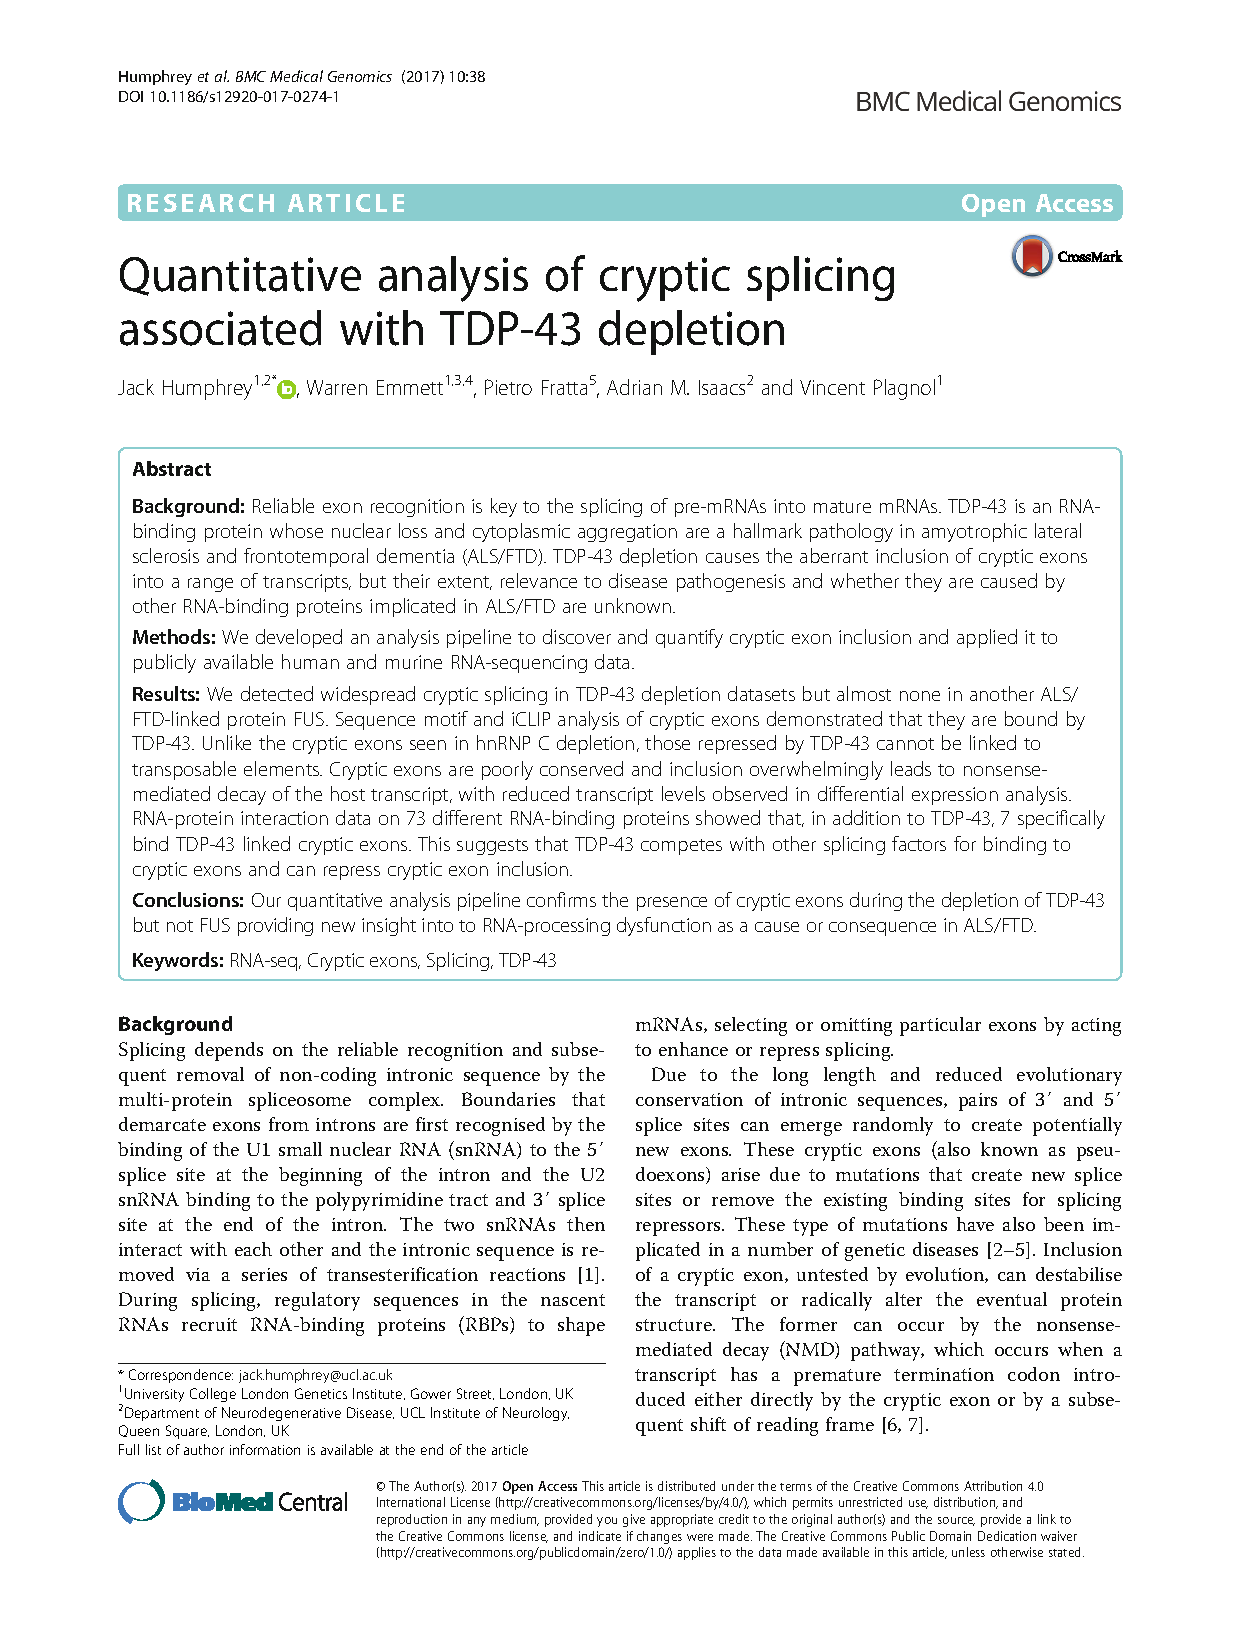
\includepdf[pages=-]{Appendices/Humphrey_Cryptic_Exons.pdf}

\includepdf[pages=-]{Appendices/Devoy_FUS_mouse.pdf}



%\subsection*{Annotation-free quanitification of RNA splicing with Leafcutter}
%
%While on a short fellowship at Stanford University, USA, I was involved in the development of Leafcutter, a software package to run differential splicing analysis on RNA-seq data. I designed and created an interactive web-based application for users to visualise and explore the results of using the tool. A screenshot from the tool is used in Figure 1 of the paper. I am an active maintainer of the Leafcutter Github repository (github.com/davidaknowles/leafcutter)
%\includepdf[pages=1-9]{Appendices/Li_Leafcutter.pdf}



% PUBLICATIONS - leave out for github
\input{Chapters/publications.tex}

\cleardoublepage
\end{document}